\chapter{CUORE}

CUORE (Cryogenic Underground Observatory for Rare Events) is located in Gran Sasso, Italy, and utilizes a bolometric method to search for \zeronubb. The experiment will run with 988 crystals of TeO$_2$ held at roughly 10 mK.
The source of \zeronubb~are the $^{130}$Te nuclei inside of the crystals ($34.2\%$ natural abundance \cite{Fehr200483}).
Thus, in this setup, the crystals act as both sources and detectors of \zeronubb. When energy is deposited in the crystals, such as from the electrons emitted during \zeronubb, the temperature of the crystals rises.
The Q-value of the decay of interest, viz. $^{130}\textrm{Te} \rightarrow ^{130}\textrm{Xe} + e + e$, is $2527.518\pm 0.013$ keV \cite{Redshaw:2009cf, Scielzo:2009nh, Rahaman:2011zz}.
This high Q-value is well-separated from other naturally occurring environmental $\gamma$'s except for $^{60}$Co at 2506 keV and $^{208}$Tl at 2615 keV.
However, the resolution of the CUORE crystals is $7.7\pm0.5$ keV, which means that these peaks do not significantly worsen the background in the region of interest at the Q-value.
In addition, this resolution aids in understanding background sources that deposit energy the detector as each \gamma~line can be observed above the Compton background, which aids in identifying particular background sources.

\section{CUORE Detectors}

\subsection{Particle Detection with Bolometers}
\label{ssec:Particle Detectrion with Bolometers}
As noted in \autoref{sec:State of Neutrinoless Double Beta Decay Experiments}, current experiments in the field of \zeronubb~use a wide array of technologies to identify \zeronubb~events.
However, CUORE utilizes a different method of calorimetry than its counterparts in that it uses a technique known as the bolometric method, which was first proposed for use in \zeronubb~experiments by Ettore Fiorini and Tapio Niinikosky \cite{FIORINI198483}.
As particles pass through matter, the energy they deposit is eventually carried into the surrounding material as heat.
This method requires a mass that acts as a thermal capacitor, a weak thermal connection to a heat bath, and a thermometer (generally a thermistor) and CUORE's setup is sketched in \autoref{fig:thermal_crystal_cartoon} and a sample pulse is shown in \autoref{fig:Sample_pulse}.
The detectors in CUORE, $\textrm{TeO}_2$~crystals, respond to energy deposition by a temperature rise according to
\begin{equation}
\delta T = \delta E/C(T).
\end{equation}
At low C, $\delta T$ is maximized; therefore, the crystals are operated at low temperatures where C(T) is given by the Debye Model:
\begin{equation}
C(T)\sim (\frac{T}{\Theta_D})^3
\end{equation} 
where $\Theta_D$ is the Debye temperature for \teotwo, $232\pm7~\textrm{K}$ \cite{BolometerCalculations}. This strong temperature dependence on the heat capacity is what drives the need for low temperatures in CUORE, where we have achieved an operational temperature of $\sim10$ mK.
The custom cryostat used to do this is described later on in \autoref{sec:CUORE Cryostat}.
At these temperatures, a 1 MeV energy deposit in a single CUORE crystal would cause the temperature to rise to $\sim 100~\textrm{\mu K}$. 

\begin{figure}[htbp]
\centering
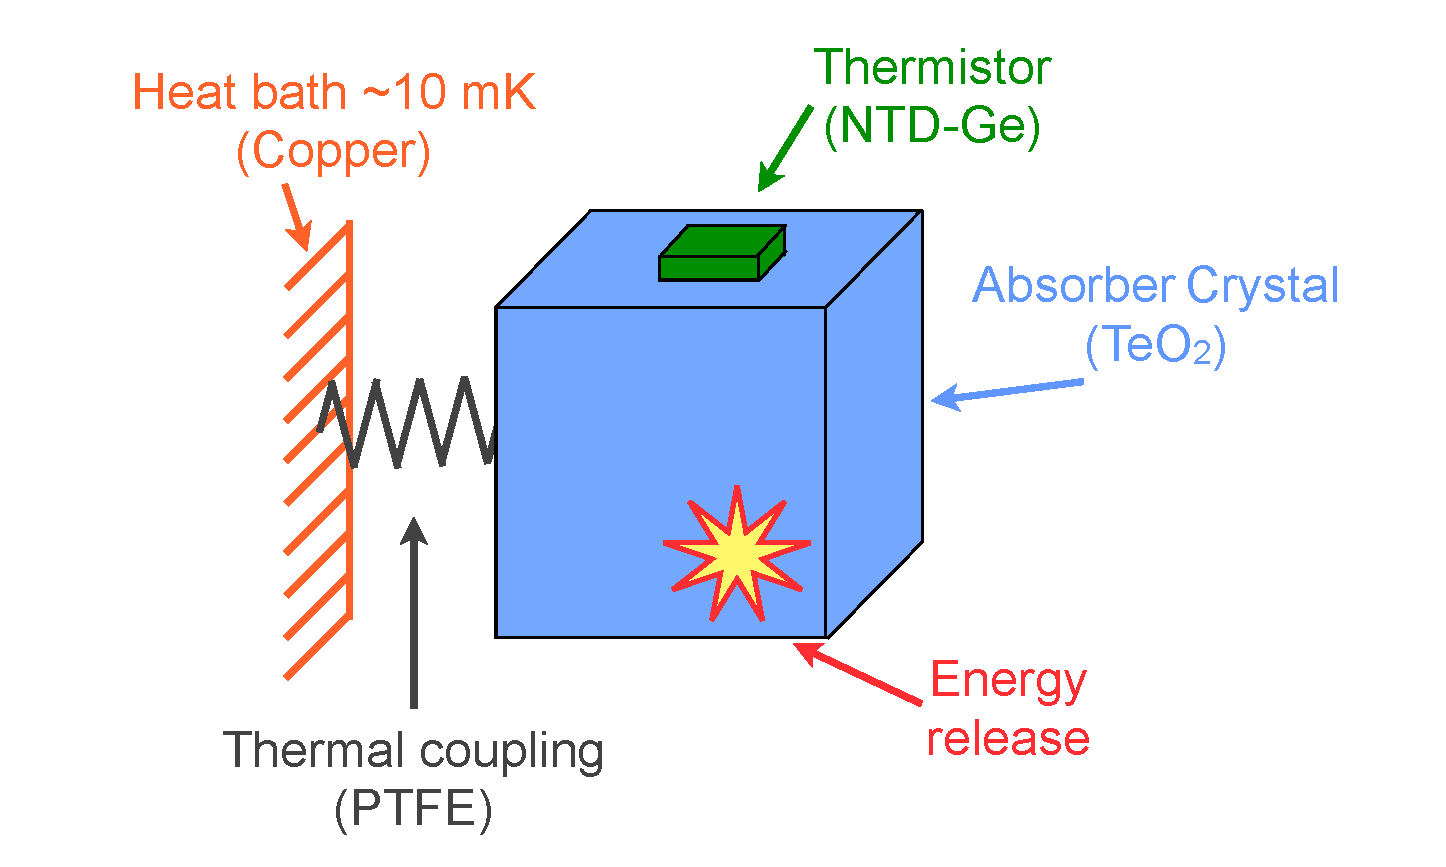
\includegraphics[width=0.7\linewidth]{Figures/bolosketch-color.pdf}
\caption[A diagram of the thermal connection of the TeO$_2$ crystals to the thermal bath provided by the copper frames.]
{A diagram (not to scale) of the thermal connection of the TeO$_2$ crystals to the thermal bath provided by the copper frames.
The weak thermal coupling is provided by the PTFE.}
\label{fig:thermal_crystal_cartoon}
\end{figure}

\subsubsection*{Bolometer Thermometry Instrumentation}
Of course, an integral component to the bolometric method is the choice of thermometer used to detect these changes in temperature.
The choice of thermometer that CUORE uses is a Neutron Transmutation Doped (NTD) germanium thermistor due to its reproducibility and uniformity, which is critically important across CUORE's crystal array. However, a drawback to this is that each NTD thermistor must be individually cut from a block and then mounted onto each bolometer \cite{NTDThermistor}.

\begin{figure}[htbp]
%\captionsetup[subfigure]{justification=centering}
\centering
\begin{subfigure}[t]{0.40\textwidth}
\centering
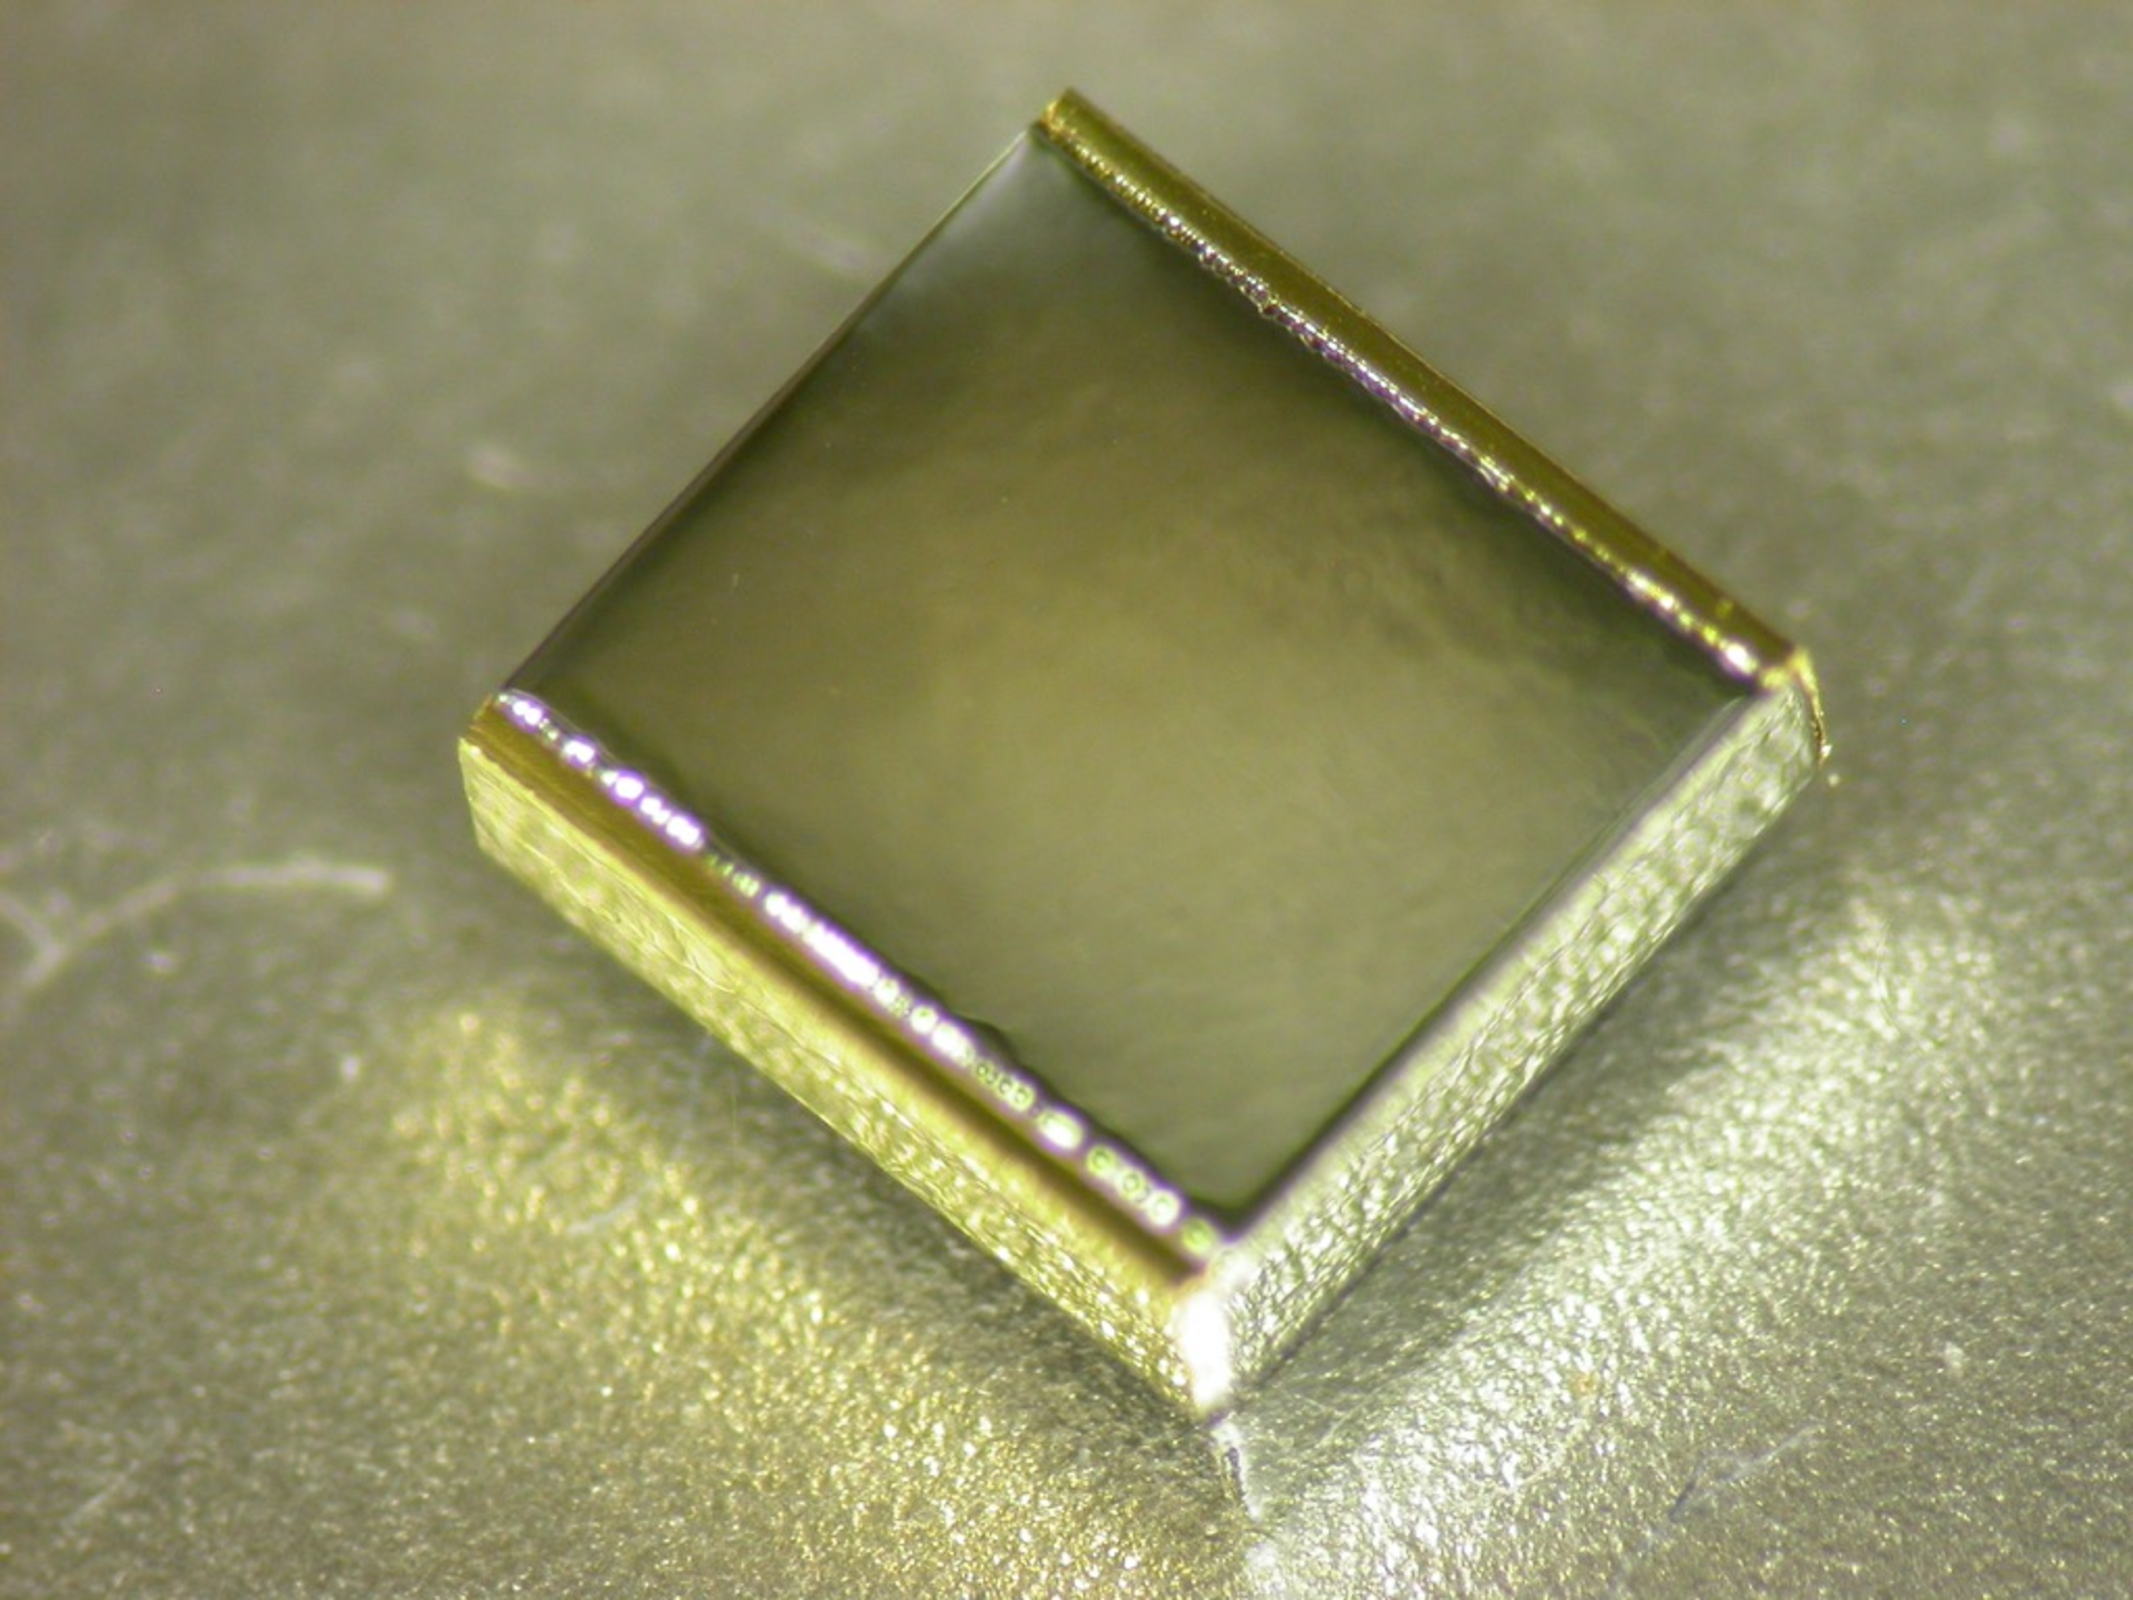
\includegraphics[width=0.9\textwidth]{Figures/fig04a.pdf}
\caption{}
\label{fig:NTD_picture}
\end{subfigure}
\qquad
\begin{subfigure}[t]{0.40\textwidth}
\centering
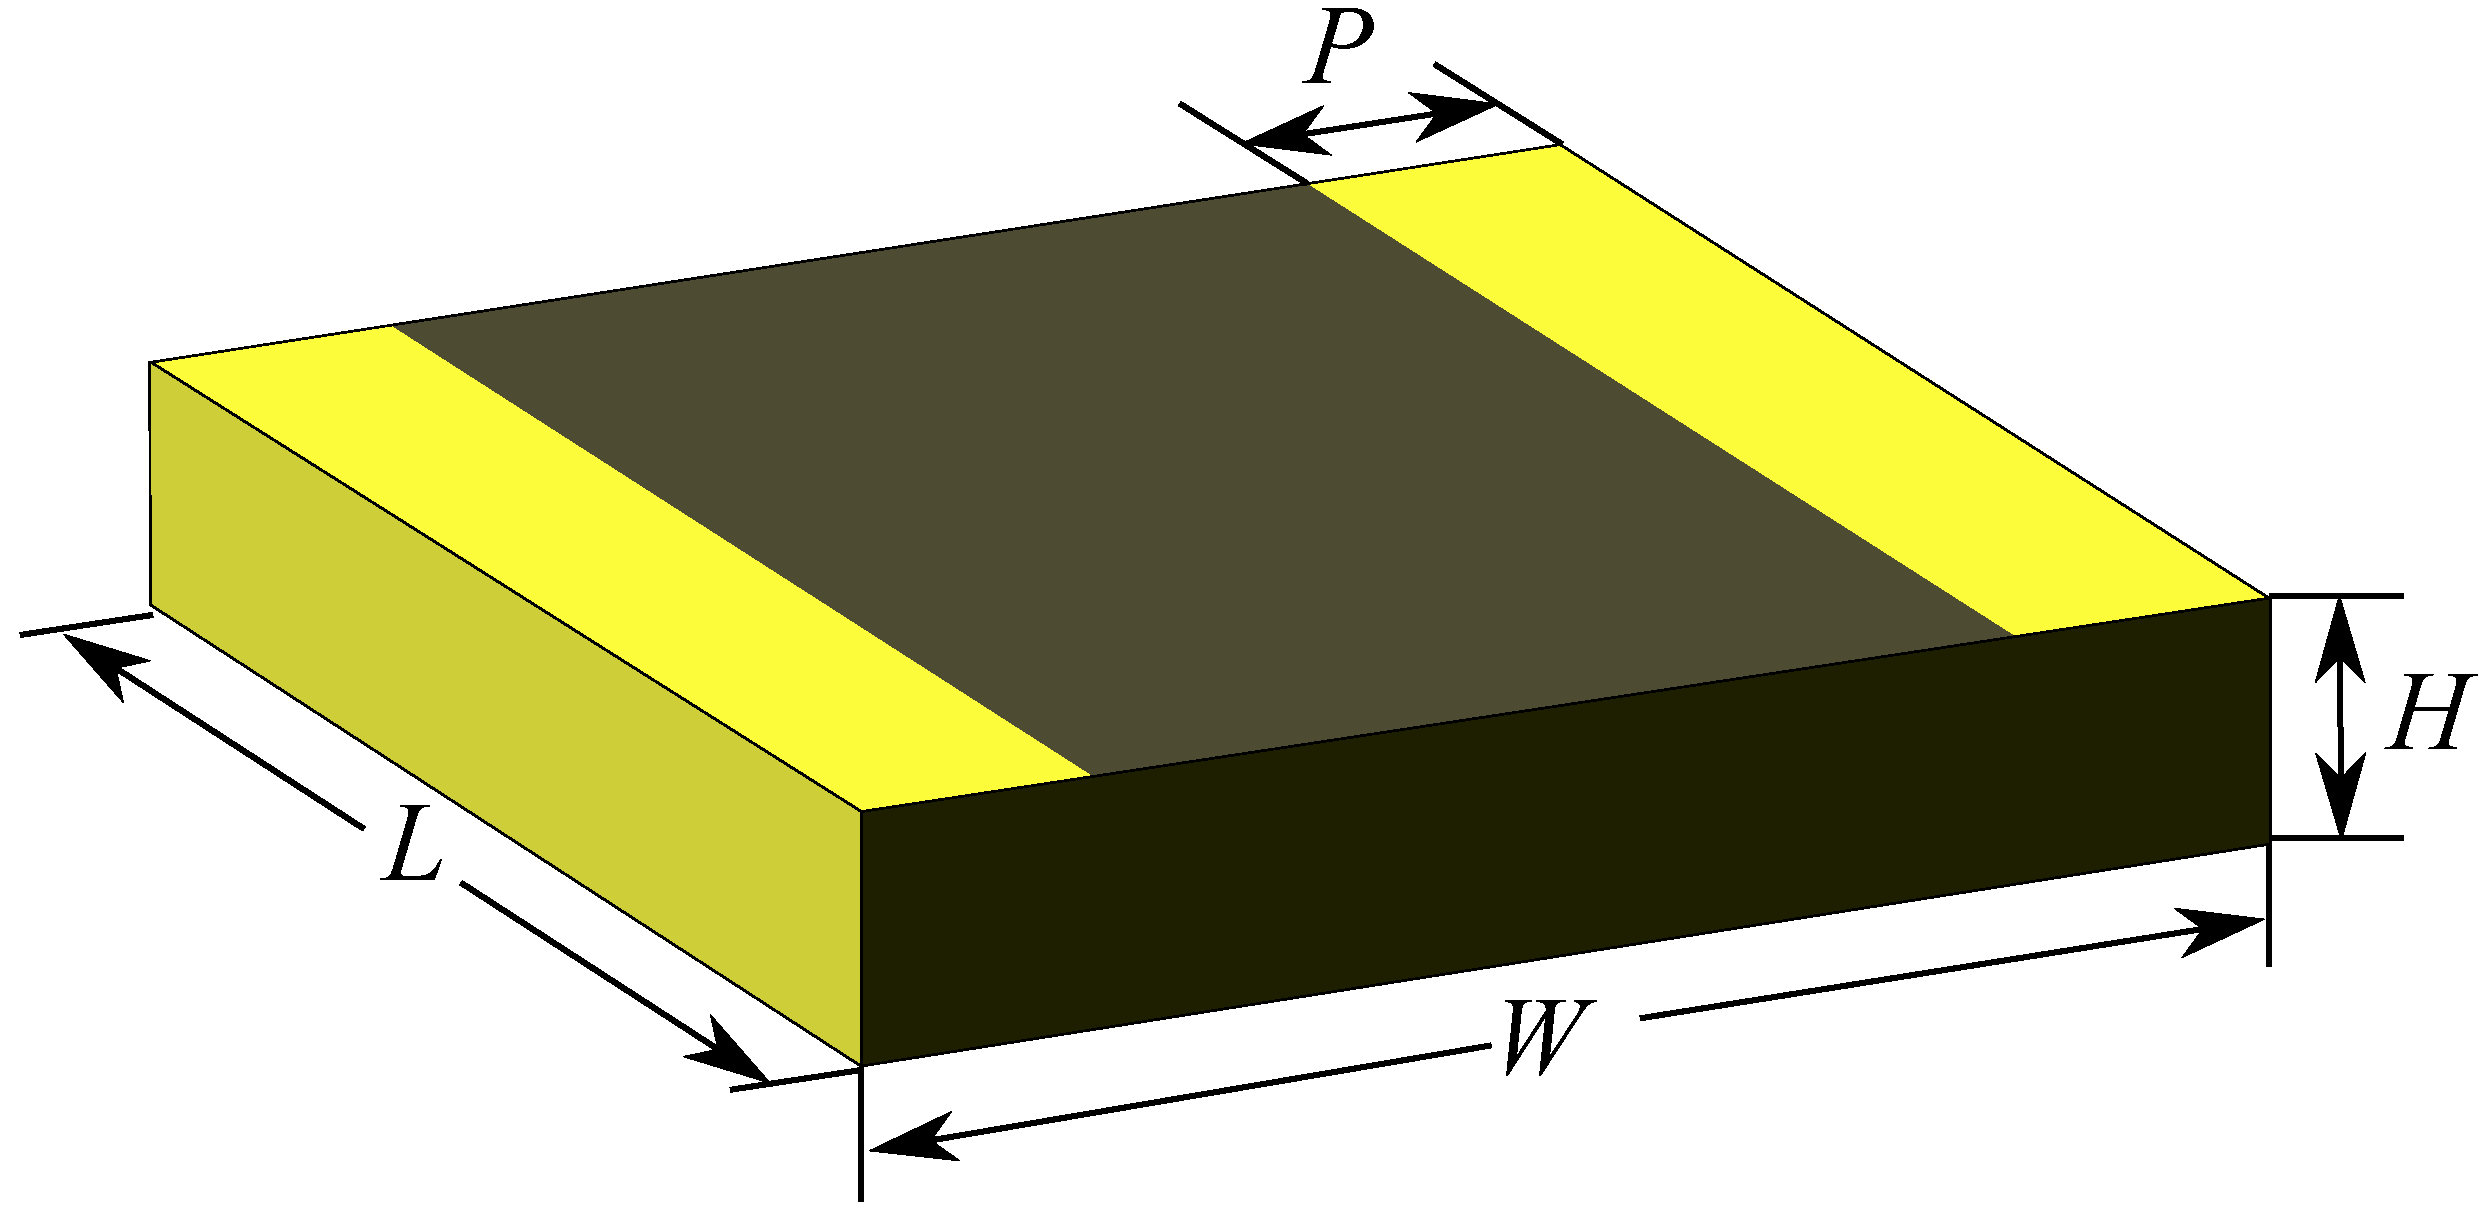
\includegraphics[width=0.9\textwidth]{Figures/fig04b.pdf}
\caption{}
\label{fig:NTD_sketch}
\end{subfigure}
\caption[A photograph (a) and a diagram (b) of an NTD thermistor used in CUORE.]
{A photograph (a) and a diagram (b) of an NTD thermistor used in CUORE.
The dimensions of the NTD are $3.0\times2.9\times0.9~\textrm{mm}^3$ ($\textrm{L} \times \textrm{W} \times \textrm{H}$ with $\textrm{P}=0.2~\textrm{mm}$.
Figure from \cite{Alduino:2016vjd}.}
\label{fig:NTD}
\end{figure}

The NTD thermistors are created by irradiating pure Ge with a flux of thermal neutrons, and the NTD sensors used in CUORE were irradiated at the MIT Nuclear Reactor Laboratory.
This flux produces Ga, As, and Se, which dopes the Ge, and the doping stops before the Ge reaches a critical doping threshold such that it still remains a semiconductor.
Above this threshold, the Ge material acts as a metal where resistivity goes to 0 at 0 K, but just below this threshold, the resistivity increases sharply.
This is due to the fact that the doping causes conduction electrons in the material to localize into the doped atoms which are spread out into the germanium.
When conducting at high temperatures, the electrons tunnel to the nearest available unoccupied sites in the material.
At low temperatures, however, such as the $<1~\textrm{K}$ temperatures of the CUORE detectors, the resulting lack of higher-energy phonons prevents the electron from tunneling into the nearest sites, and instead favor sites with similar energies to the electron.
In this regime of ``variable range hopping", the resistance of the NTD goes as
\begin{equation}
    R(T) = R_0 e^{\left(\frac{T_0}{T}\right)^p} 
    \label{eq:NTD_Resistivity}
\end{equation}
as shown by Shklovskii and Efros \cite{NTDResistivity}.
This causes the resistivity to have a strong temperature dependence at cryogenic temperature and allows the NTD thermistor to serve as a highly sensitive thermometer to measure the temperature rise as a voltage, as shown in \autoref{fig:Sample_pulse}.
For the NTDs used on the CUORE-0 detectors, the measured values for $T_0$ and $R_0$ are 3.84 K and 1.13 $\Omega$, respectively, corresponding to a resistance of 0.37 G$\Omega$ at 10 mK \cite{Alduino:2016vjd}.
The NTDs used on the CUORE towers have slightly higher resistances, with an average resistance of 0.6-1.1 G$\Omega$ \cite{Nutini:LoadCurves}.

\begin{figure}[htbp]
\centering
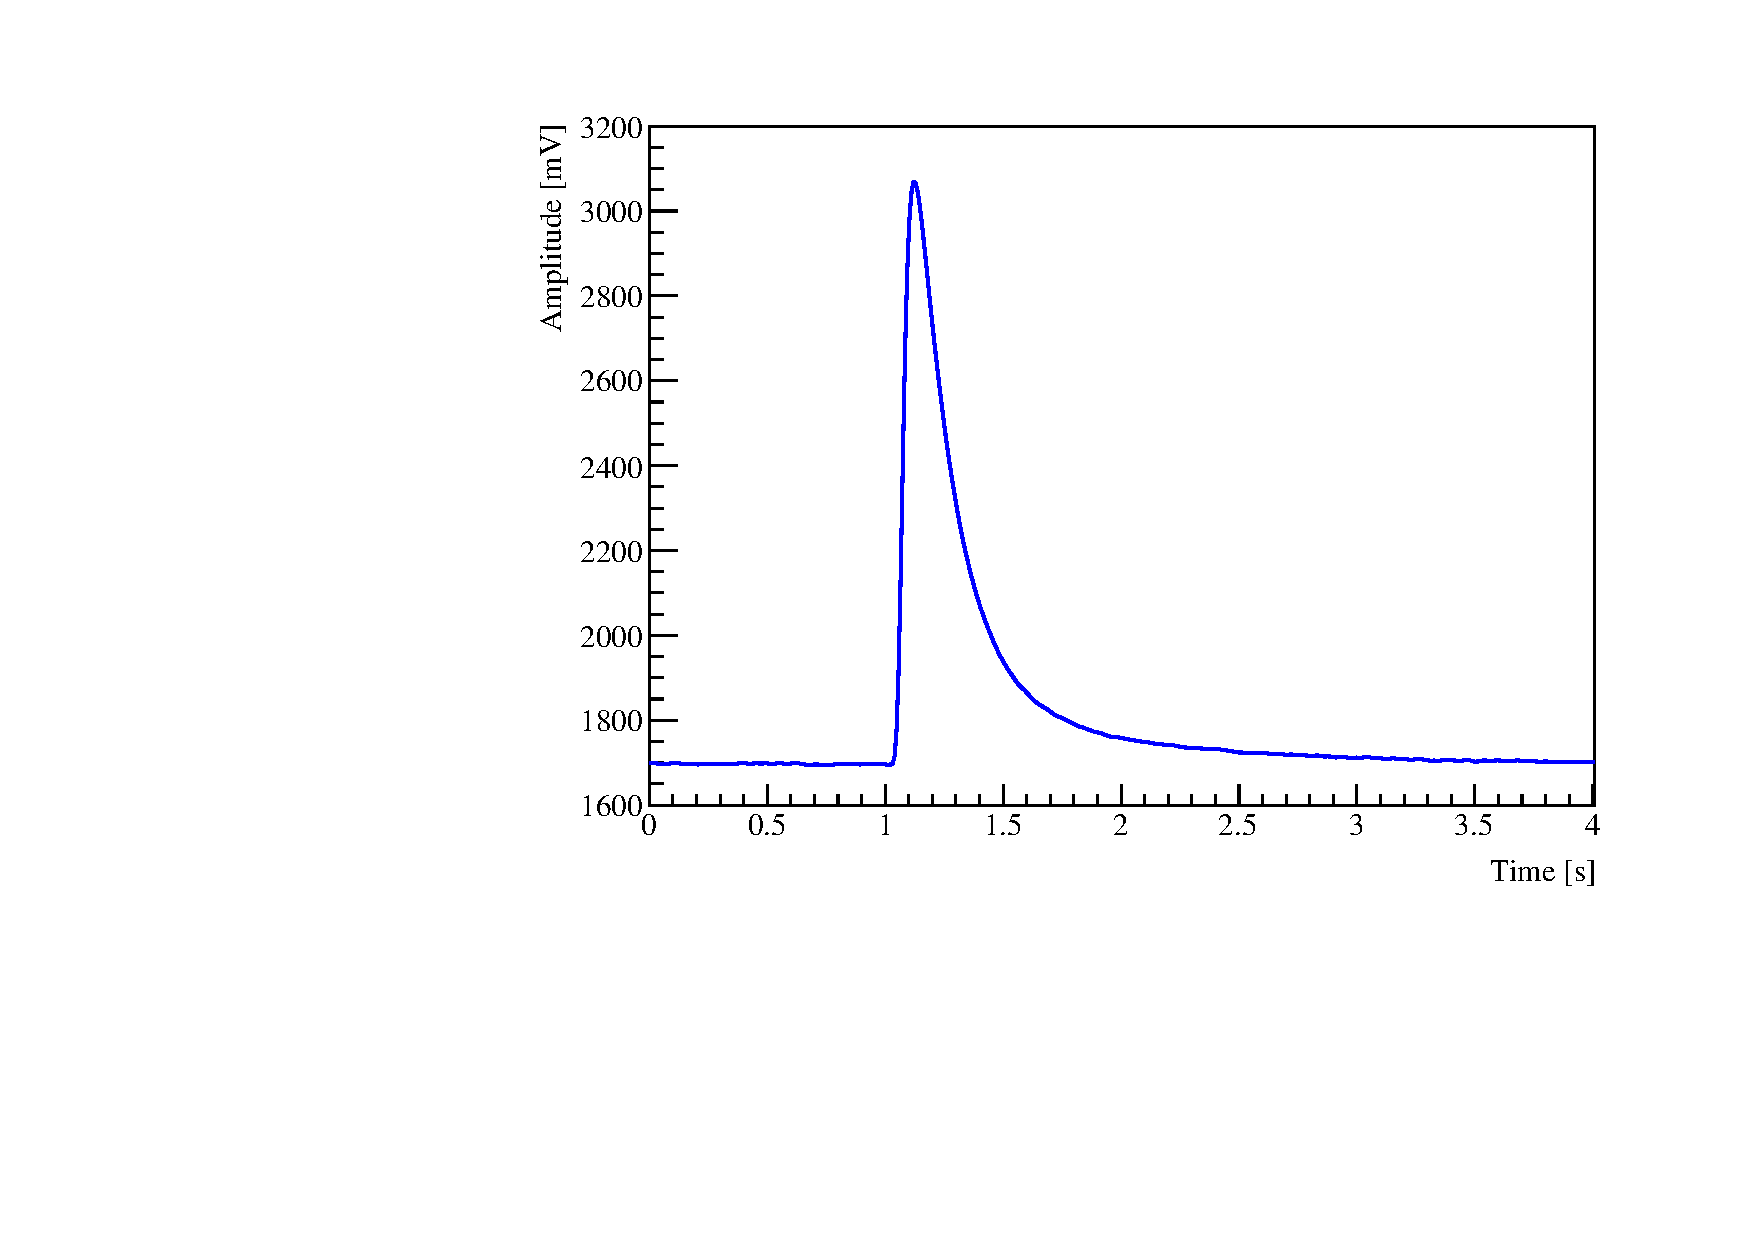
\includegraphics[width=0.7\linewidth]{Figures/pulse-conference.pdf}
\caption[An example pulse from a single CUORE detector measured by an NTD Ge thermistor.]
{An example pulse from a single CUORE detector measured by an NTD Ge thermistor.
After an event at 1 s where energy is deposited in the crystal, a fast (0.1 s) temperature rise is observed followed with a slow (3 s) cooling through the weak coupling to the thermal bath.}
\label{fig:Sample_pulse}
\end{figure}

\subsubsection*{Silicon Heater}
While the detectors are calibrated through physics events on a $\sim$ monthly basis by the calibration system, discussed more in \autoref{chap:DCS}, additional and continuous stabilization is provided through direct heating of the bolometers through a silicon heater that is also attached onto the bolometer, discussed more in \autoref{ssec:Stabilization}.
These heaters are custom-designed $2.33\times2.40\times0.52~\textrm{mm}^3$ high-purity Si chips, shown in \autoref{fig:Si_heater}.
They were manufactured by Istituto per la Ricerca Scientifica e Tecnologica (IRST, now Fondazione Bruno Kessler) in Trento, Italy.
As current passes through these Si chips with resistance $\approx300~\textrm{k}\Omega$, power is dissipated through ohmic losses in the heaters into the bolometers, which is then measured by the NTDs.
By pulsing these heaters with a known energy, the detector response can then be stabilized at various detector baselines.

\begin{figure}
    \centering
    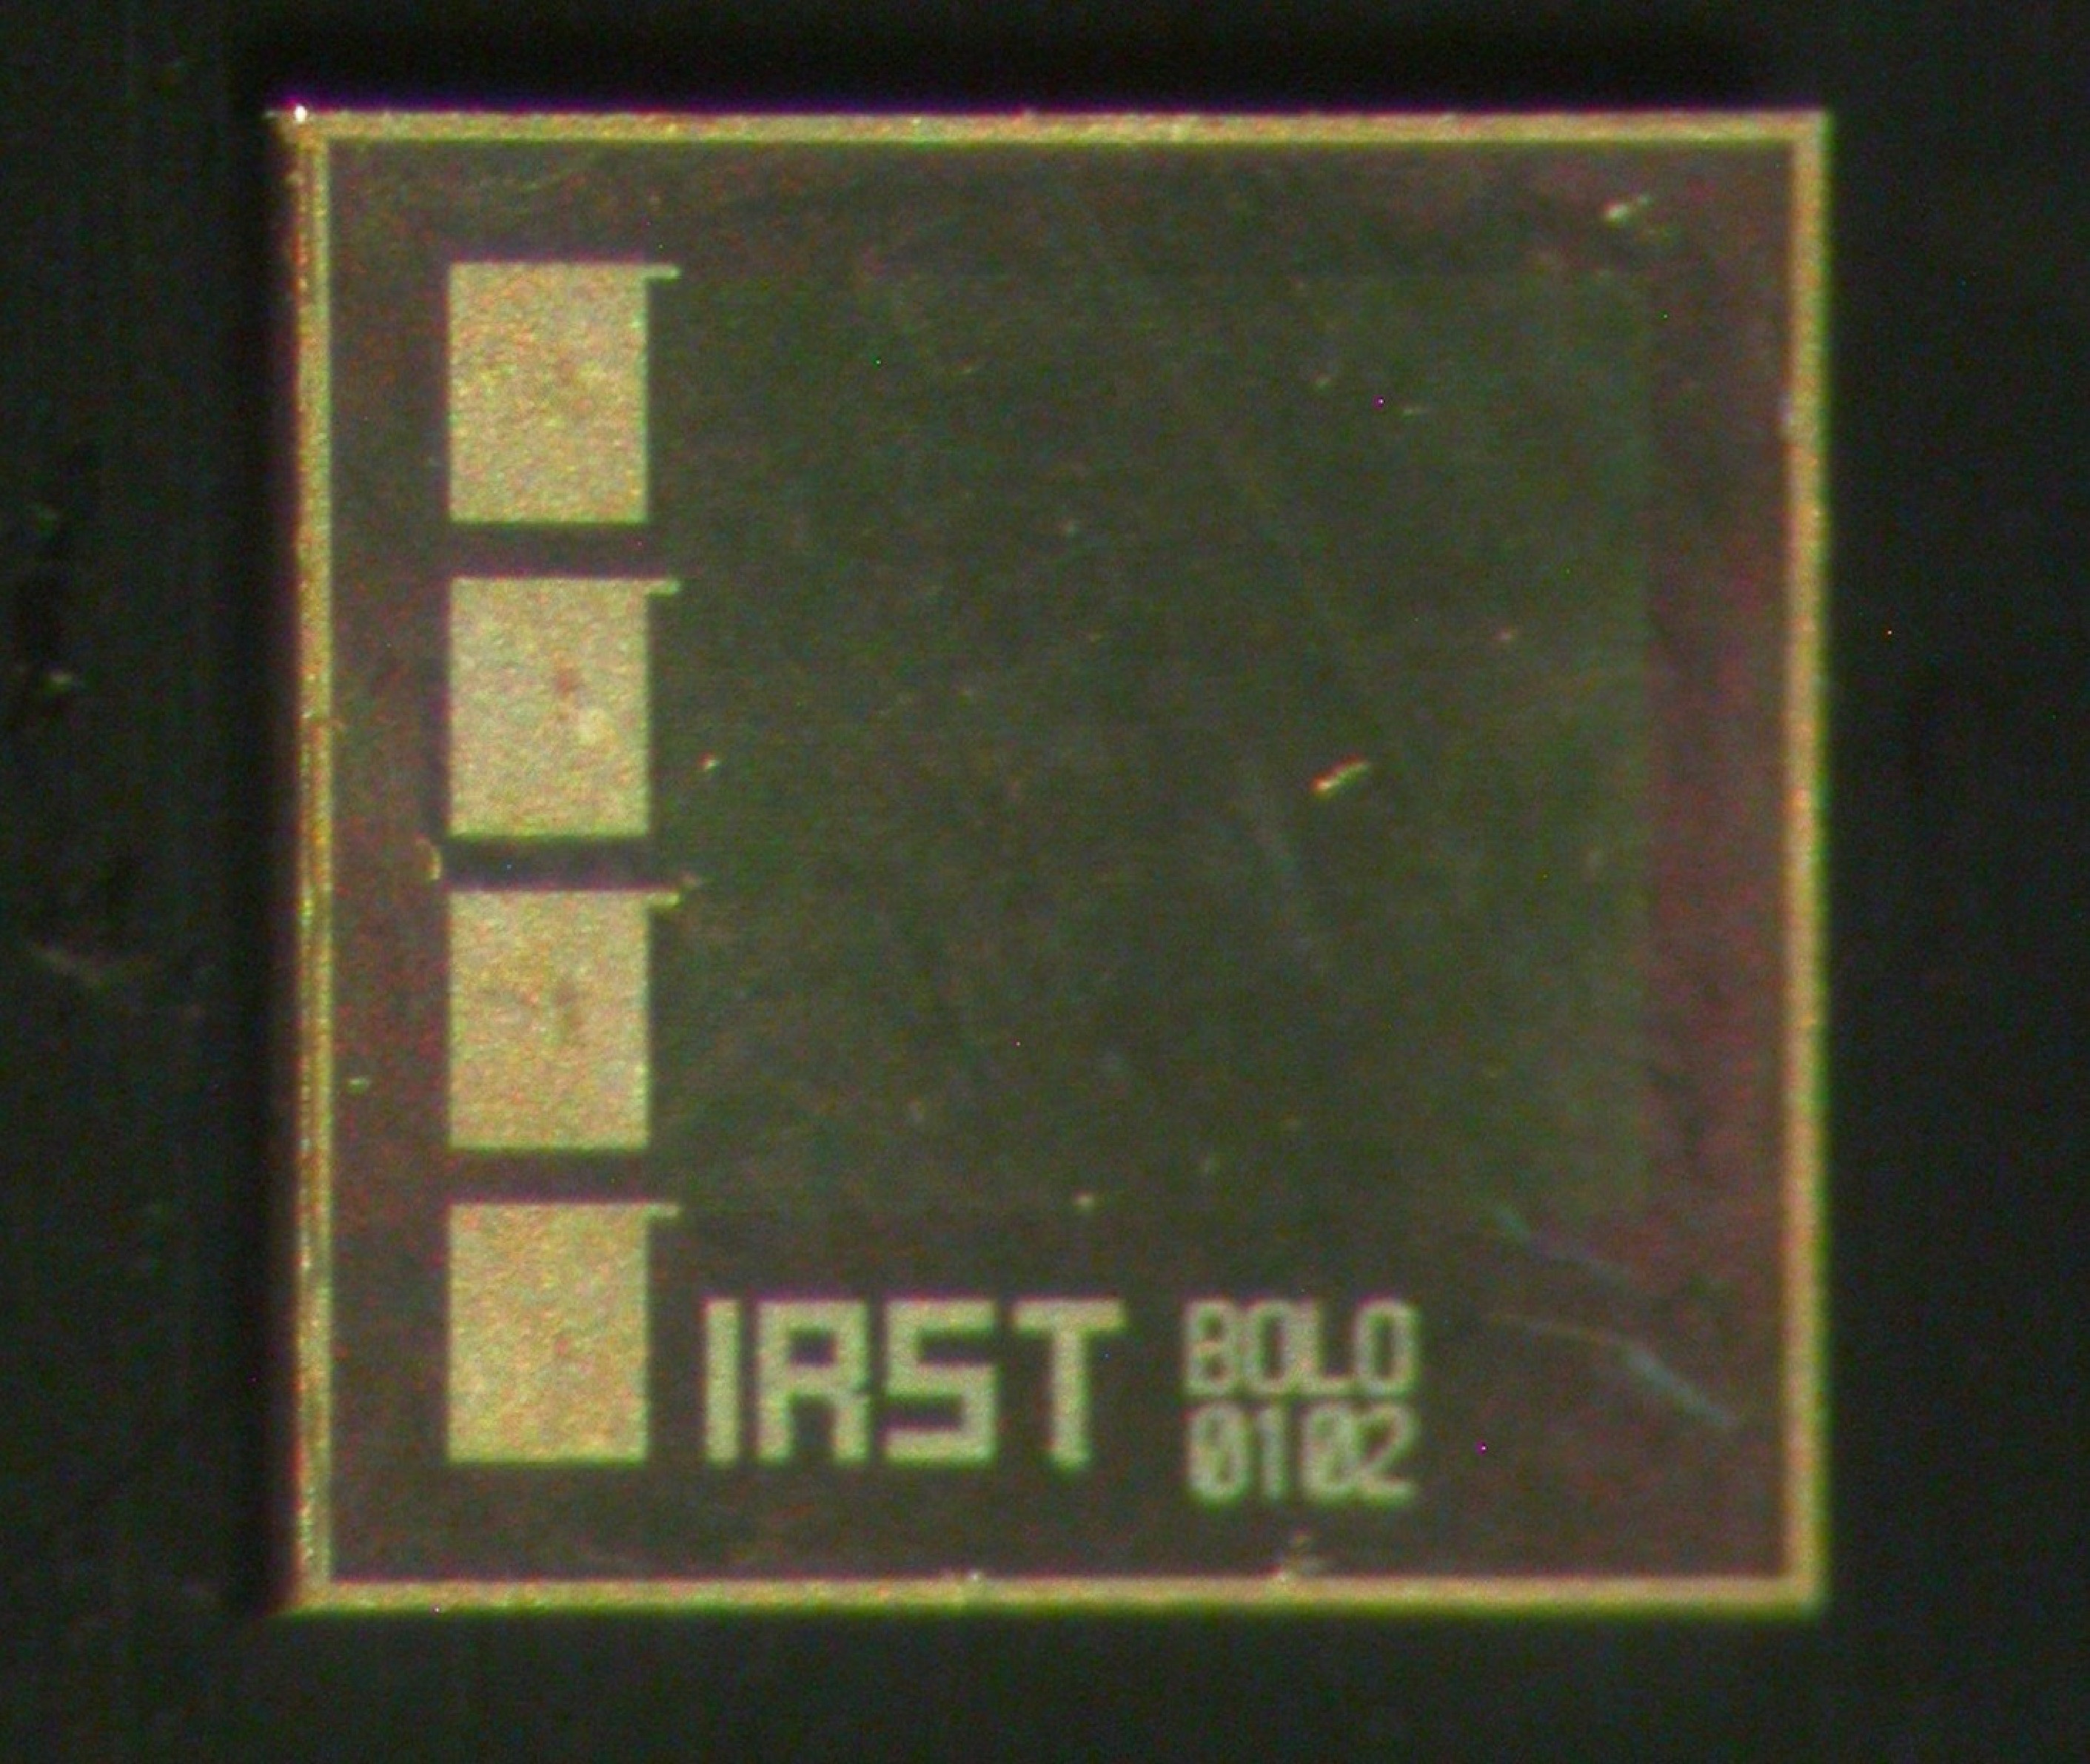
\includegraphics[width=0.4\linewidth]{Figures/fig05a.pdf}
    \caption[Photograph of a silicon heater.]
    {Photograph of a silicon heater.
    There are four aluminum pads on the chip, and, depending on the pair of pads connected, the resistance across the heater can be 100, 200, or 300 k$\Omega$.}
    \label{fig:Si_heater}
\end{figure}

\subsubsection*{Cables and Glue}
The heaters and thermistors need to be attached to the crystals with a strong thermal and mechanical coupling to work properly.
This is done by Araldite Rapid\footnote{\RaggedRight\url{http://www.go-araldite.com/products/epoxy-adhesives/araldite-rapid-2-x-15ml-tube}}
epoxy which is deposited in a pattern of glue spots shown in \autoref{fig:glue}.

\begin{figure}[htbp]
%\captionsetup[subfigure]{justification=centering}
\centering
\begin{subfigure}[t]{0.45\textwidth}
\centering
    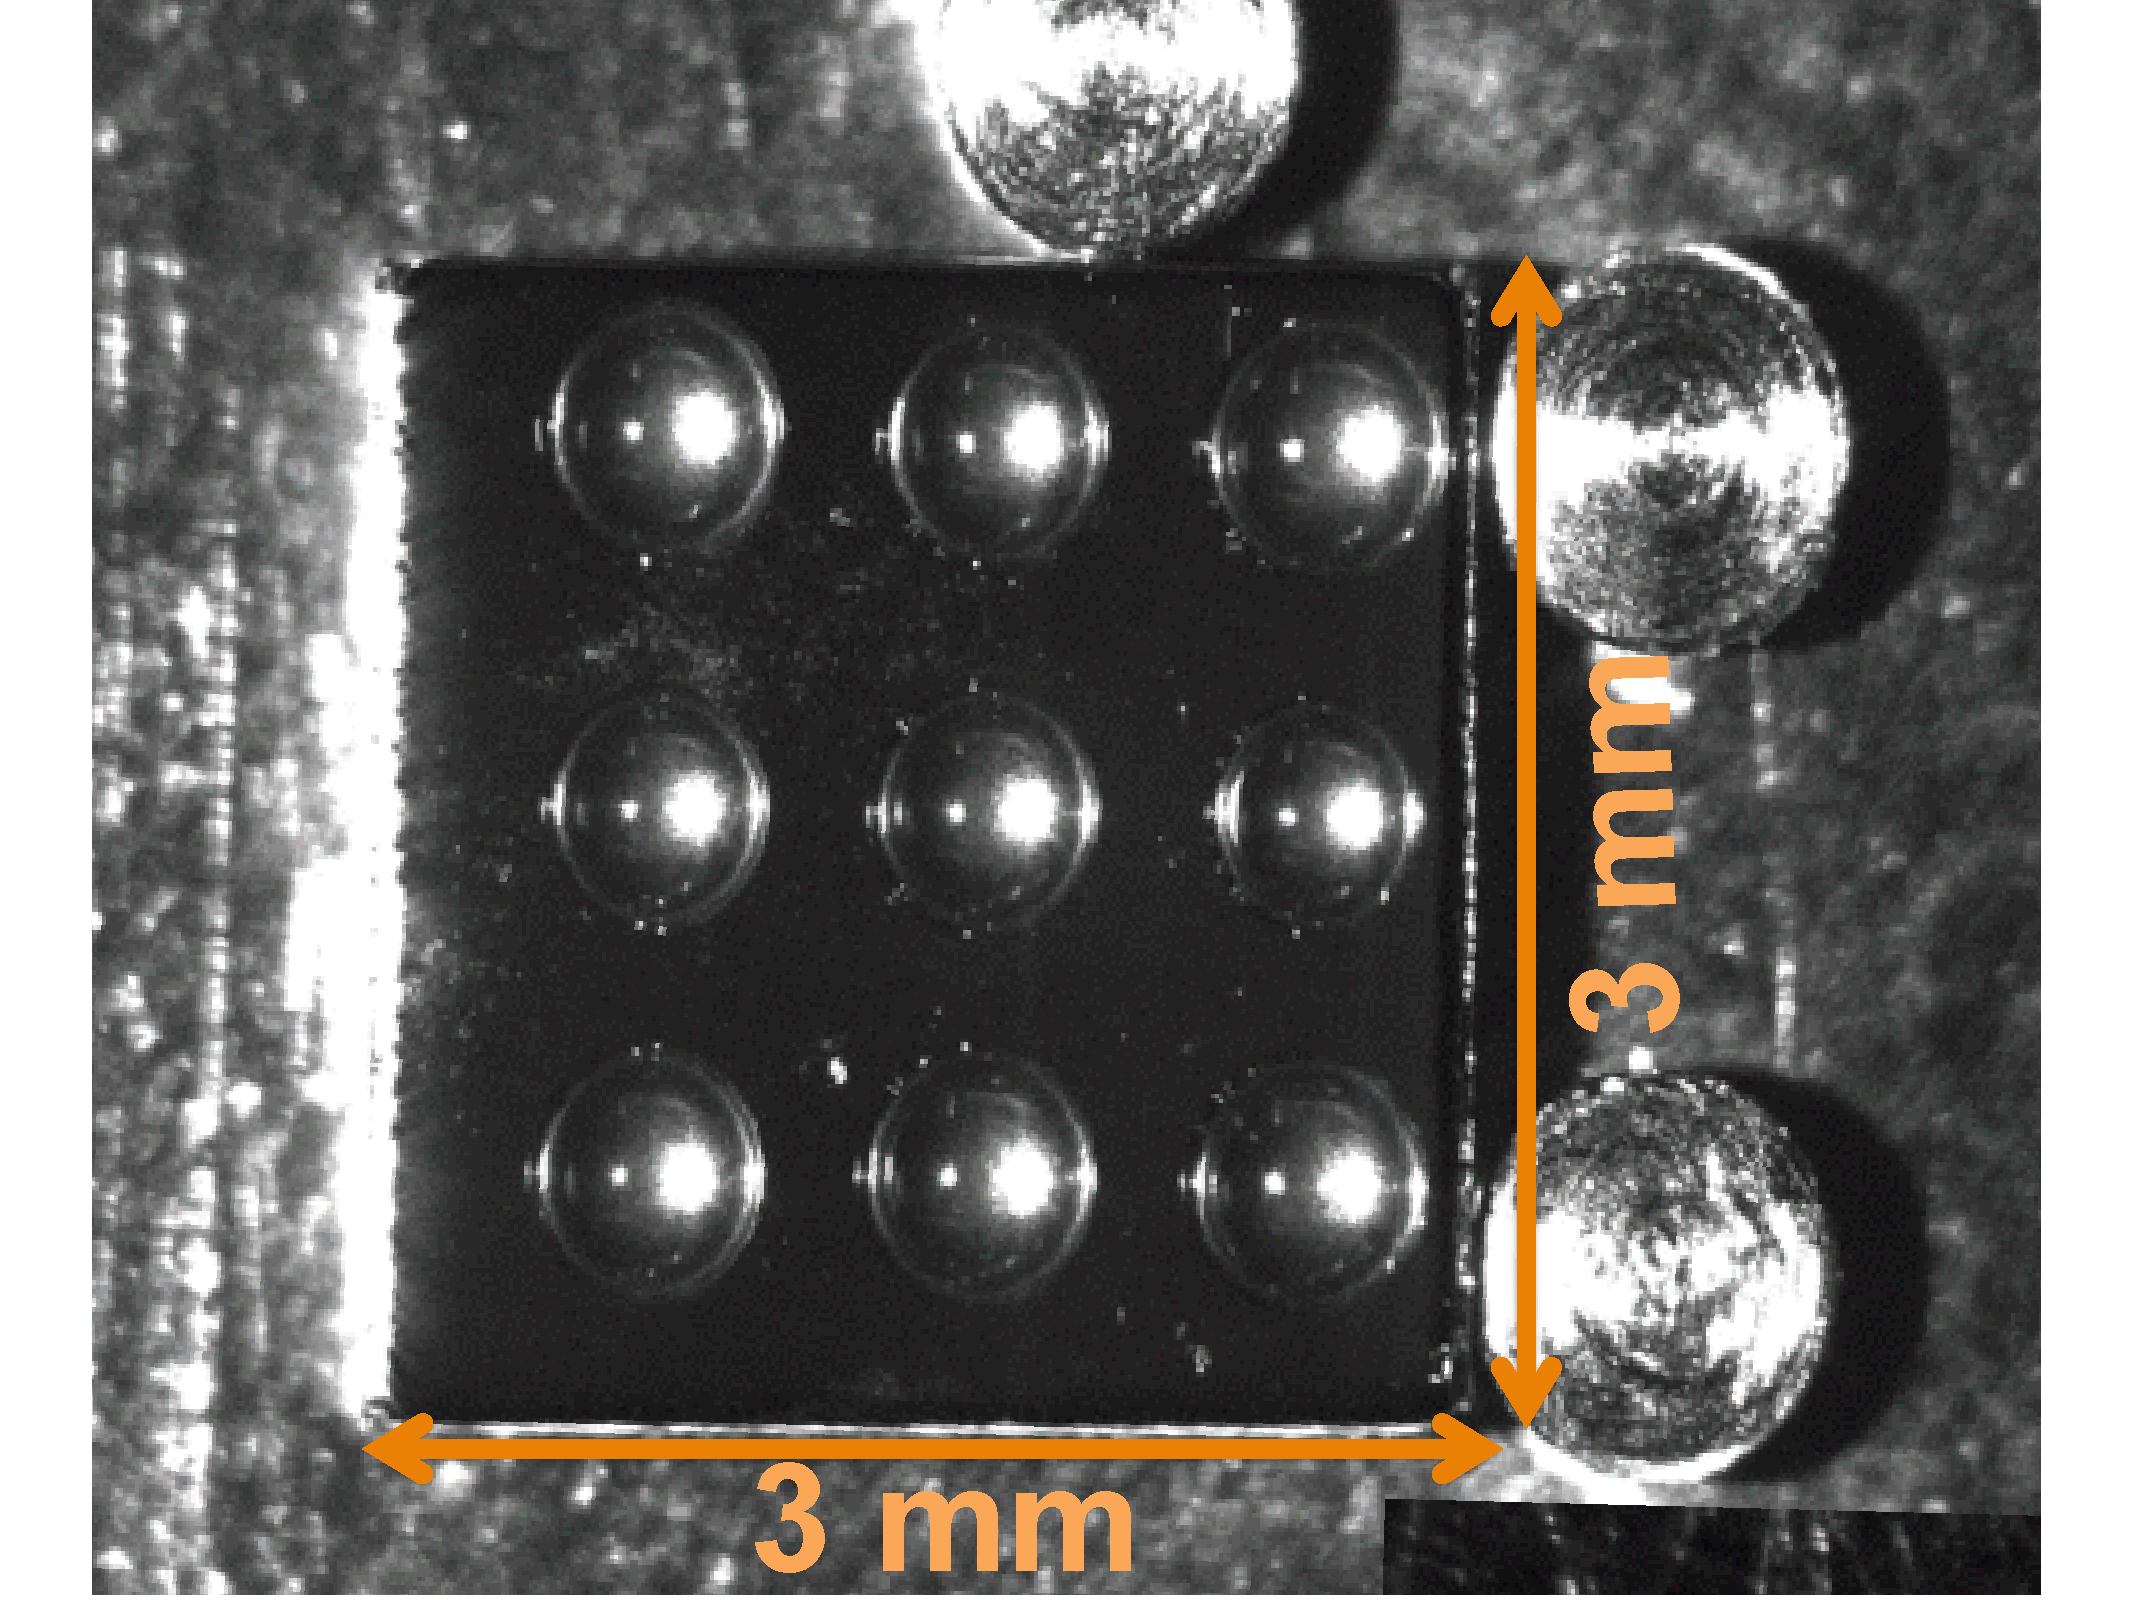
\includegraphics[width=0.95\linewidth]{Figures/fig10a.pdf}
\caption{}
\label{fig:glue_NTD}
\end{subfigure}
\qquad
\begin{subfigure}[t]{0.45\textwidth}
\centering
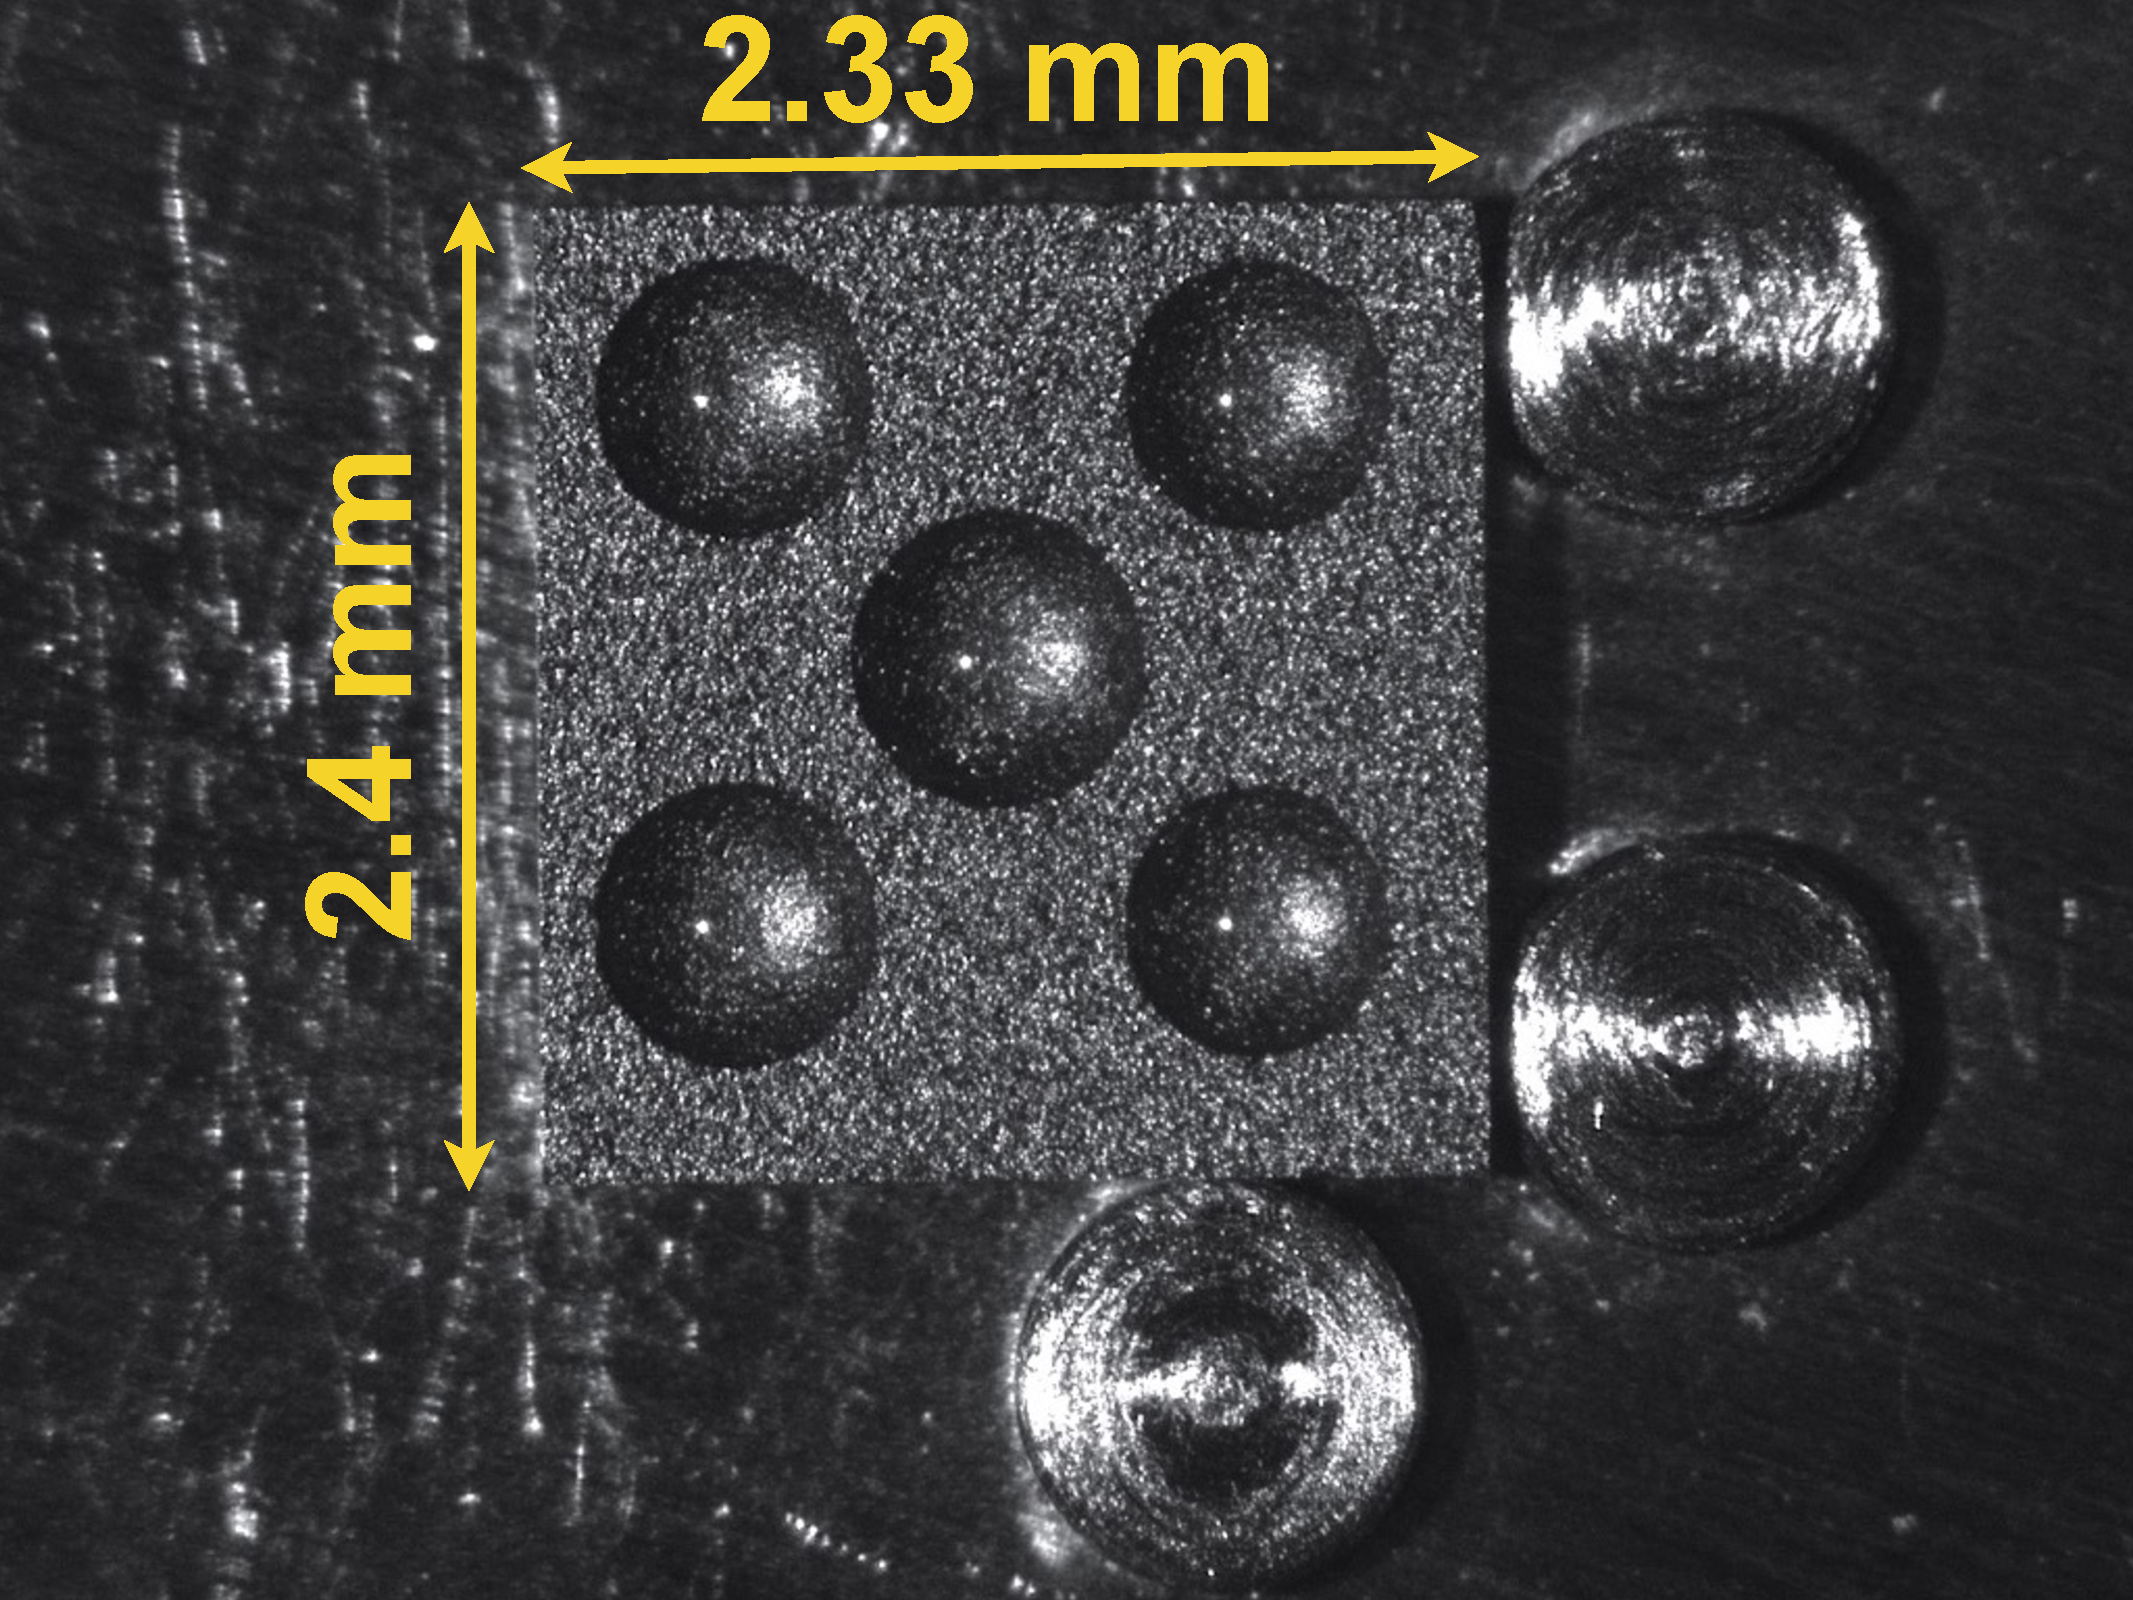
\includegraphics[width=0.95\textwidth]{Figures/fig10b.pdf}
\caption{}
\label{fig:glue_Si}
\end{subfigure}
\caption[Photographs of the glue spots on the CUORE NTD (a) and Si heater (b).]
{Photographs of the glue spots on the CUORE NTD (a) and Si heater (b).
The NTD has a pattern of 9 glue spots and the heater has a pattern of 5 glue spots, applied robotically.
Figure from \cite{Alduino:2016vjd}.}
\label{fig:glue}
\end{figure}

After being glued to each detector, the heater and NTD need to also be connected to the readout electronics.
To achieve this, gold cables are bonded to the pads of the copper tape that is connected to the readout electronics.
Since the NTDs are critically important to the operation of the experiment, these gold cables are doubled for redundancy in case of a poor connection.

\begin{figure}[htbp]
%\captionsetup[subfigure]{justification=centering}
\centering
\begin{subfigure}[t]{0.45\textwidth}
\centering
    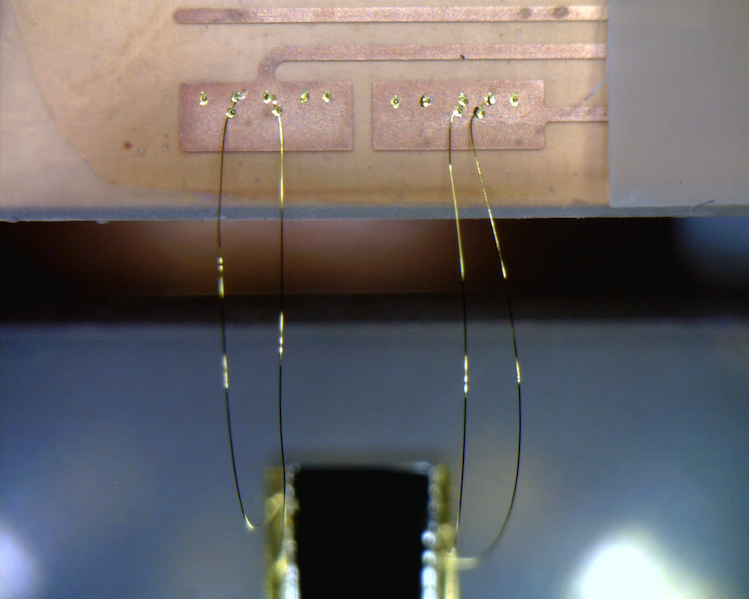
\includegraphics[width=0.95\linewidth]{Figures/NTD_bond.png}
\caption{}
\label{fig:bond_NTD}
\end{subfigure}
\qquad
\begin{subfigure}[t]{0.45\textwidth}
\centering
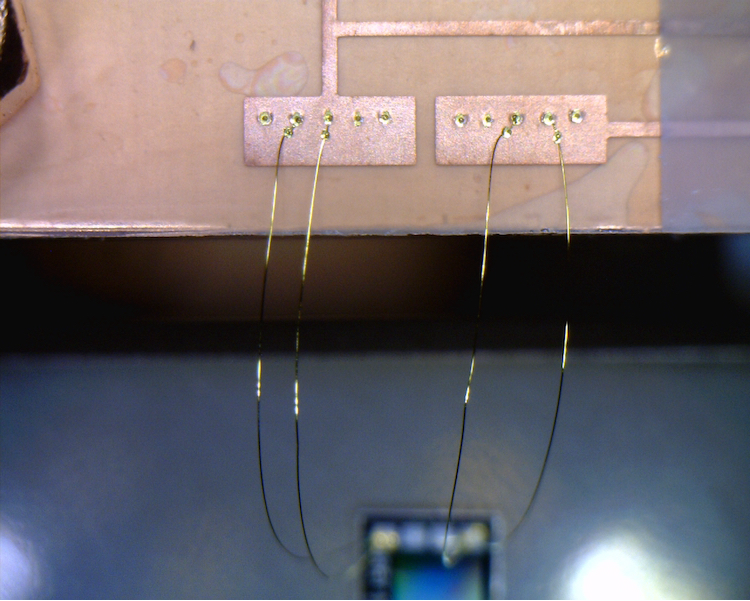
\includegraphics[width=0.95\textwidth]{Figures/Si_bond.png}
\caption{}
\label{fig:bond_Si}
\end{subfigure}
\caption[Photographs of the gold wire bonds on a CUORE NTD (a) and Si heater (b).]
{Photographs of the gold wire bonds on a CUORE NTD (a) and Si heater (b).
Figure courtesy of the CUORE collaboration.}
\label{fig:bonds}
\end{figure}

\subsubsection*{Bolometric Method Drawbacks}
There are some particular challenges to the bolometric method, however.
The dependence on the heat capacity of the crystal depends on the exact crystalline structure of the crystal, which requires regular calibrations due to possible minute changes.
In addition, this strong temperature dependence, while useful for identifying signal, needs a well-stabilized detector with few disturbances from non-particle thermal sources and a consistent and well-understood temperature baseline.
Finally, the long time constant of the cooling of the crystal, which is generally a few seconds for a 1 MeV pulse, requires that there be a low rate of events in the crystal.
This requirement of a low rate is generally not an issue for physics datataking, as the background rates are necessarily low due to the sensitivity requirements of a \zeronubb~search, but this limits the time it takes to calibrate the bolometer\footnote{This generally becomes an optimization problem, later discussed in \autoref{chap:DCS}, where the time it takes to calibrate a detector with 100 events can be reduced by reducing the activity of a calibration source.}.


\subsection{CUORE Detector Array}
CUORE uses 988 \teotwo~crystals as bolometers arranged in 19 towers with 13 floors as shown in \autoref{fig:cuore_detector_array} and \autoref{fig:cuore_photograph}.
These crystals are $5\times5\times5~\textrm{cm}^3$ in size and have mass 750 g each, for a total of 742 kg of \teotwo.
The crystals are grown by The Shanghai Institute of Ceramics, Chinese Academy of Sciences (SICCAS) \cite{Arnaboldi:2010fj} and shipped to Italy by boat, avoiding air travel in order to minimize cosmogenic activation \cite{Barghouty:2010kj}.
Taking advantage of the relatively high natural isotopic abundance of Te, shown in \autoref{fig:q_vs_ia-color}, this comes to a total mass of 206 kg of $^{130}$Te and 189 kg of $^{128}$Te.
Each tower is approximately 80 cm tall, such that in operation, these crystals form the coldest cubic meter in the known universe \cite{Ouellet:2014qua}.

\begin{figure}
    \centering
    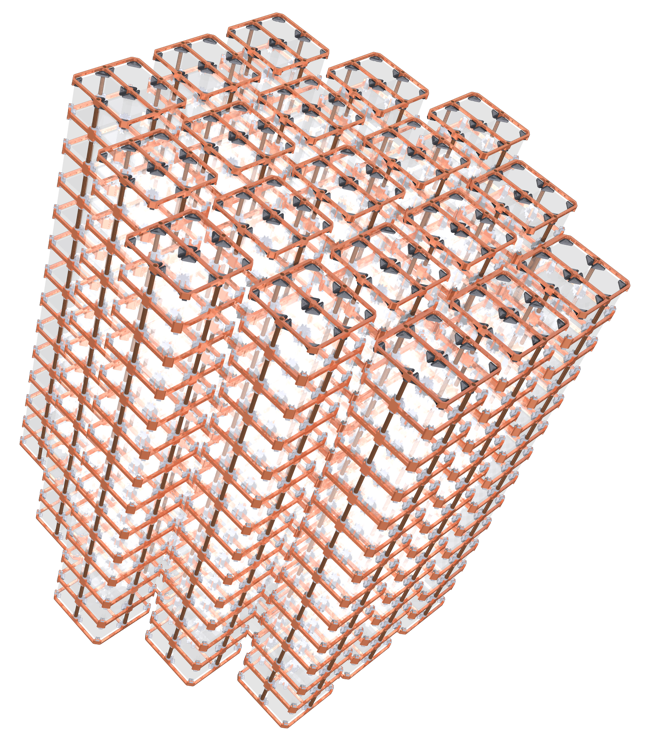
\includegraphics[height=4in]{Figures/CUORE_detector_array_0.png}
    \caption[A schematic of the CUORE detector array.]
    {A schematic of the CUORE detector array.
    The detectors are held in place by the copper frames and arranged in 19 towers with 13 floors each.
    The position of the detector array relative to the rest of the cryostat can be seen in \autoref{fig:cryostat_cad_cutout}.}
    \label{fig:cuore_detector_array}
\end{figure}

Another benefit to using a bolometric method for particle detection is that it enables a ``source $=$ detector" style experiment such that the \zeronubb~and \twonubb~decays happen directly inside the detectors themselves.
This both reduces the amount of material and associated radioactive backgrounds needed in the experiment and also increases the signal detection efficiency of \zeronubb~and \twonubb-like decays.

In order to arrange these bolometers into these 19 towers, the \teotwo~crystals are held together inside copper frames with polytetrafluoroethylene (PTFE) holders.
These holders are designed such that the crystals are held in place firmly at the low temperatures in CUORE\footnote{Although, one of the benefits of using \teotwo~is that its thermal contraction is similar to that of copper, with values of $\Delta l/l \approx 0.27\%$ and $\Delta l / l \approx 0.33\%$, respectively \cite{ALESSANDRELLO1995363}.}.
A rendering of a CUORE tower is shown in \autoref{fig:tower_rendering}.

\begin{figure}
    \centering
    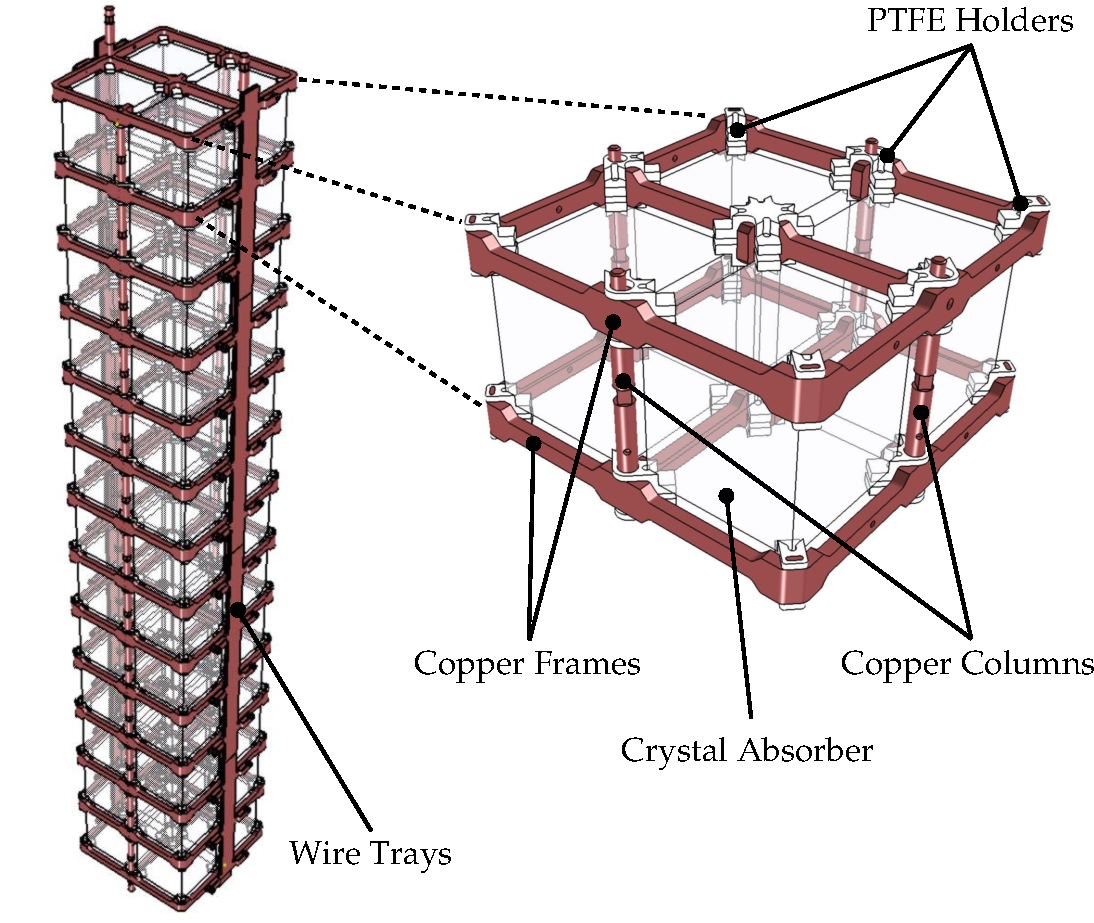
\includegraphics[width=0.8\linewidth]{Figures/fig02.pdf}
    \caption[A rendering of the components of a single CUORE tower (left) and floor (right).]
    {A rendering of the components of a CUORE tower (left) and floor (right).
    The copper frames are shared between floors, and only the PTFE and the gold wiring connecting the silicon heaters and NTD thermistors to the wiring on the frames act as the weak thermal contact to the detectors.
    Figure from \cite{Alduino:2016vjd}.}
    \label{fig:tower_rendering}
\end{figure}
It is important to note that the number and size of each component on the towers is minimized as much as possible, while keeping the structural integrity intact.
Since these components are the nearest to the detectors, keeping their radioactivity to a minimum significantly lowers the background and is discussed more in \autoref{ssec:CUORE-0}.
This was one of the improvements from Cuoricino's towers to CUORE's towers, as the amount of copper used in the frames was able to be reduced by a factor of $\sim2.5$.

As shown in \autoref{fig:tower_rendering}, there are trays on opposite sides of the tower.
These wire trays contain copper-insulator tape with a polyethylene naphthalate substrate (referred to as ``Cu-PEN" tape) and are used to electrically connect the NTD thermistors and the Si heaters on the detectors to the other NbTi cabbles that connect to the electronics at the top of the cryostat.
These cables have a length of 1.4 meters with a thickness of 80 $\mu \textrm{m}$ and a pattern of traces in the 17 $\mu \textrm{m}$ thick copper layer.
As the detectors are read out through these connections, they must have low cross-talk and microphonic pickup in addition to their background requirements.
Two sets of these cables are connected to two opposing sides of the towers, and branch out to connect to crystals on each floor.
These tapes  are divided into 4 types, depending on how far down along the tower they reach, and a separate tape is used for the Si heaters.
A photograph of these tapes is shown in \autoref{fig:CuPEN}.

\begin{figure}
    \centering
    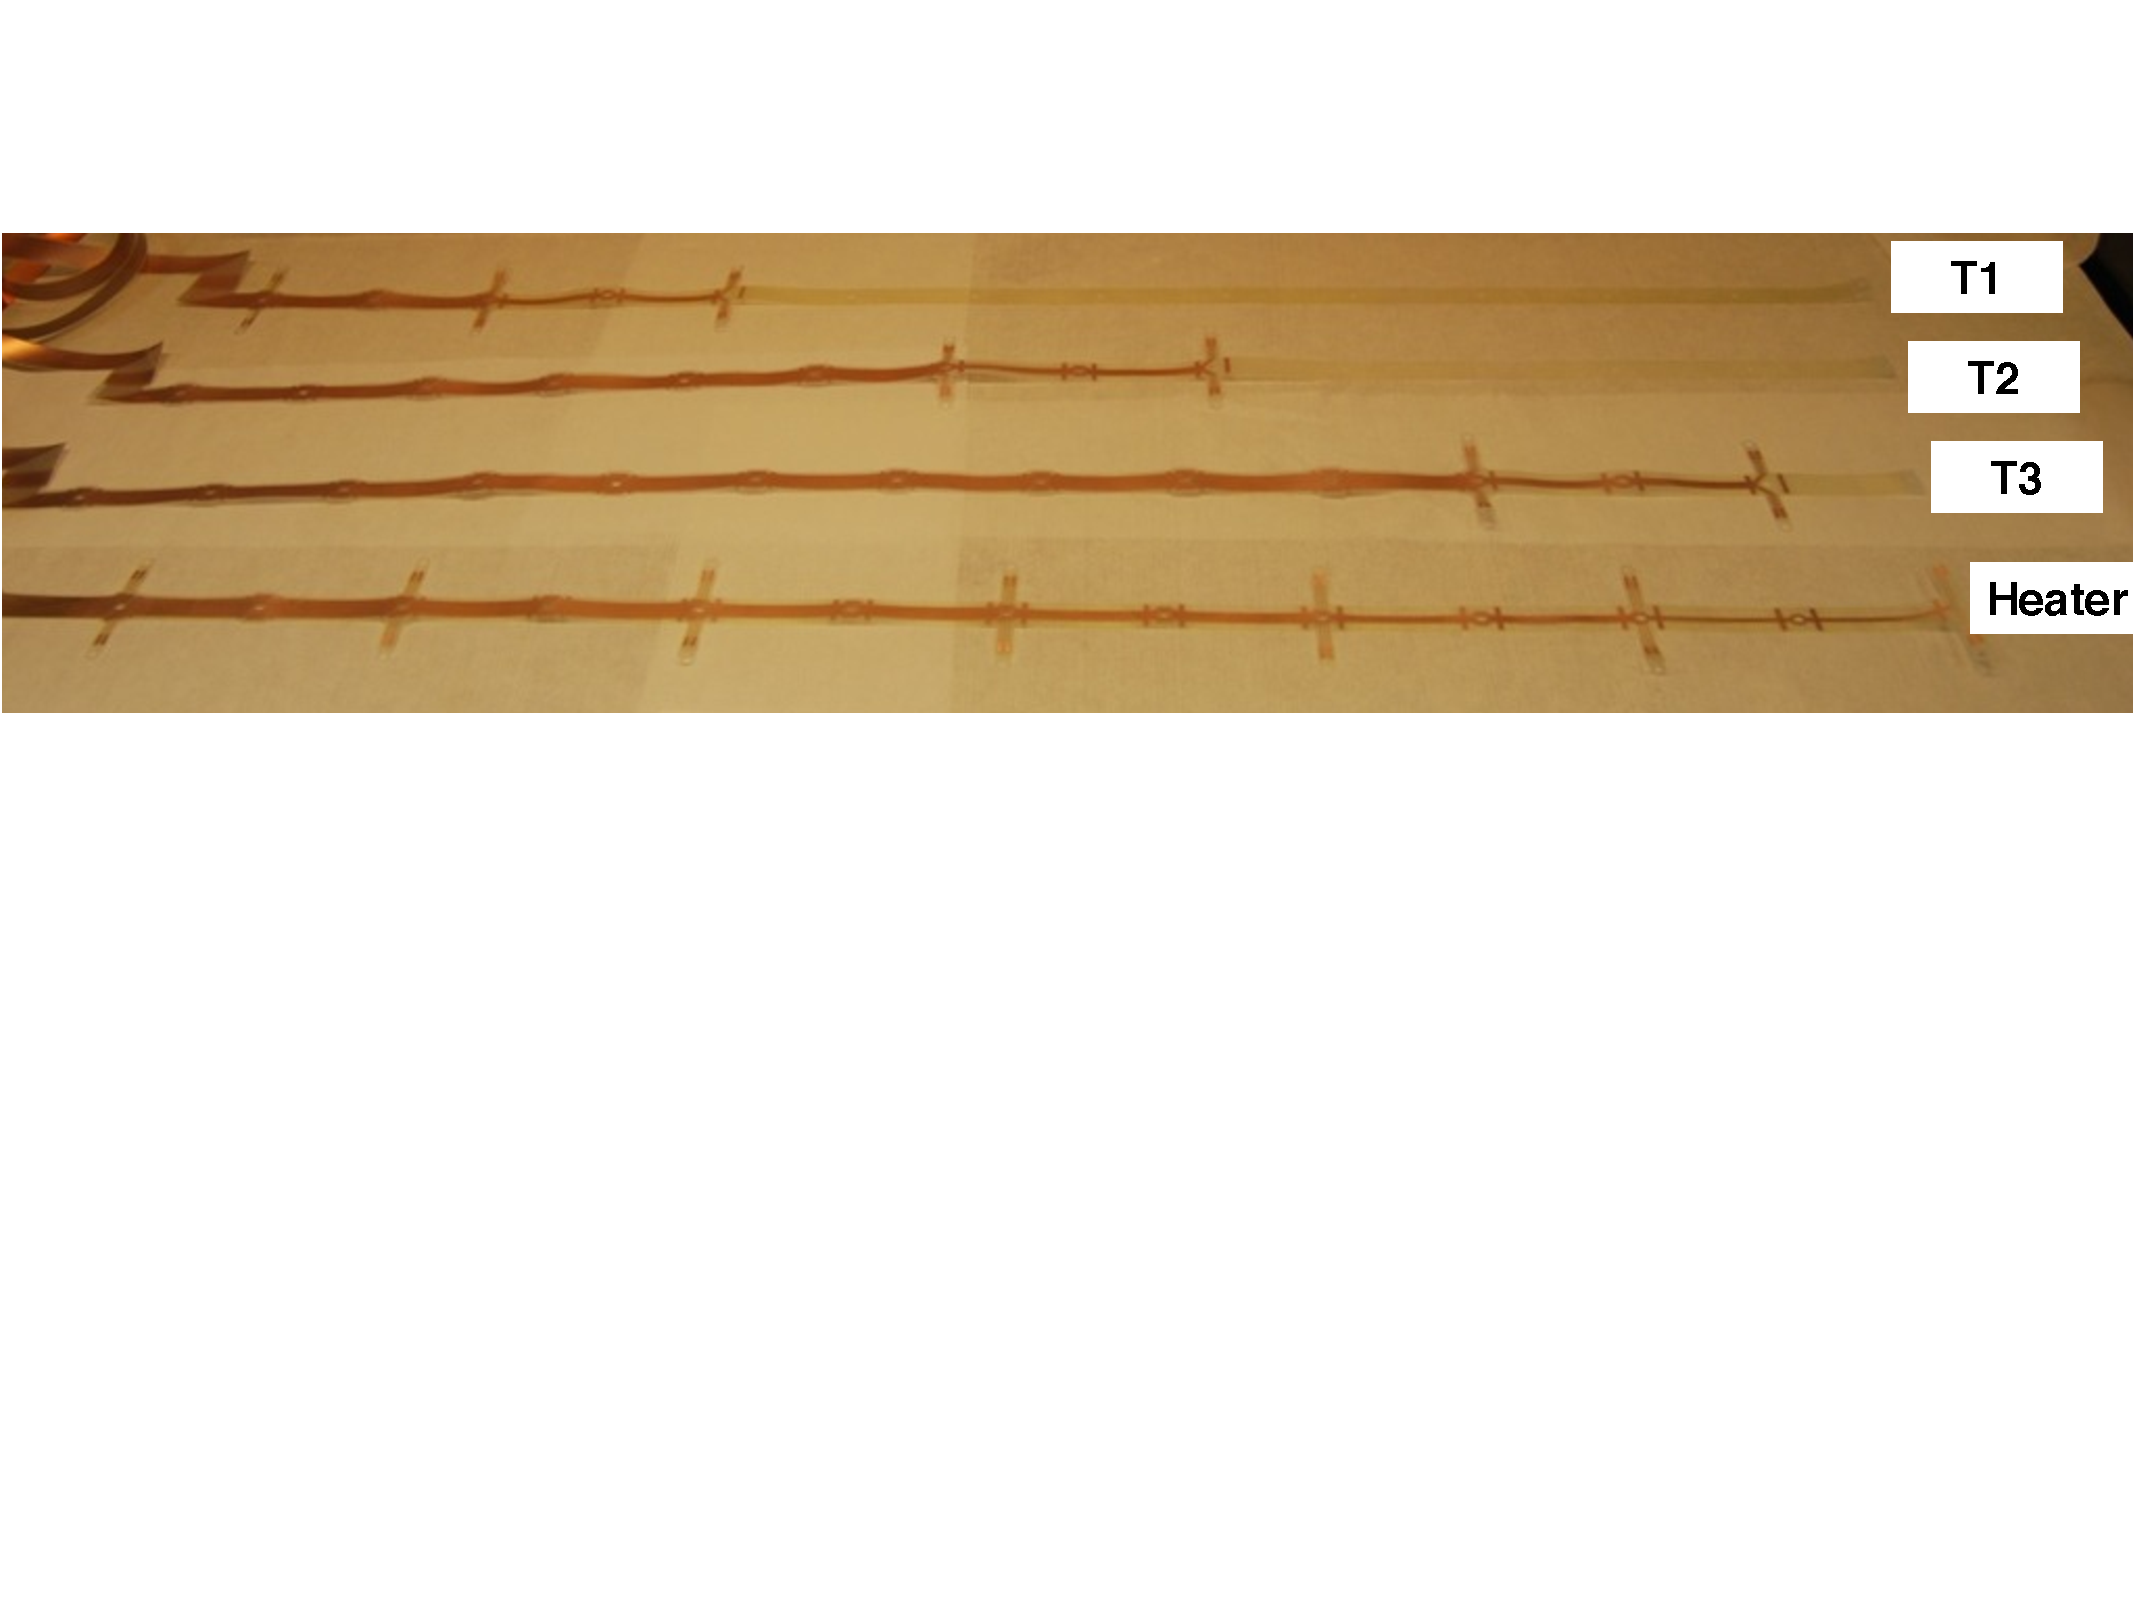
\includegraphics[width=0.9\linewidth]{Figures/fig07.pdf}
    \caption[A photograph of the Cu-PEN tapes that are placed inside the wire trays on the CUORE towers.]
    {A photograph of the Cu-PEN tapes that are placed inside the wire trays on the CUORE towers.
    The numbered tapes connect to floors 9-13, 5-8, and 1-4, respectively counting from the bottom of the tower, and the Heater tape contains two sets of signals to connect to a single column each.
    Figure from \cite{Alduino:2016vtd}.}
    \label{fig:CuPEN}
\end{figure}

\subsection{CUORE Tower Construction and Assembly}

\subsubsection{Crystal Growth}
As mentioned in the preceeding section, the first part of the detector construction and tower assembly occurrs with growth of the Te crystals at SICCAS.
This growth was performed in two phases: crystal growth and crystal polishing.
During each procedure, extreme care was taken to minimize bulk contaminations forming in the first phase and surface contaminations in the second \cite{crystal_growth_methods, crystal_growth_methods_2, Barghouty:2010kj}.
During the first procedure, the crystals are grown twice, where, after the first growth, 1 mm is removed from the ingots and the selected best sections of the first growth are used as high-purity powder for the second.
This two-stage growth process enables crystal purity of 99.999\%, up from the 99.99\% purity of commercially available powder.
This increased purity, along with growing the crystals from powder, strongly reduces bulk contaminations of $^{40}$K, which is a particularly problematic background for \twonubb~measurements, as it decays through beta-decay.

After the crystals are grown, they are then cut into cubes with $5 \pm 0.0050$ cm edges and $0.05$ cm chamfers with an average flatness on each face of $<0.001$ cm.
In addition, the cubic faces are oriented parallel to the planes of the crystalline structure of the \teotwo~within $\pm1^{\circ}$ by means of an X-ray on the crystals after their growth.
The cleaning process then takes two steps: first, by means of chemical etching, and, second, by polishing the crystals.
Each of these processes removes approximately $10^5$ atomic layers from the surface of the crystal, which removes surface impurities that may have adsorbed onto the crystal surface and begun to diffuse into the bulk.
At the end of the polishing step, the completed crystal is then triple-bagged in vacuum and stored in groups of 6 in a polyethylene vacuum box in order to avoid exposure to atmospheric radon.

Once the crystals arrive at LNGS, they are immediately placed in storage underground under a flux of nitrogen.
Despite the short $\sim$1 month that the crystals are aboveground causes the crystals to have cosmogenic activation of $^{110m}$Ag and $^{60}$Co that contribute $<1\%$ of the background at the Q-value of $^{130}$Te \cite{PhysRevC.92.024620, BARGHOUTY201316}.

\subsubsection{Parts Selection and Cleaning}
\label{ssec:Parts Selection and Cleaning}
The copper used to house the detectors in the detector array also undergoes an extensive cleaning process.
The copper selected for this is produced by Arubis\footnote{Originally named Norddeutsche Affinerie.} and is their high-purity Electrolytic Tough Pitch (ETP1) copper alloy, called NOSV\footnote{\RaggedRight\url{http://www.aurubis.com/en/our-business/products/aurubis-shapes/materials/shapes-materials-table}}.
This copper was chosen for CUORE due to its radiopurity and its high residual resistance ratio, certified to be over 400.
However, while the bulk contamination of NOSV copper is low, the surface contaminations of commercially-available NOSV copper due to its handling and machining.
This required the development of a stringent cleaning procedure that involved a sequence of tumbling and chemical etching.
In addition, the larger copper shields facing the detector were wrapped in polyethlyene film while the small copper parts on the towers were also subjected to Magnetron plasma etching, TECM.
This cleaning procedure required the copper to be above ground for a total of 4 months between casting and storage underground.
During this time, the cosmogenic activity for CUORE data-taking is estimated to be a negligible value of <50 $\mu$Bq$/$kg.
These procedures were validated during the Three Towers Test  and the surface contamination of the cleaned NOSV copper was measured to be 3.8 nBq/cm$^2$ and 2.0 nBq/cm$^2$ for $^{238}$U and $^{232}$Th, respectively \cite{ALESSANDRIA201313}.
The other components on the CUORE towers, viz. the NTDs, the silicon heaters, PTFE holders, etc., are also subjected to a cleaning process and are stored under a nitrogen flux before assembly.
The final bulk and surface contaminations of the components of the CUORE tower are shown in \autoref{tab:NearDetectorSources_Bulk} and \autoref{tab:NearDetectorSources_Surface}, respectively.

\begin{table}[htbp]
\centering
\caption[90\% C.L. upper limits of $^{232}$Th and $^{238}$U bulk contamination of sources near the detector.]
{90\% upper limits of $^{232}$Th and $^{238}$U bulk contamination of sources near the detector.
Table from \cite{Alduino:2017qet}.}
\label{tab:NearDetectorSources_Bulk}
\begin{tabular}{lll}
\hline
\hline
Material         & $^{232}$Th [Bq/kg]         & $^{238}$U [Bq/kg]    \\
\hline
TeO2             & $<8.4\times10^{-7}$ & $<6.7\times10^{-7}$      \\
Glue             & $<8.9\times10^{-4}$ & $<1.0\times10^{-2}$          \\
Au bonding wires & $<4.1\times10^{-2}$ & $<1.2\times10^{-2}$       \\
Si heaters       & $<3.3\times10^{-4}$ & $<2.1\times10^{-3}$        \\
NTDs             & $<4.1\times10^{-3}$ & $<1.2\times10^{-2}$    \\
Cu-PEN           & $<1.0\times10^{-3}$ & $<1.3\times10^{-3}$ \\
PTFE             & $<6.1\times10^{-6}$ & $<2.2\times10^{-5}$       \\
Cu NOSV           & $<2.1\times10^{-6}$ & $<6.5\times10^{-5}$    \\
\hline
\hline
\end{tabular}
\end{table}

\begin{table}[htbp]
\centering
\caption[90\% C.L. upper limits of $^{232}$Th, $^{238}$U, and $^{210}$Pb surface contamination and the contamination depth of sources near the detector.]
{90\% C.L. upper limits of $^{232}$Th, $^{238}$U, and $^{210}$Pb surface contamination and the contamination depth of sources near the detector.
Table from \cite{Alduino:2017qet}.}
\label{tab:NearDetectorSources_Surface}
\begin{tabular}{lllll}
\hline
\hline
Material         & Depth [$\mu$m] & $^{232}$Th [Bq/kg]         & $^{238}$U [Bq/kg]     & $^{210}$Pb [Bq/cm$^2$] \\
\hline
TeO2  & 0.01-10 & $<1.9\times10^{-9}$ & $<8.9\times10^{-9}$ & $<9.8\times10^{-7}$ \\
Si heaters  & 0.1-10 & $<3.3\times10^{-6}$ & $<8.2\times10^{-7}$ & $<8.2\times10^{-7}$ \\
NTDs  & 0.1-10 & $<8.0\times10^{-6}$ & $<5.0\times10^{-6}$ & $<4.0\times10^{-5}$ \\
Cu-PEN  & 0.1-30 & $<4.0\times10^{-6}$ & $<5.0\times10^{-6}$ & $<3.0\times10^{-5}$ \\
PTFE  & 0.1-30 & $<1.9\times10^{-8}$ & $<6.8\times10^{-8}$ & - \\
Cu NOSV & 0.1-10 & $<6.8\times10^{-8}$ & $<6.5\times10^{-8}$ & $<8.6\times10^{-7}$ \\
\hline
\hline
\end{tabular}
\end{table}

\subsubsection{Tower Assembly}
\label{ssec:Tower Assembly}
Assembling the towers components takes place in two stages.
First, a semi-automated workstation was set up to glue the NTD and Si heater chips to the crystals, and then another workstation with task-specific glove boxes for the assembly.
The activities were undertaken in a class 1000 (ISO 6) cleanroom in the same underground hut at LNGS as the CUORE cryostat.
During the entire assembly process, the tower materials are held in a nitrogen-flushed environment and contact with other materials is minimized to prevent contaminations.

For gluing the NTDs and Si heaters to the crystals, a six-axis articulated robotic arm lifts and positions the crystals, which are then glued by a three-axis Cartesian robot.
The glue dots are applied in the dot pattern shown in \autoref{fig:glue} as there is a mismatch between the thermal expansion coefficients for the components.
This pattern balances the need for good thermal coupling with the mechanical stress resulting from cooling down the crystals.
The use of a semi-automated system was learned from the experience in the Cuoricino experiment, where manual gluing strongly affected the signal shapes\footnote{Not to mention scaling up to 988 crystals in CUORE requires more uniformity and less manually-intensive labor per crystal/tower.}.
The setup used for the entire gluing process is shown in \autoref{fig:gluing_workstation}.

\begin{figure}[htbp]
    \centering
    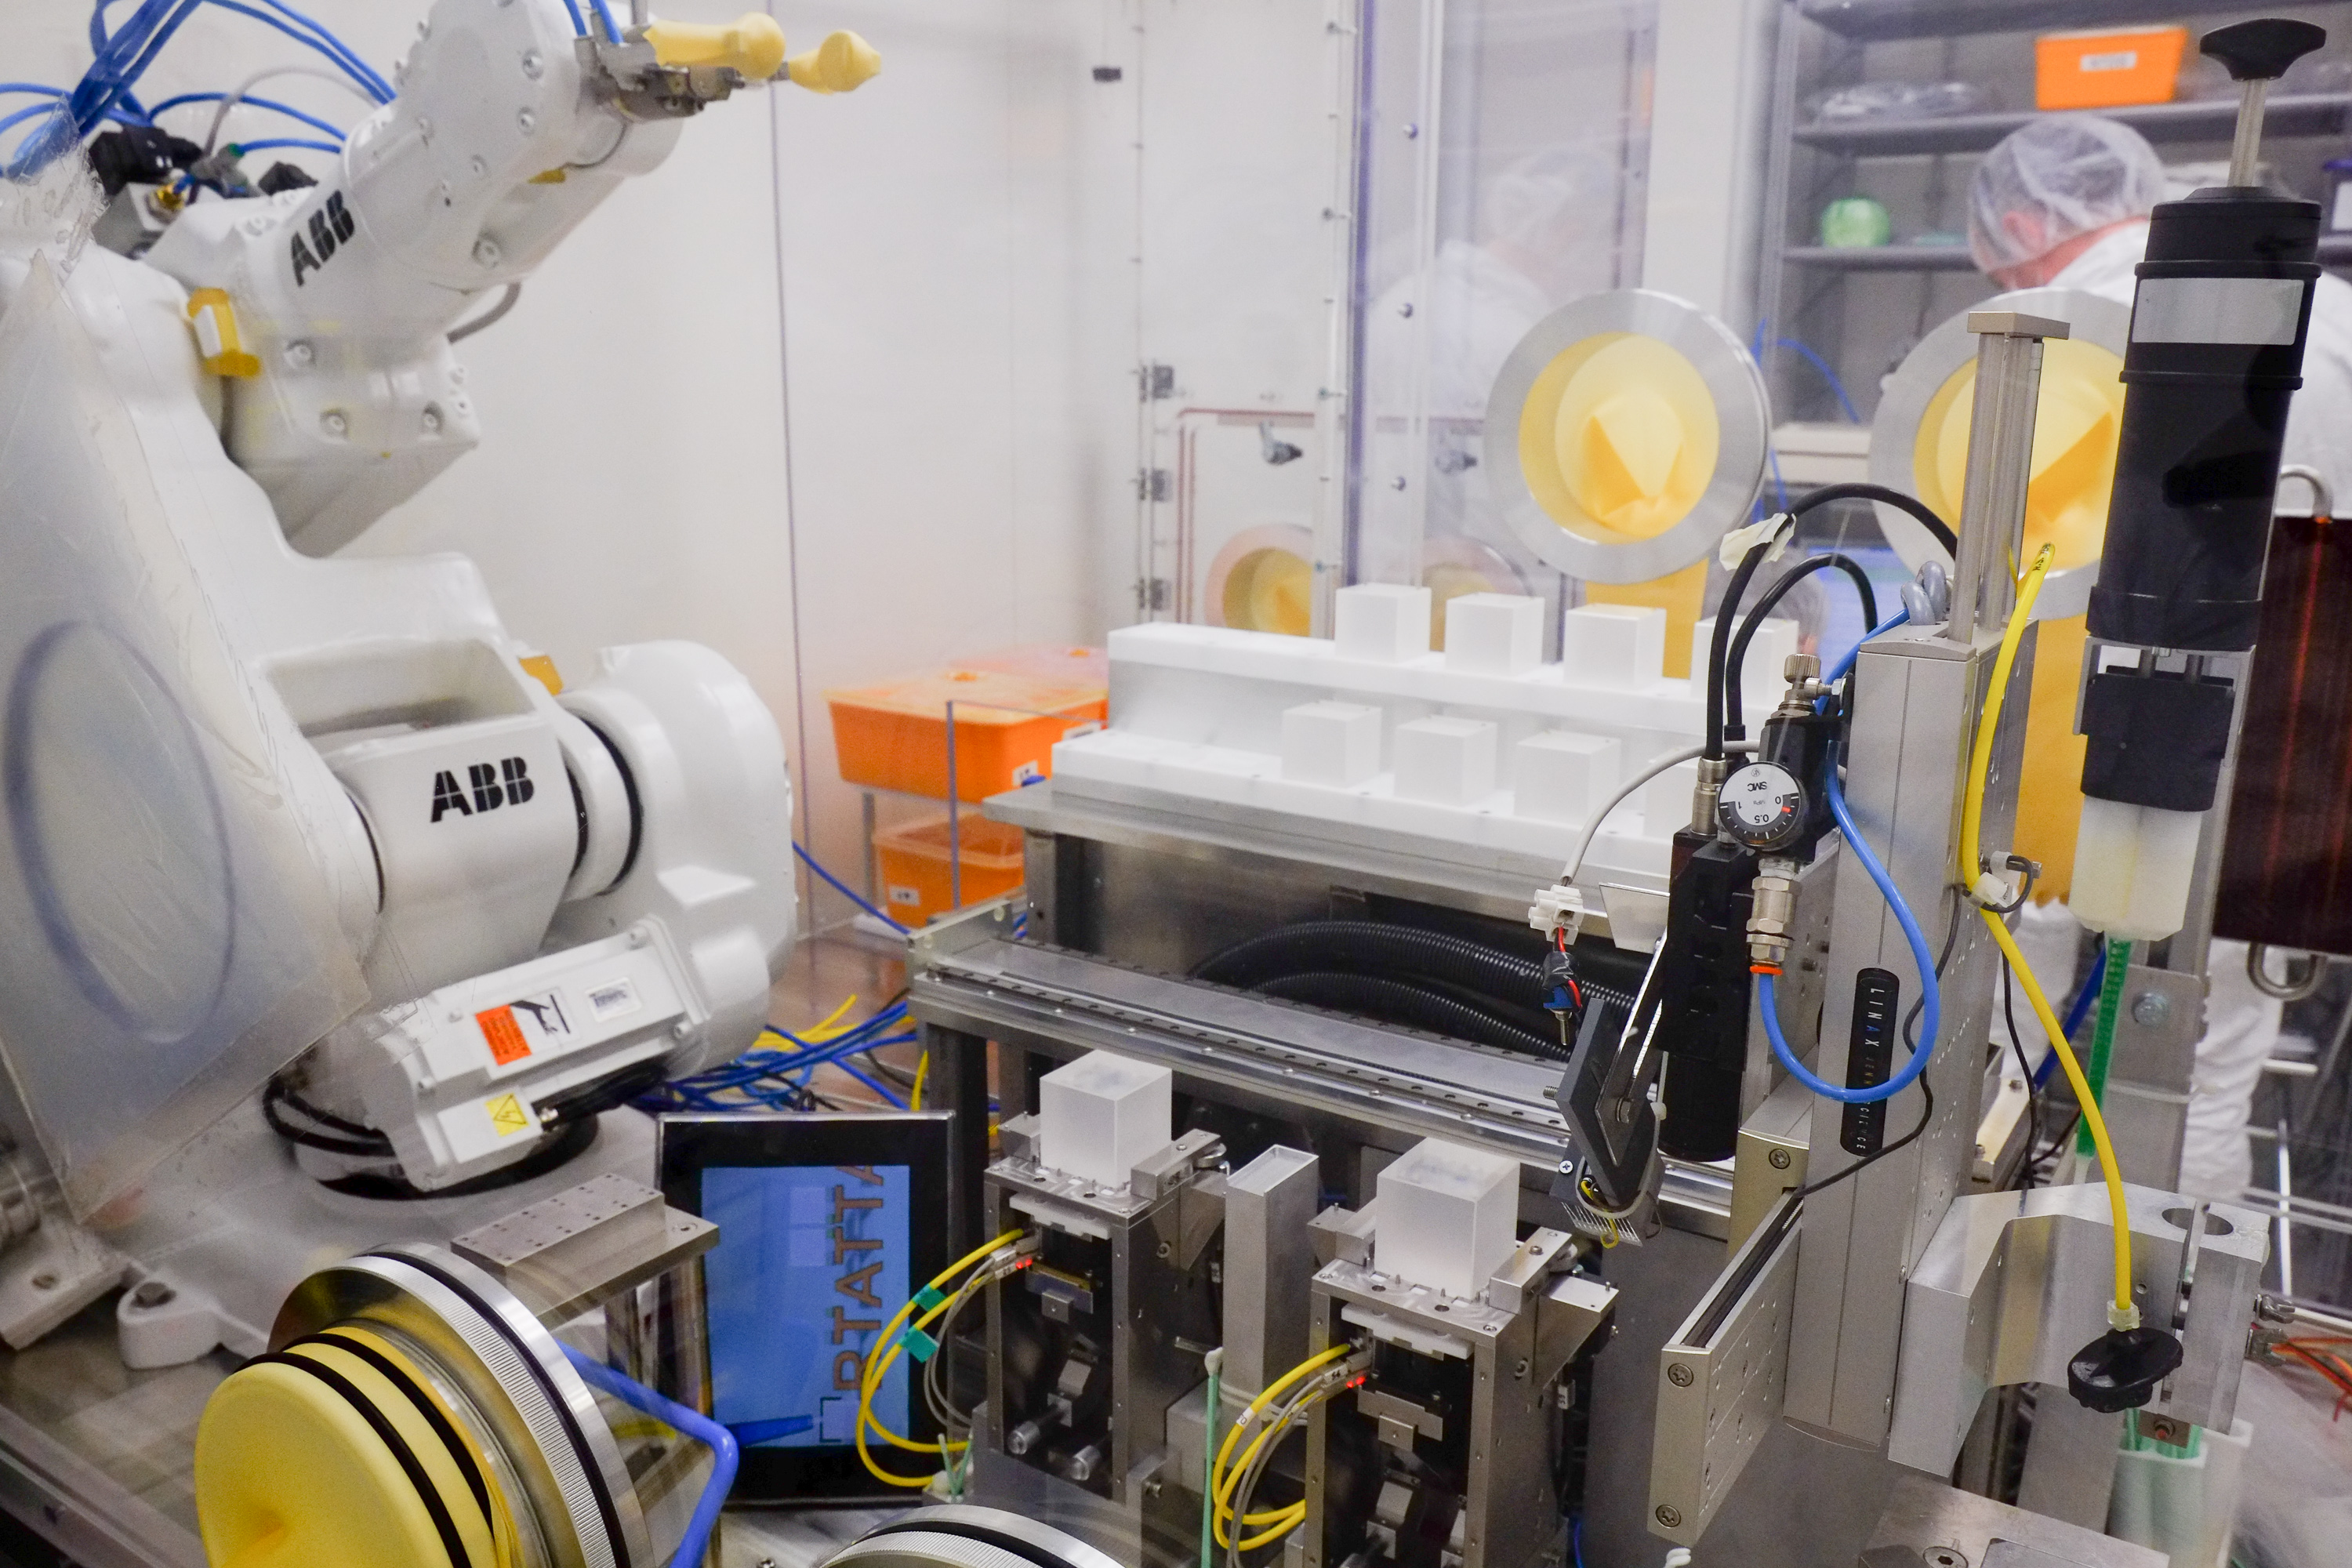
\includegraphics[width=0.7\linewidth]{Figures/cuore_gluing_pic1.jpg}
    \caption[The CUORE gluing workstation.]
    {The CUORE gluing workstation.
    On the left, the robotic arm lifts and moves the crystals, which can be seen on the workstation in the center, as needed for the gluing process.
    The Cartesian robot is on the right side of the workstation, along with the glue mixer.
    Photograph courtesy of the CUORE collaboration.}
    \label{fig:gluing_workstation}
\end{figure}

In the gluing process, the NTD thermistor and Si heater are placed upside down and then the mixed epoxy is injected into a syringe on the Cartesian robot and deposited onto the chips.
After the dots are inspected, a crystal is then taken from the shelf and placed above the chips with a hard face of the crystal facing the chips.
During this time, vacuum suction is used to keep the crystals at a distance of 50$\pm 5~\mu$m from the chips.
This whole process takes three minutes, taking into account the setting time of the epoxy.
After the crystal is glued, allowing as a precaution an hour for the epoxy to cure, the glued crystals are then removed from the glove box inside a vacuum-sealed box and placed into nitrogen-flushed storage.

After the gluing is completed, the assembly of the tower begins.
This is done at a separate workstation which consists of a ``garage" flushed with nitrogen to store the tower and a specialized glovebox that can couple to the garage depending on the task at hand.
First, the assembly takes place one floor at a time, with the crystals being placed in the teflon supports in the NOSV coper structure.
This assembly is shown in \autoref{fig:assemblybox}.

\begin{figure}[htbp]
    \centering
    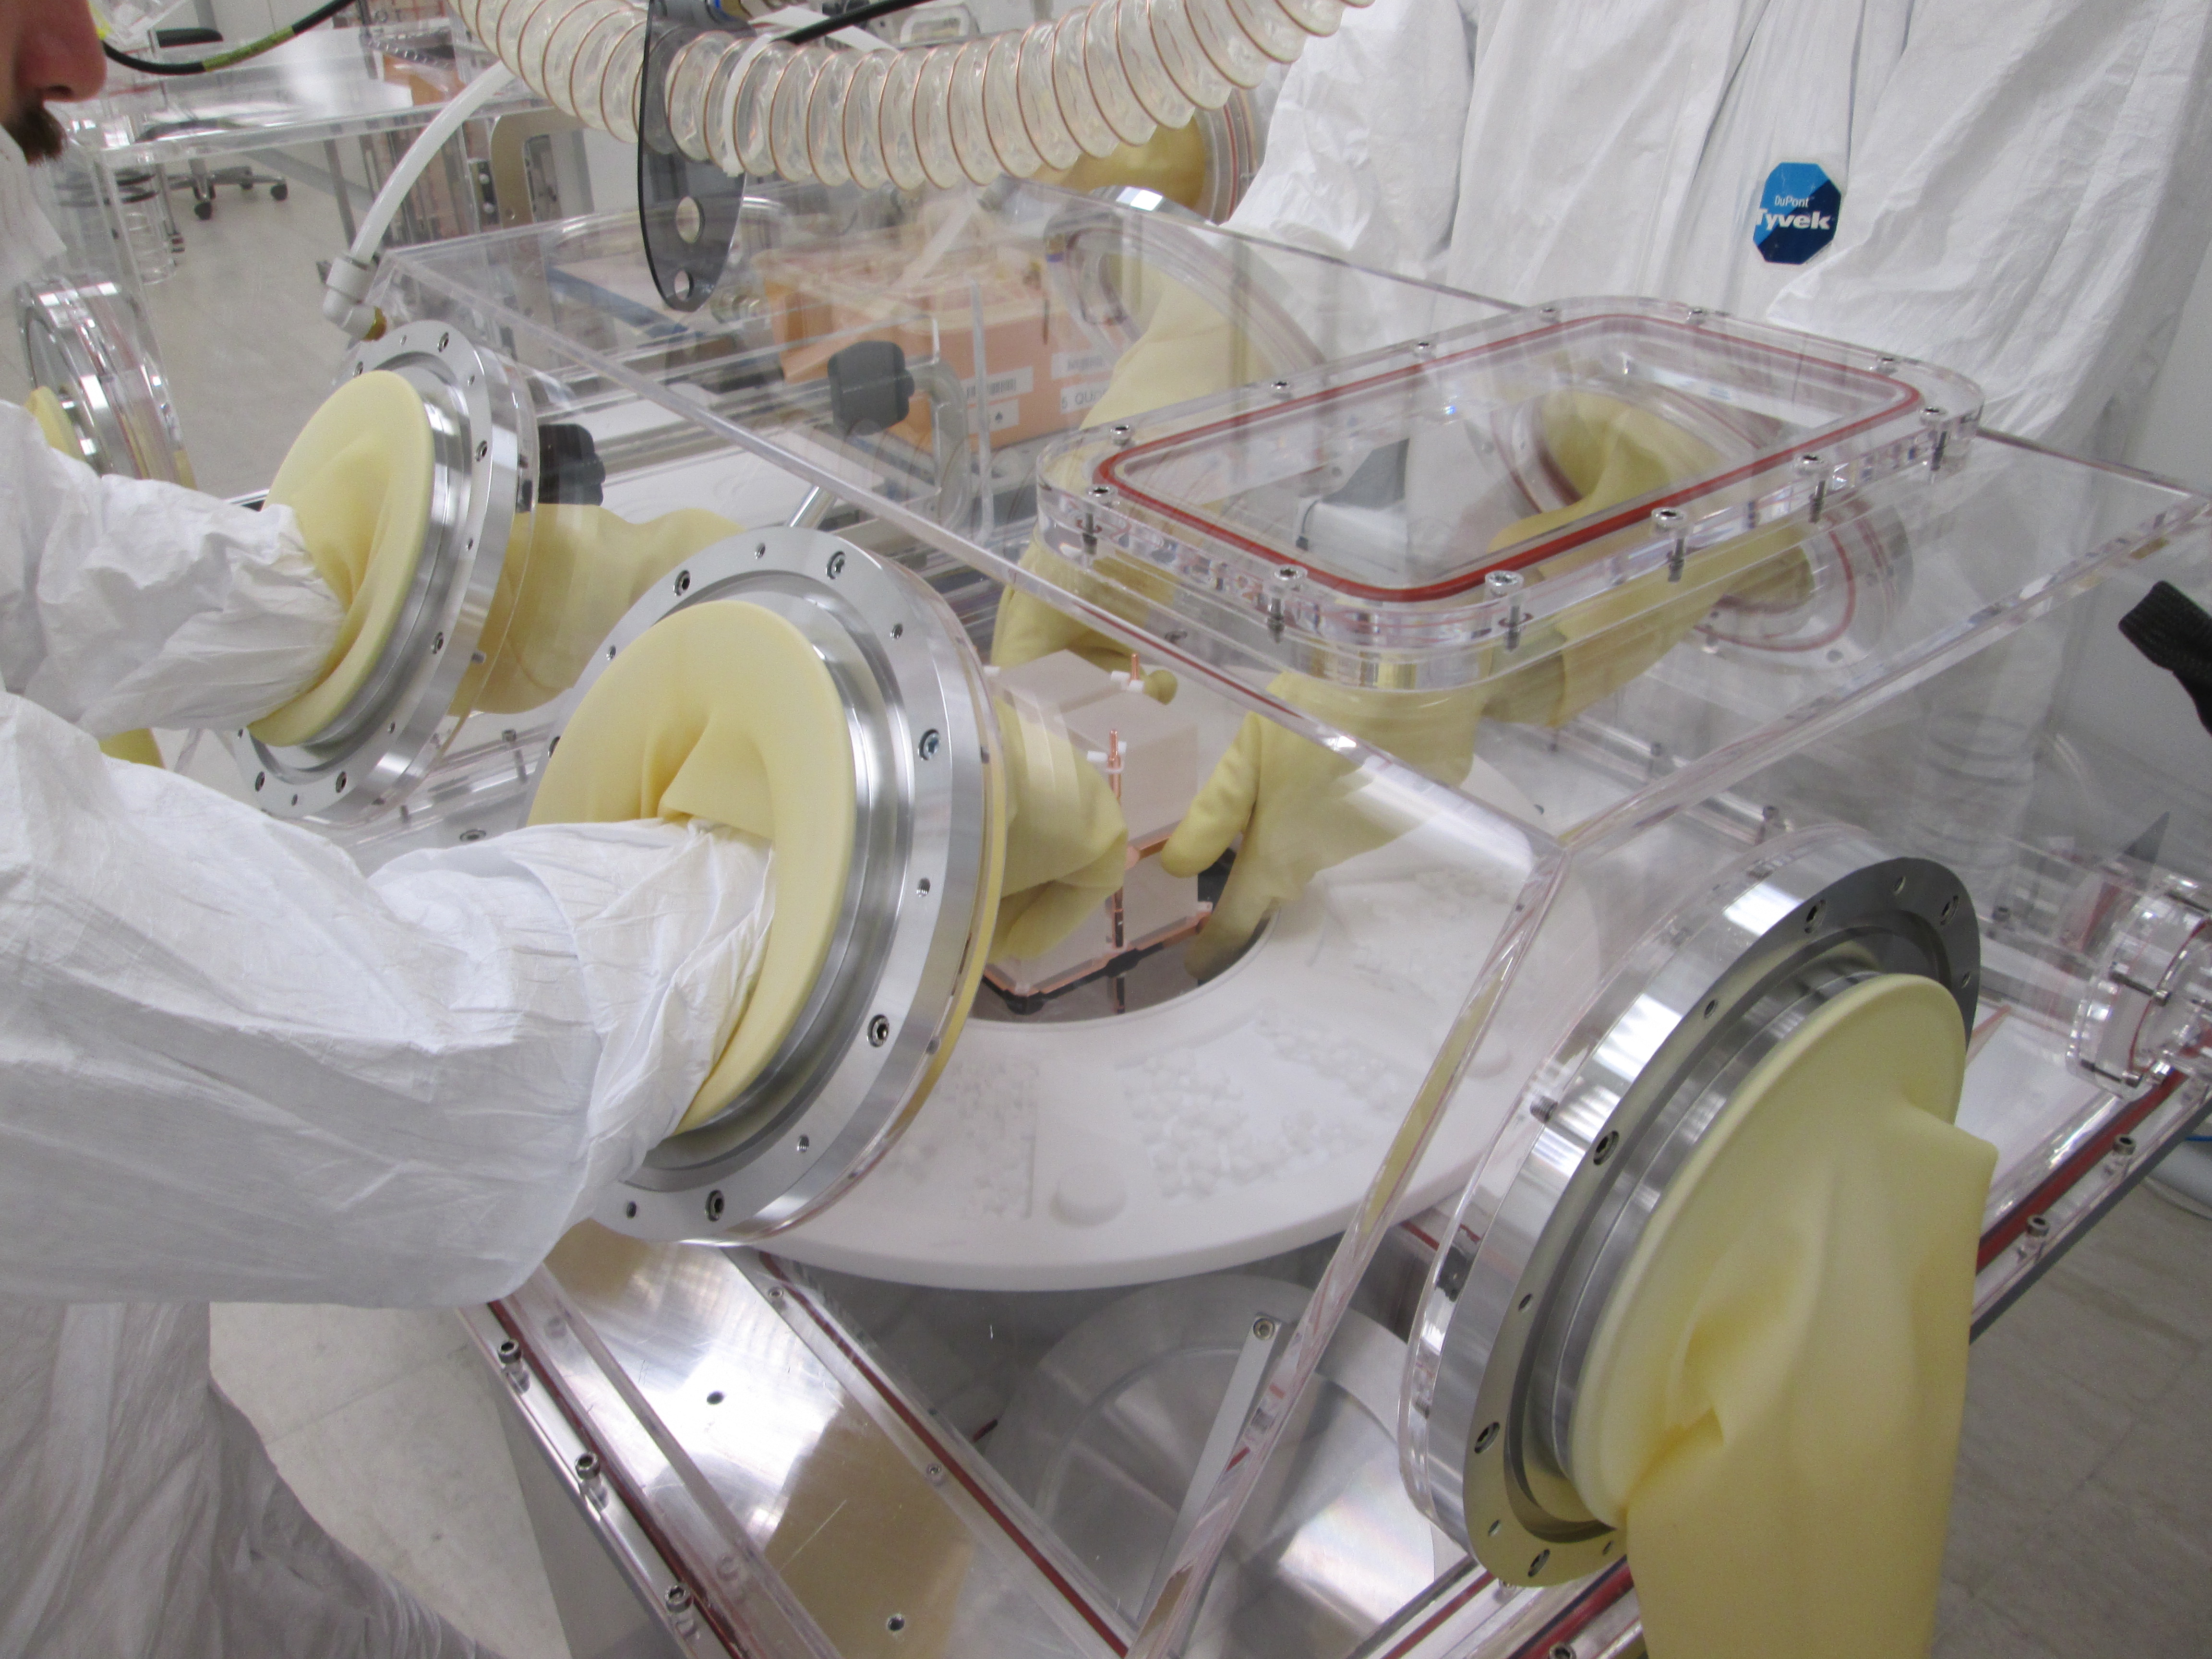
\includegraphics[width=0.6\linewidth]{Figures/TowerAssemblyBox.jpg}
    \caption[The glovebox used for tower assembly.]
    {The glovebox used for tower assembly.
    As each floor of the tower is completed, the tower is lowered into the garage.
    Once all 13 floors are assembled, the tower is sealed into the garage and the next glovebox is put into place above.
    Photograph courtesy of the CUORE collaboration.}
    \label{fig:assemblybox}
\end{figure}

The next part of the assembly is to attach the CuPEN tapes to the sides of the tower inside a larger glovebox.
The tapes are glued to the wire trays by means of Araldite Standard bicomponent epoxy\footnote{\RaggedRight\url{http://www.go-araldite.com/products/epoxy-adhesives/araldite-standard-2-x-15ml-tube}}.
The glovebox used for this procedure is shown in \autoref{fig:assemblybox_2}.
The wire trays are left open until the next step, the wire bonding of the chips to CuPEN tape, is completed.


\begin{figure}[htbp]
    \centering
    \includegraphics[width=0.6\linewidth, angle=90,origin=c]{Figures/TowerAssemblyBox_2.jpg}
    \caption[The assembly box used to assemble the CuPEN tapes on the towers.]
    {The assembly box used to assemble the CuPEN tapes on the towers.
    This assembly box is also flushed with nitrogen when a tower is in place, and the vertical access (in comparison with the box in \autoref{fig:assemblybox}) allows for placing the wire trays and tapes on the tower.
    The $\approx60~\textrm{cm}$ of tape is rolled up inside PTFE cylinders and can be seen at the top of the tower.
    Photograph courtesy of the CUORE collaboration.}
    \label{fig:assemblybox_2}
\end{figure}

The last step of the tower assembly process is the bonding of the gold wires to the copper pads on the tower.
This step is performed in the same glovebox as the previous step, but a modified Westbond 7700E manual wire bonder, mounted on rails and shown in \autoref{fig:bonding_machine}, is inserted on the right side of the glovebox.
With this bonder, the gold cables (4 for redundancy) are ball-bonded onto the chip pads and then wedge bonded to the copper pads on the CuPEN tape, as shown in \autoref{fig:bonds}.
Finally, another ball-bond is placed on the wedge bond to add extra security to the connection.
Considering the 988 crystals to be instrumented, and in line with the previous comments regarding the uniformity of the gluing, this process was also designed to be as repeatable as possible, and the lengths of the bonded gold wire are as uniform as possible.
After the tower assembly is completed, the towers are stored in nitrogen-flushed containers, shown in \autoref{fig:tower_storage}.

\begin{figure}[htbp]
    \centering
    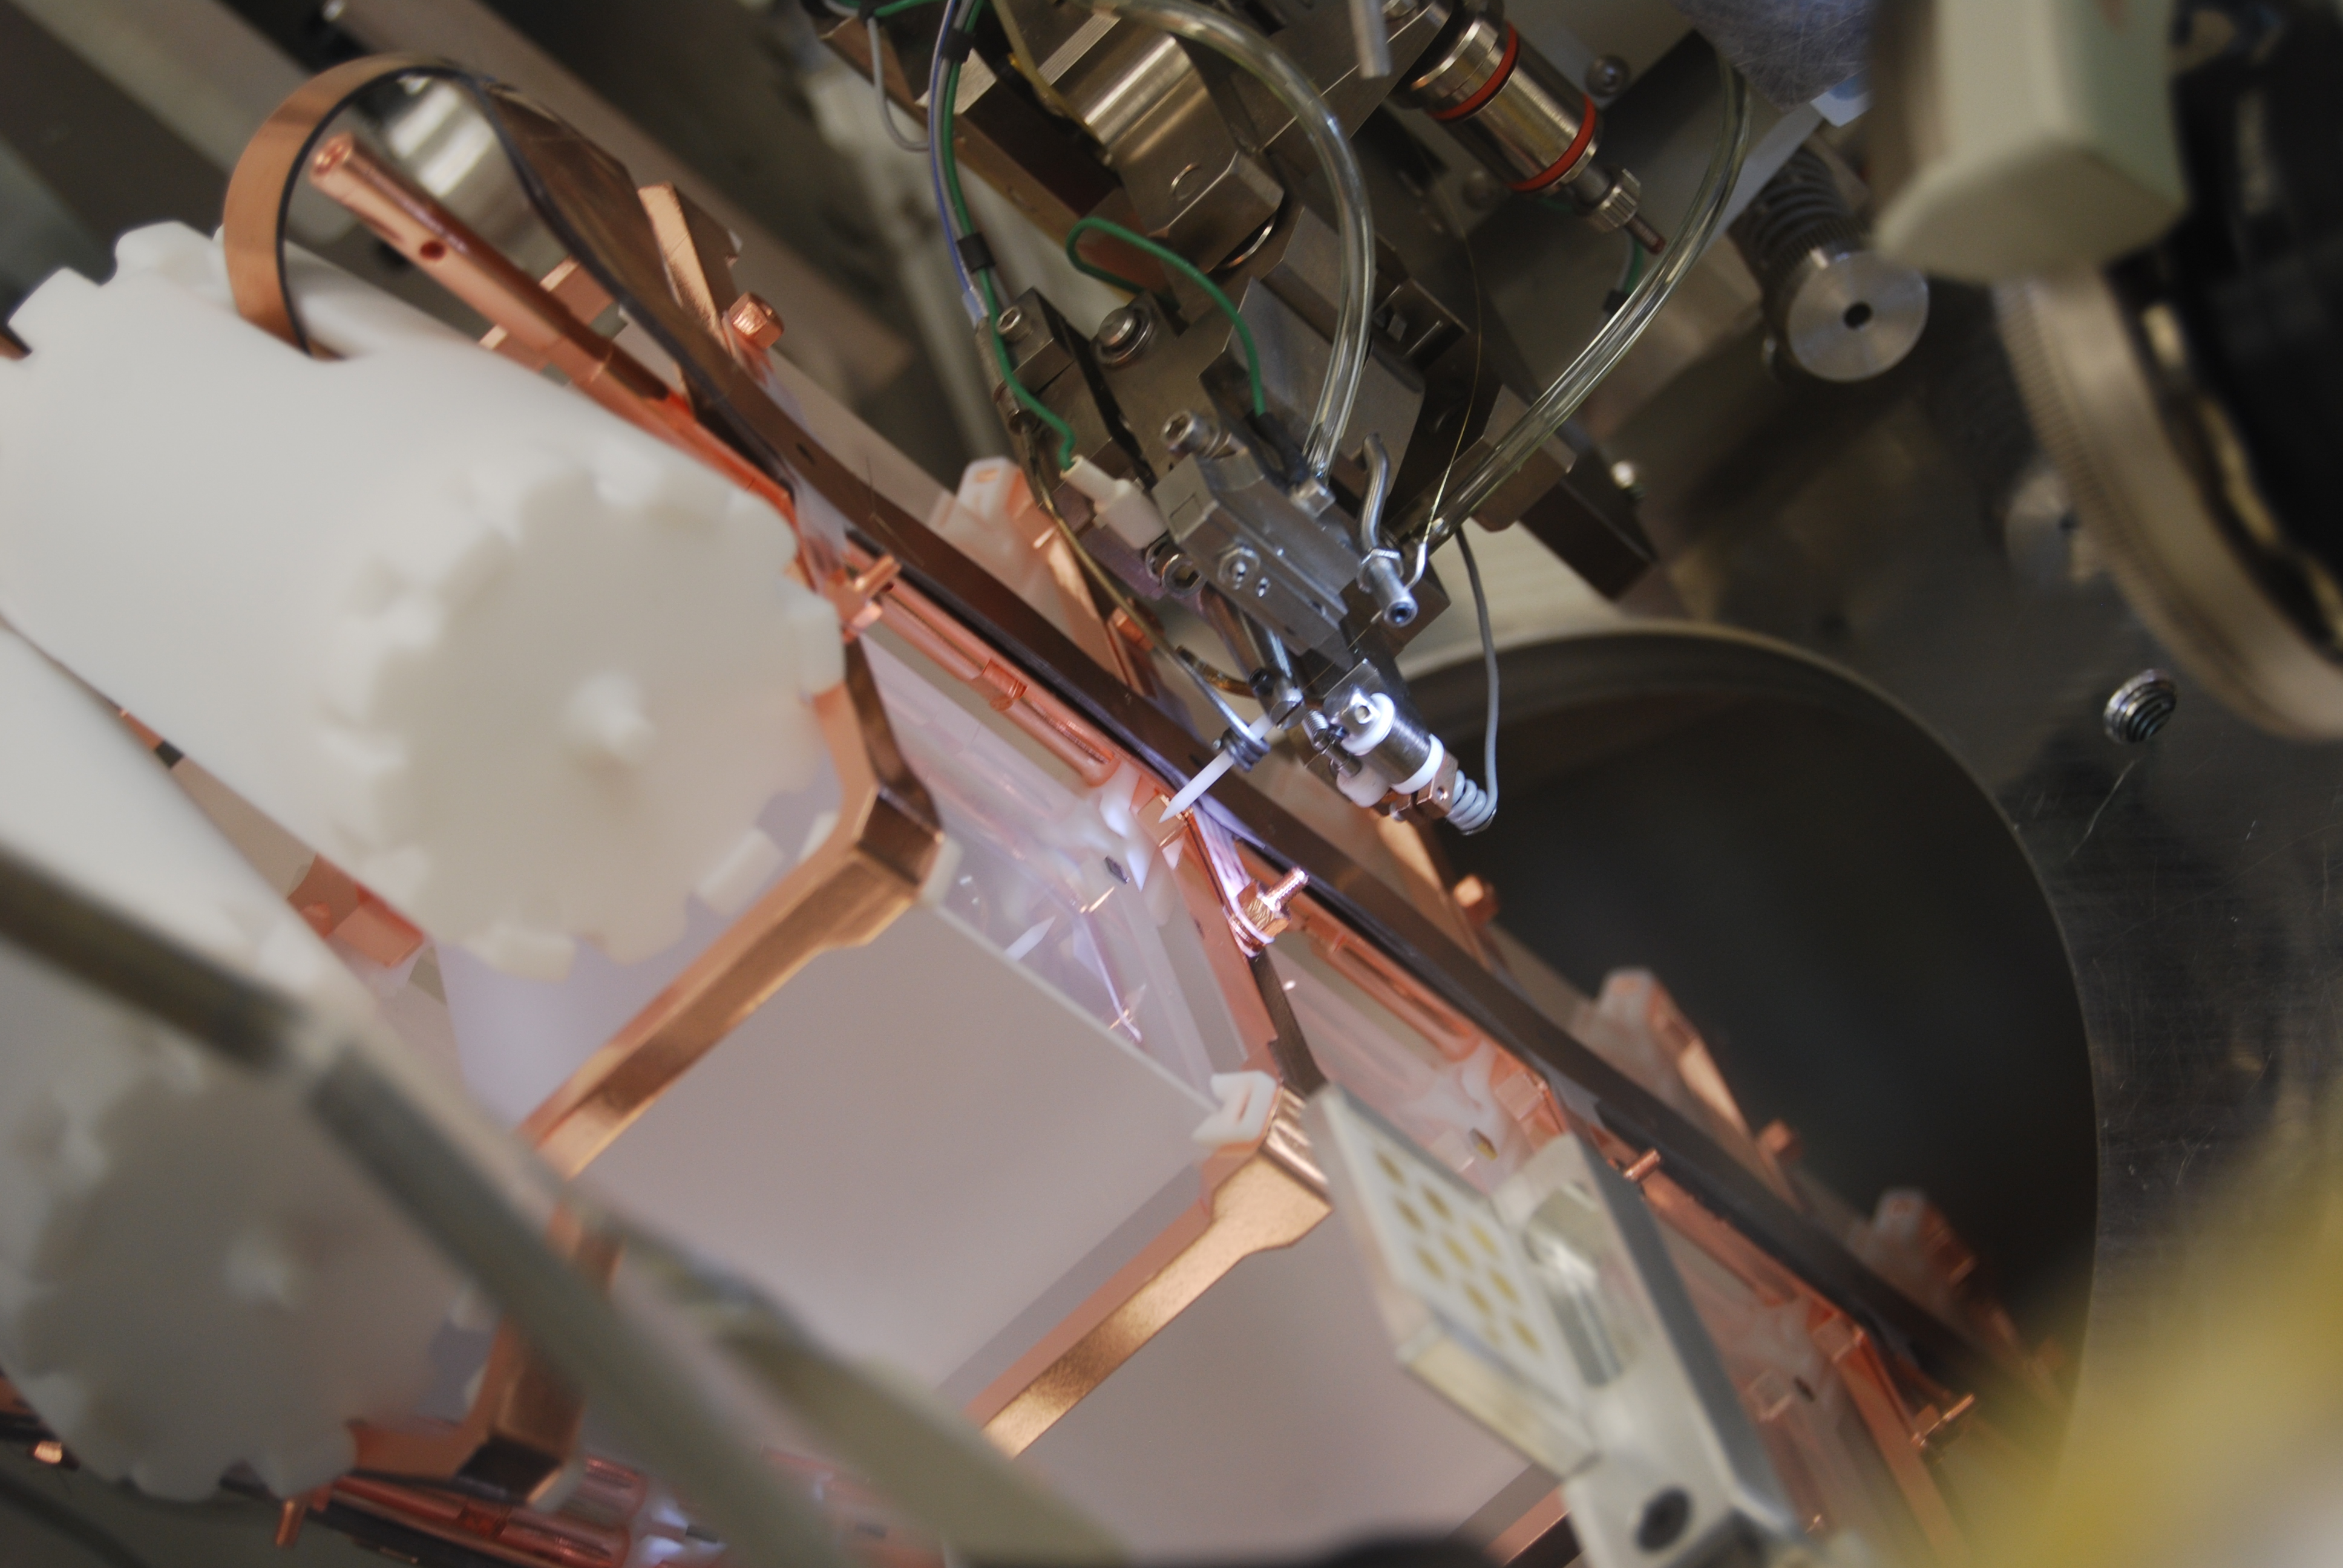
\includegraphics[width=0.6\linewidth, angle=270, origin=c]{Figures/bonding_machine.jpg}
    \caption[The wire bonding machine used in CUORE.]
    {The wire bonding machine used in CUORE.
    The bonder was modified to allow motion vertically and the rails serve to increase its reach.
    The tower is raised/lowered or rotated by a second operator, and a video camera with high magnification is used to make and verify the connections.
    Photograph courtesy of the CUORE collaboration.}
    \label{fig:bonding_machine}
\end{figure}

\begin{figure}[htbp]
    \centering
    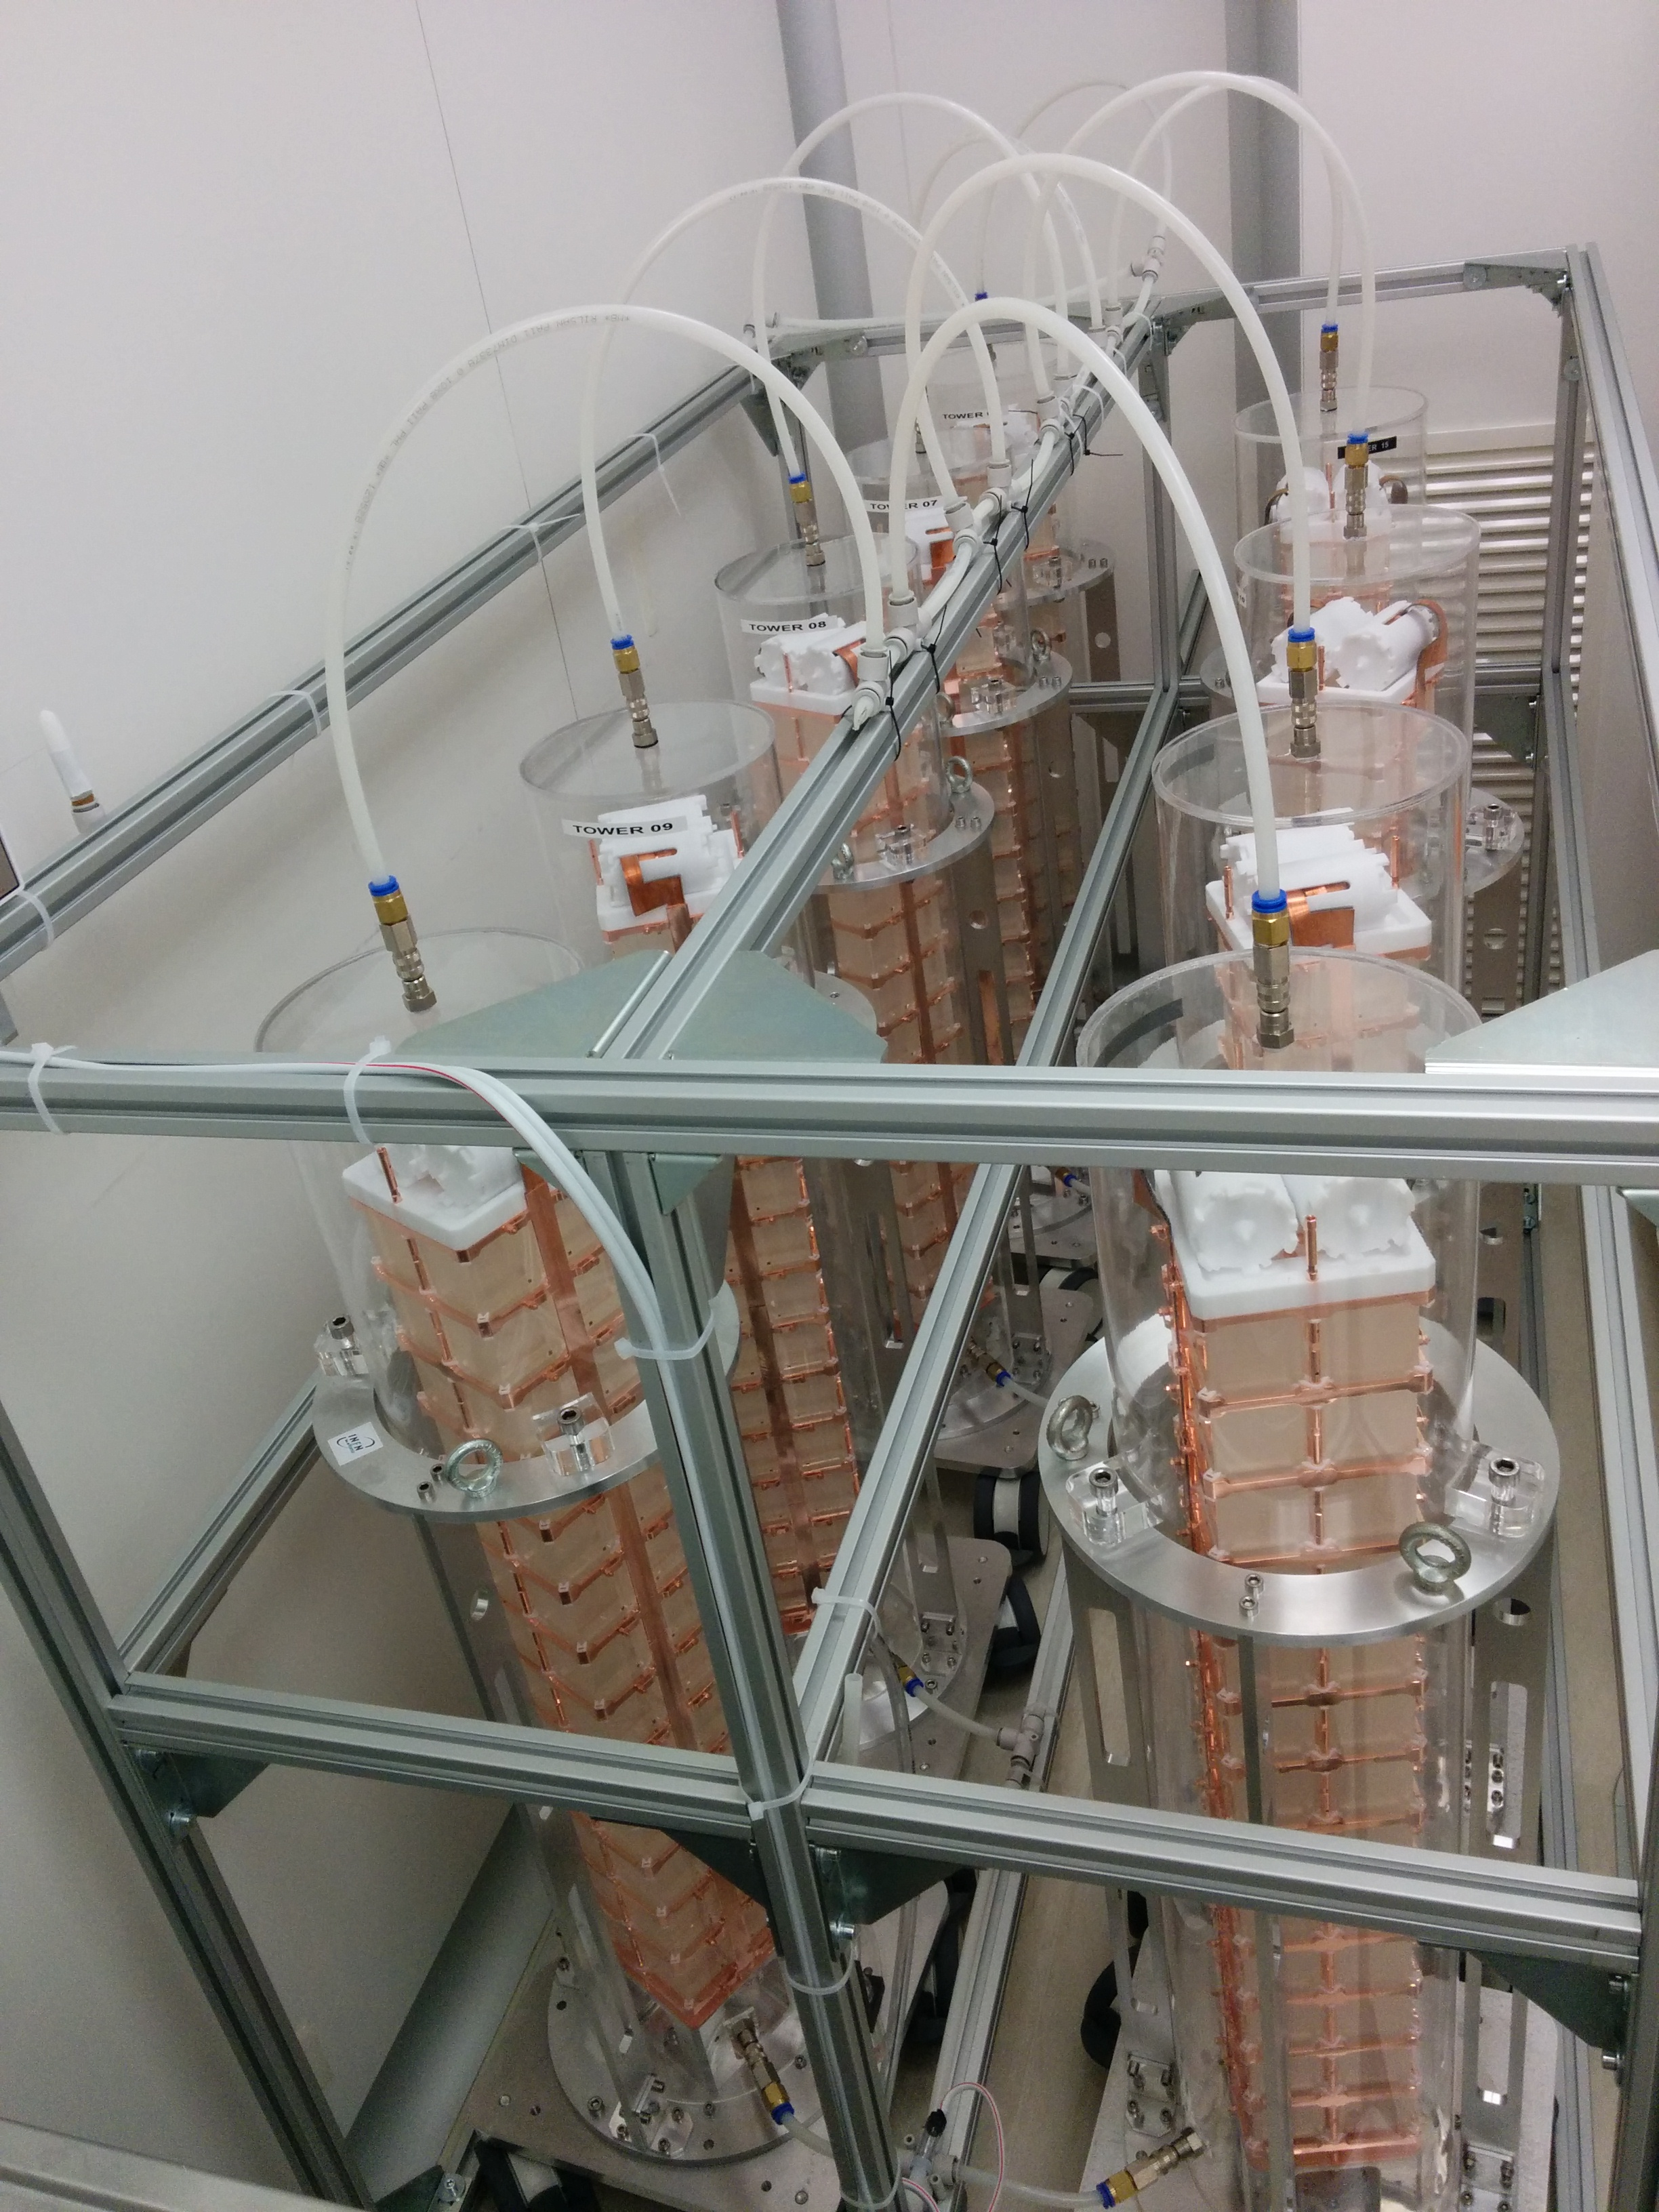
\includegraphics[width=0.5\linewidth]{Figures/cuore_towers_pic1.jpg}
    \caption[The storage area for the completed CUORE towers before installation.]
    {The storage area for the completed CUORE towers before installation.}
    \label{fig:tower_storage}
\end{figure}

\subsubsection{Tower Installation}
After the towers are completed and and the cryostat is ready for operation, the CUORE towers need to be installed into the cryostat.
This is another critical operation, as this is the first and only time that the CUORE crystals are exposed to air, with an approximate exposure of 1 day per tower.
In order to complete this activity, a specialized clean room was installed around the exposed inner part of the cryostat.
As the danger of being exposed to air is due to the presence of Radon in the air.
LNGS has an activity of 80 $\textrm{Bq}/\textrm{m}^3$ of Radon \cite{UndergroundLabs_Radon}, which required the use of a system to flush this specialized clean room with radon-free air.
This system reduced the radon to $<1~\textrm{Bq}/\textrm{m}^3$.
Each of the towers is then connected to the tower support plate independently, and the inner guide tubes for the DCS, discussed later in \autoref{chap:DCS}, are also connected at this time.
A view of the completed cryostat is shown in \autoref{fig:cuore_photograph}.


\begin{figure} [htbp]
    \centering
    \includegraphics[width=0.8\linewidth]{Figures/CUORE_29Aug16_HR-2477.jpg}
    \caption[A photograph of the 19 CUORE towers from below.
    Photo Credit: Yury Suvorov.]
    {A photograph of the 19 CUORE towers from below after installation in the cryostat.
    Also visible are the inner calibration source tubes with their PTFE caps.
    Photo Credit: Yury Suvorov.}
    \label{fig:cuore_photograph}
\end{figure}

\section{Predecessor Experiments}
\label{sec:Predecessor Experiments}
The CUORE experiment benefits from the experience gained through multiple previous incarnations of this bolometric technique in \teotwo.
Starting with the smallest proof-of-concept detectors, successive generations of this technology \cite{ }have increased in total detector mass and decreased in background in order to increase sensitivity and further probe \zeronubb~decay.
This almost-exponential growth in mass in the different generations of CUORE-like experiments from 73~g to 742~kg is shown in \autoref{fig:bolometer_mass_over_time}.
Of course, as shown in \autoref{eq:sensitivity_short}, the detector mass is only one part of the sensitivity equation, but successive experiments have also have significantly reduced backgrounds and other improvements to increase sensitivity beyond merely the increase from increased mass.
As a full description and history of the CUORE-like experiments is too long for discussion here, the most recent experiments, viz. Cuoricino and CUORE-0, that directly inform choices made for CUORE are described below.

\begin{figure}[htbp]
    \centering
    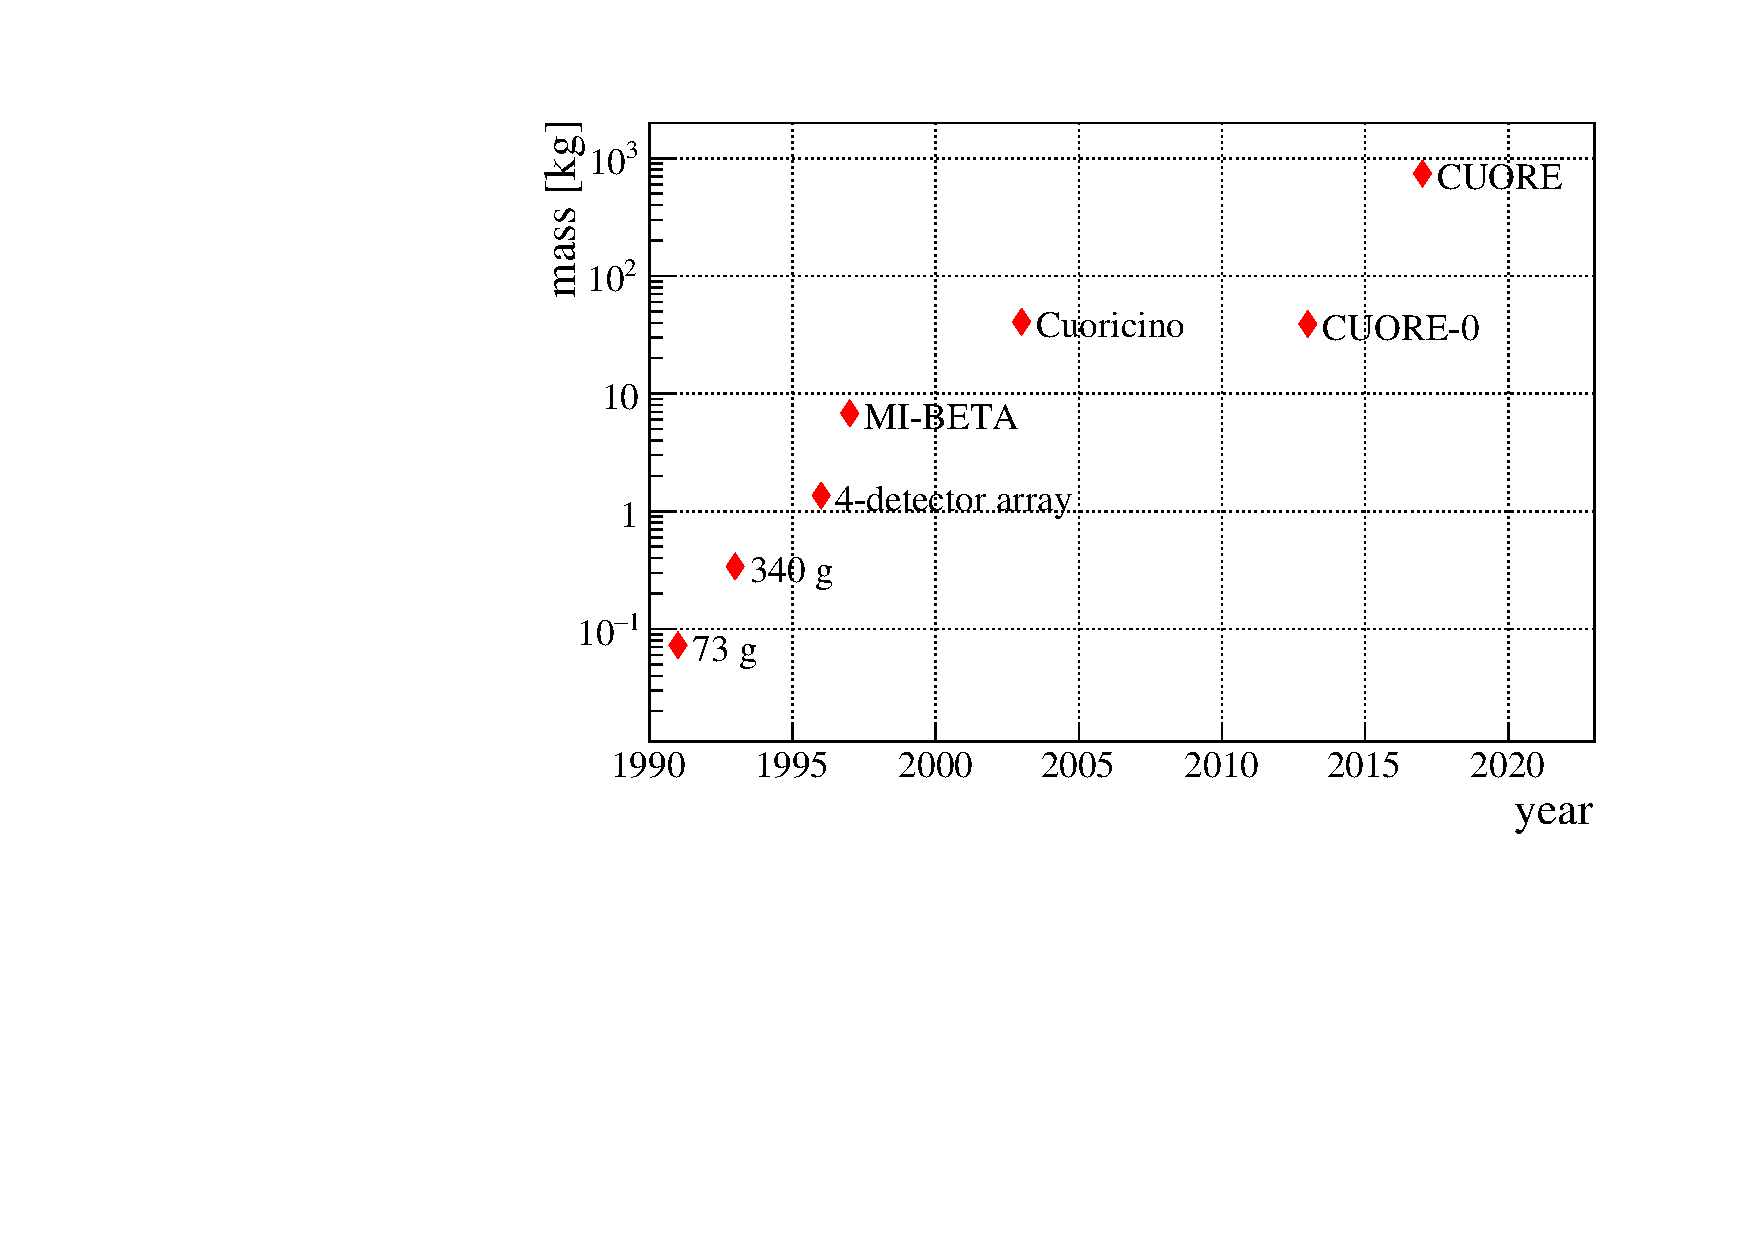
\includegraphics[width=\linewidth]{Figures/bolometer_mass_over_time.pdf}
    \caption[The increase in mass of \teotwo~crystals in successive experiments.]
    {The increase in mass of \teotwo~crystals in successive experiments.}
    \label{fig:bolometer_mass_over_time}
\end{figure}

\subsection{Cuoricino}
Building off the success of the Mi-Beta experiment \cite{Pirro:2002gw}, the Cuoricino experiment \cite{Andreotti:2010vj} performed a search of \zeronubb~with a tower consisting of 62 \teotwo~crystals, shown in \autoref{fig:Cuoricino_tower}, and, in addition, the Cuoricino experiment also served as a testing bed for CUORE.
Of the 62 crystals used in Cuoricino, 44 were ``big crystals" with $5\times5\times5~\textrm{cm}^3$ of naturally-abundant $^{130}$Te, 14 were ``small crystals" with $3\times3\times6~\textrm{cm}^3$ of naturally-abundant $^{130}$Te, 2 were the same size as the small crystals but with 75\% enriched $^{130}$Te, and the final 2 crystals were enriched with $^{128}$Te and had a negligible $^{130}$Te content.
In total, the crystals had a mass of $\approx11$ kg of $^{130}$Te and completed data-taking with 19.75 $\textrm{kg}\cdot \textrm{yr}$ of $^{130}$Te exposure.

\begin{figure}[htbp]
    \centering
    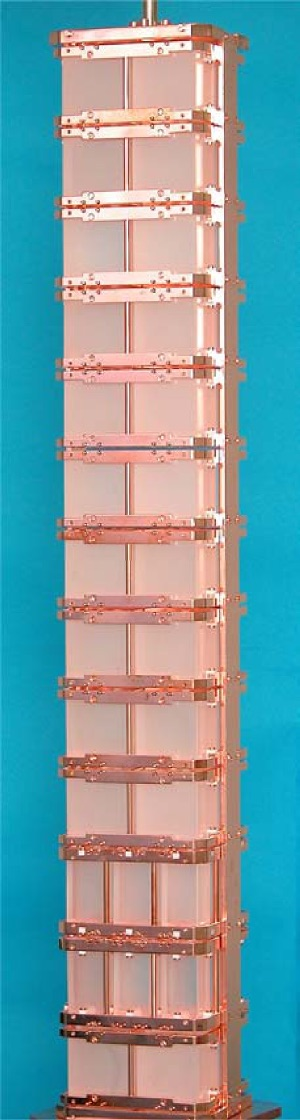
\includegraphics[width=0.8\linewidth, height=0.8\linewidth, keepaspectratio, angle=270, origin = c]{Figures/CUORICINO.jpg}
    \vspace*{-1.5 in}
    \caption[The Cuoricino tower consisting of both big crystals and small unenriched and enriched crystals.]
    {The Cuoricino tower (sideways, with bottom at left) consisting of both big crystals and small unenriched and enriched crystals.}
    \label{fig:Cuoricino_tower}
\end{figure}

With this exposure, Cuoricino determined an experimental limit of $2.8\times10^{25}$ yr (90\% C.L).
During the operation of Cuoricino, a few things were learned that influenced the design choices in CUORE.
As the big crystals with naturally abundant $^{130}$Te had better energy resolution ($6.3 \pm2.5$ keV) than the smaller unenriched ($9.9\pm4.2$ keV) and enriched crystals ($13.9\pm5.3$ keV), the big crystals were selected as the choice for CUORE.
With this resolution for the big crystals, the design goal of the CUORE crystals was set to be 5 keV, and the improved wire bonding method described in \autoref{ssec:Tower Assembly} was developed in order to attain this.
Cuoricino's cryostat was a wet dilution refrigerator that required a liquid helium bath to be refilled every 48 hours, which interrupted data-taking for 3-4 hours at a time.
As this directly affects the detector livetime and stability, CUORE's cryostat is designed as a dry cryostat and makes use of pulse tube cooling at the 4-K stage.
Lastly, as $\alpha$ backgrounds made up a significant portion of the background of Cuoricino in the region of interest, a more rigorous parts selection and cleaning regimen was undertaken for CUORE, which is described in detail in \autoref{ssec:Parts Selection and Cleaning}.

\begin{figure}[htbp]
    \centering
    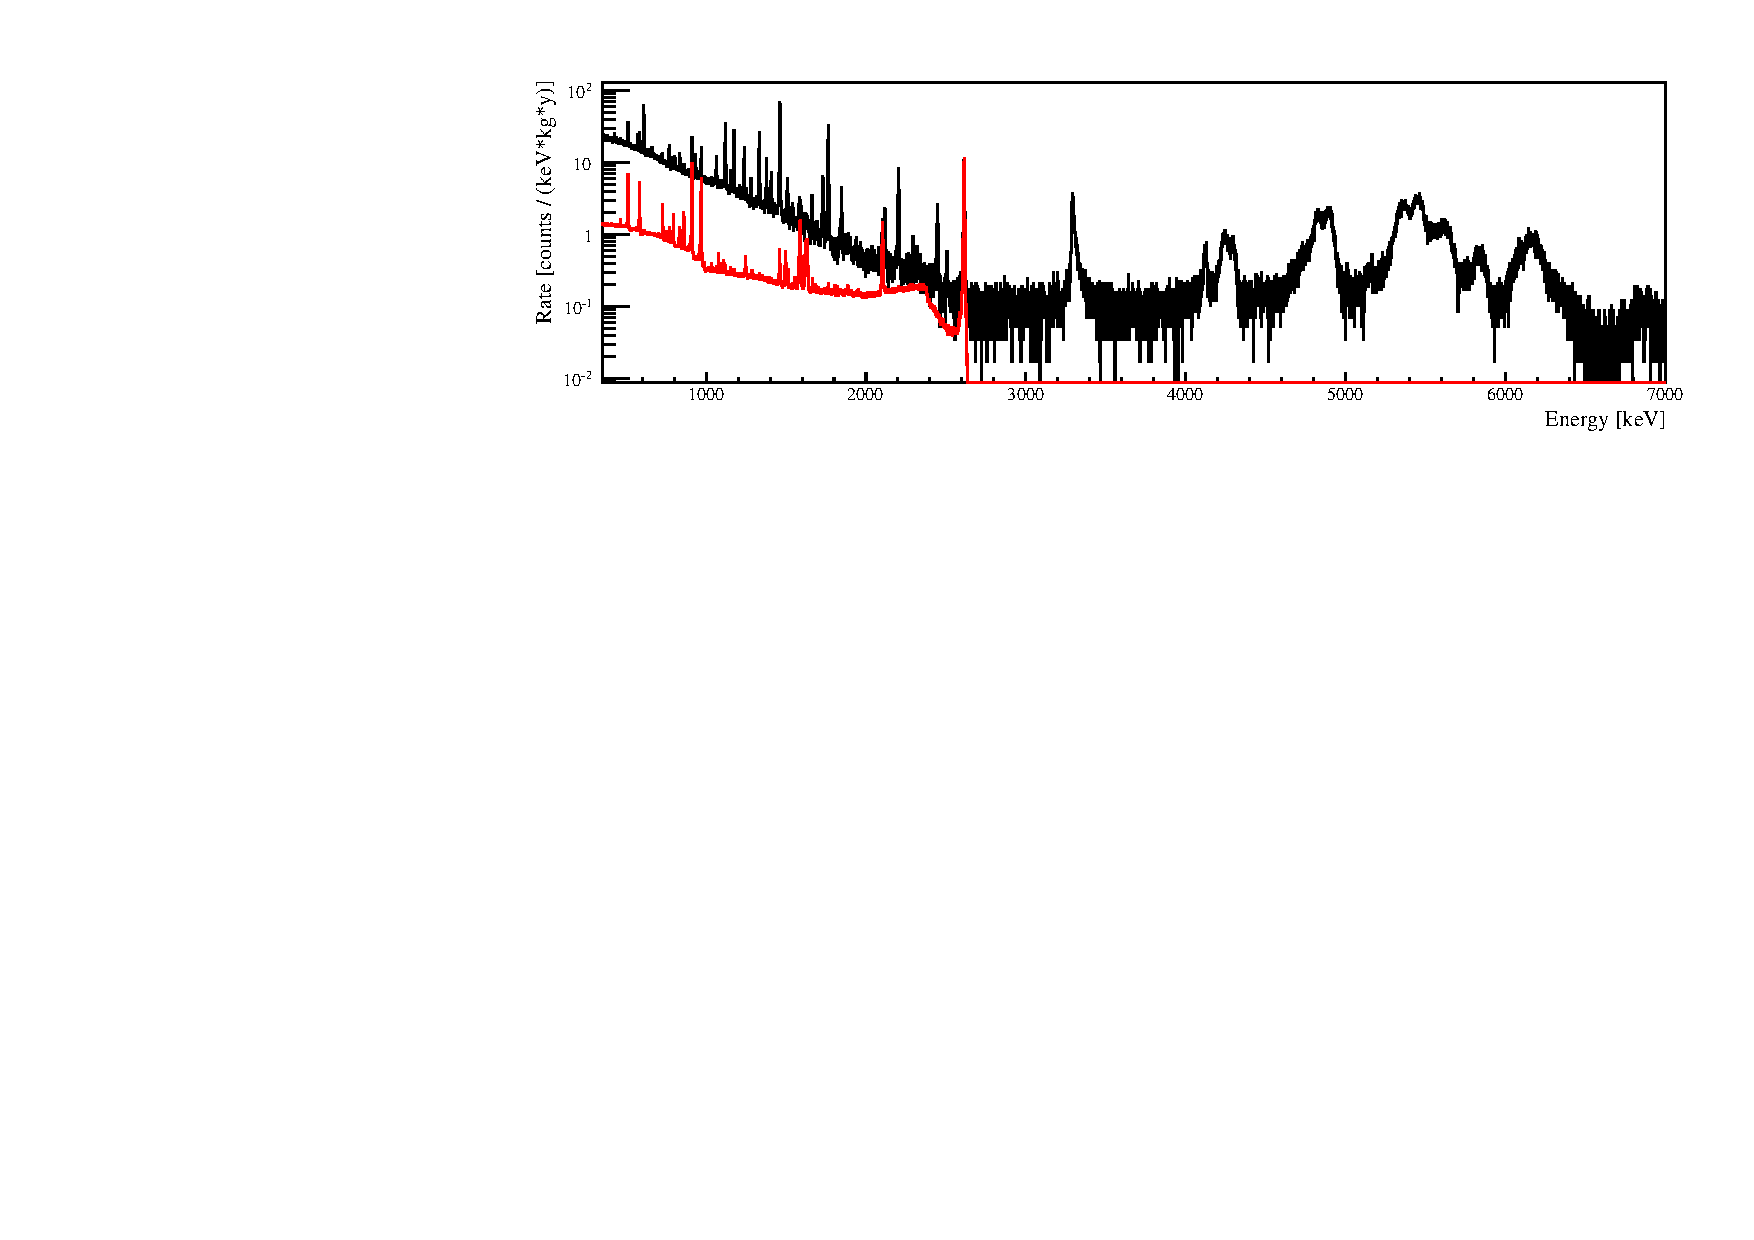
\includegraphics[width=0.8\linewidth]{Figures/CuoricinoSpectrum.pdf}
    \caption[The energy spectrum for Cuoricino in background (black) data along with calibration (red) data which has been normalized to the 2615 keV peak.]
    {The energy spectrum for Cuoricino in background (black) data along with calibration (red) data which has been normalized to the 2615 keV peak.
    The calibration spectrum is normalized to highlight the difference between the background near the 2528 keV Q-value of \zeronubb~due to gammas depositing energy versus that of degraded alphas.}
    \label{fig:cuoricino spectrum}
\end{figure}

\subsection{CUORE-0}
\label{ssec:CUORE-0}

After the completion of the Cuoricino experiment, an intermediate experiment, CUORE-0, was planned while working on completing the CUORE cryostat.
CUORE-0 was meant to bridge the gap between Cuoricino and CUORE by installing a single CUORE-like tower into the Cuoricino cryostat.
In this way, a CUORE-like tower could be studied inside the well-understood Cuoricino cryostat which allowed the changes to the tower to be decoupled from changes to the cryostat.
A schematic of the experimental apparatus can be seen in \autoref{fig:CUORE-0_cryostat_schematic}.

\begin{figure} [htbp]
    \centering
    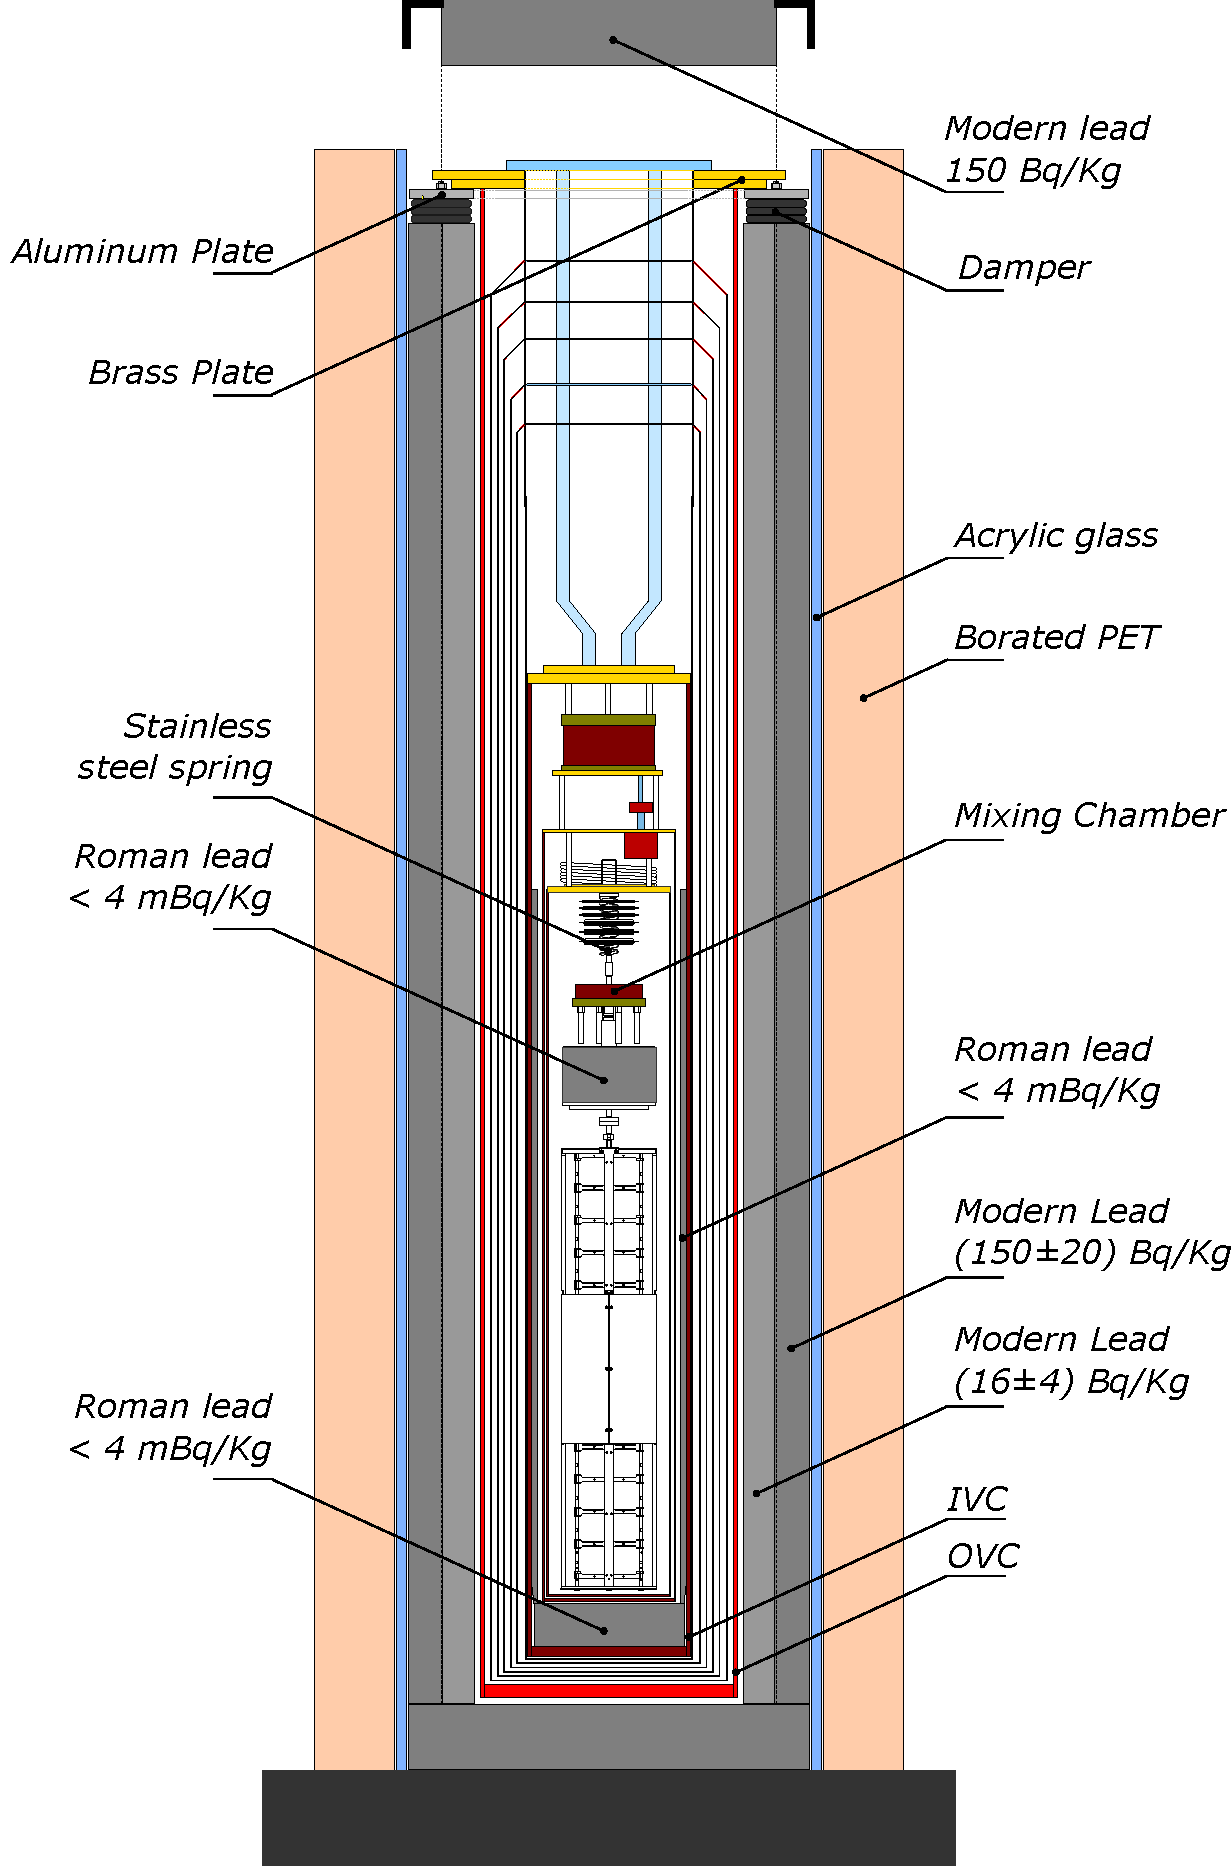
\includegraphics[width=0.8\linewidth]{Figures/CUORE-0_cryostat_schematic.pdf}
    \caption[A schematic of the CUORE-0 experiment.]
    {A schematic of the CUORE-0 experiment in the Cuoricino cryostat (not to scale).
    The CUORE-0 tower is in the center of the cryostat, and the calibration sources are deployed between the OVC and the external lead shield.}
    \label{fig:CUORE-0_cryostat_schematic}
\end{figure}

The purpose of this experiment, besides  making a measurement of \zeronubb, was to validate the improved materials selection and cleaning of the CUORE crystals.
This improvement is quantified in \autoref{fig:cuore-0_vs_cuoricino} where a signficant decease is observed in the \alpha~backgrounds which are due to components nearest to the crystals.
The \gamma~backgrounds are not reduced as significantly as the cryostat is the same between the CUORE and Cuoricino experiments.

\begin{figure}[htpb]
    \centering
    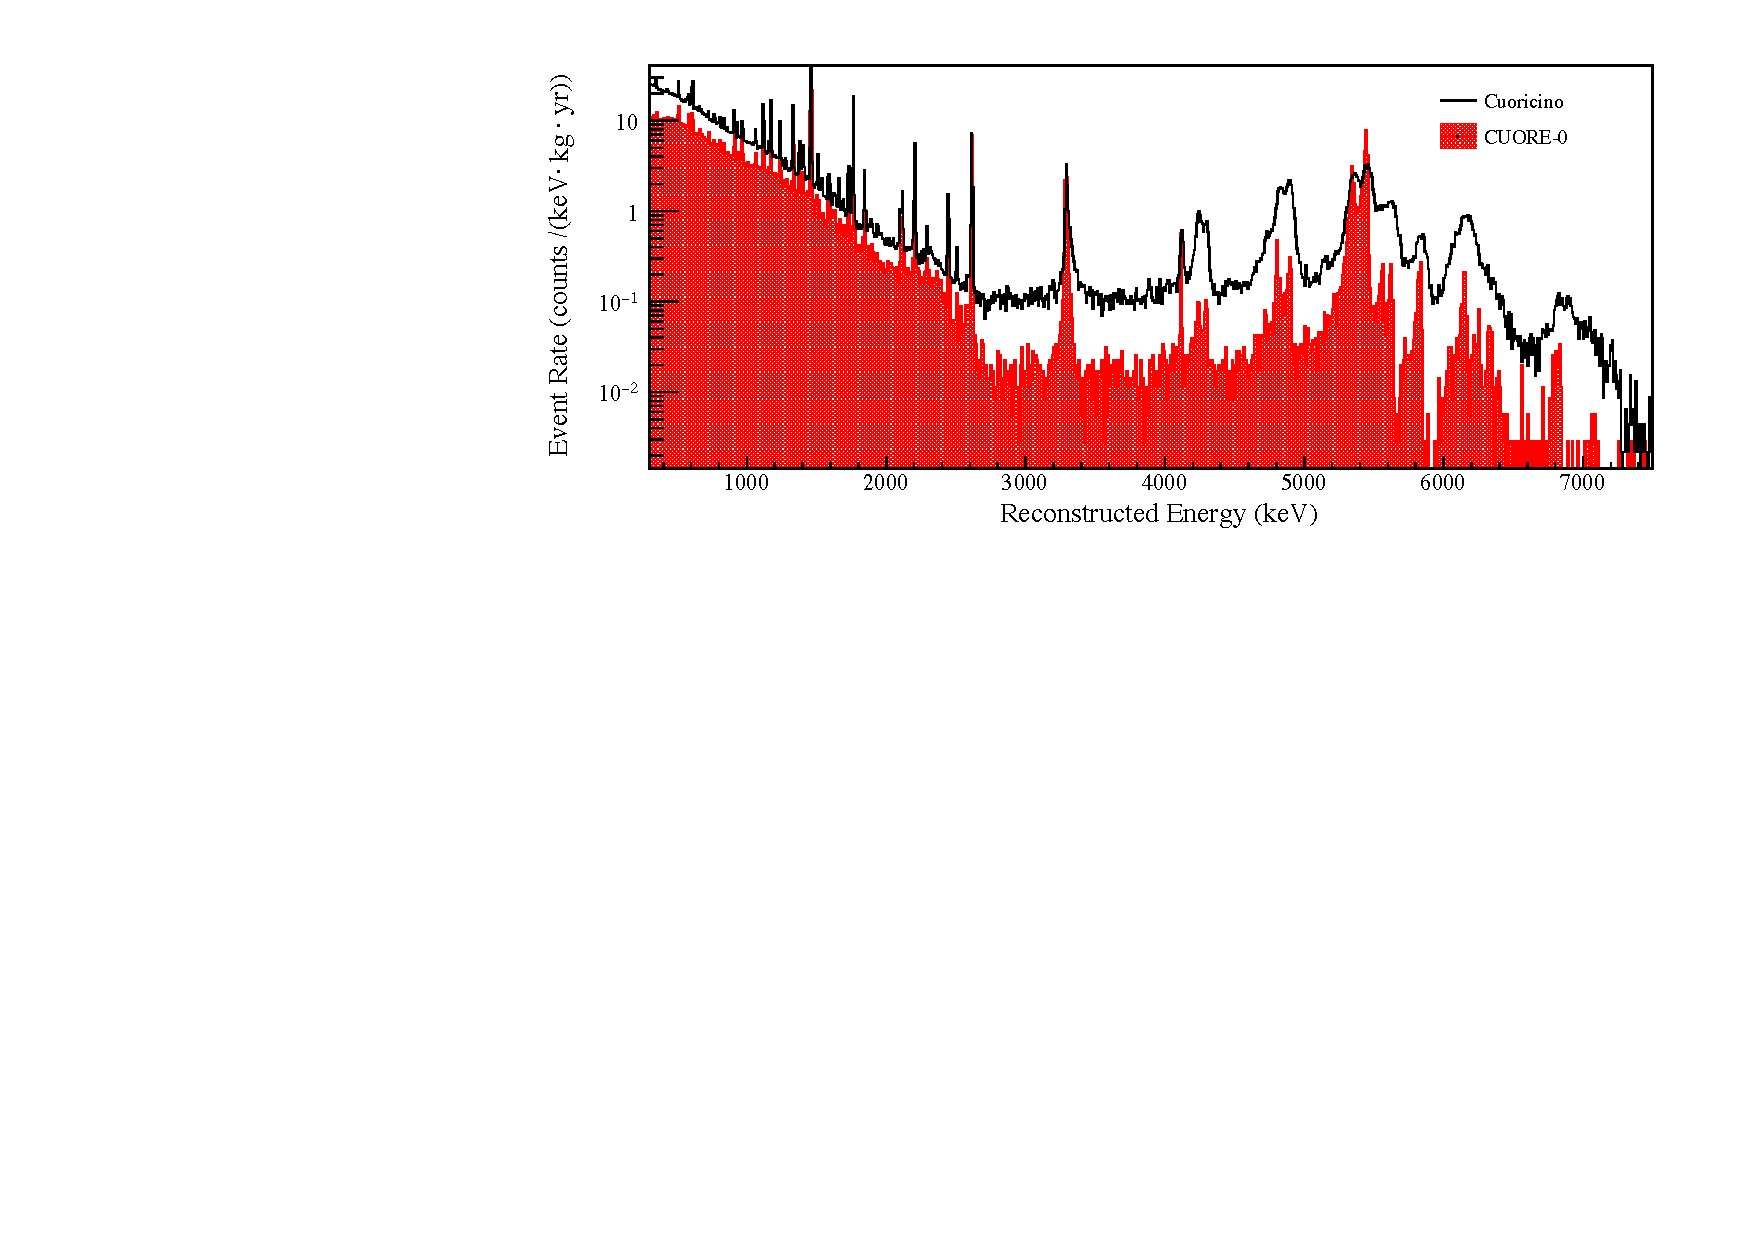
\includegraphics[width=\linewidth]{Figures/CUORE-0_vs_Cuoricino.pdf}
    \caption[A comparison of the backgrounds in the Cuoricino and CUORE-0 exeperiments.]
    {A comparison of the backgrounds in the Cuoricino and CUORE-0 experiments.
    The backgrounds are significantly reduced in the \gamma~ regions as the improved materials selection and cleaning procedures reduced the surface contaminants on the \teotwo~crystals and the copper frames on the tower.
    There is also some improvement on the level of \gamma~ backgrounds, but as the cryostat is the same, those contaminations remain.
    However, one peak in the $\alpha$ region from $^{210}$Po does not decrease, and may be particular to this single tower.}
    \label{fig:cuore-0_vs_cuoricino}
\end{figure}

CUORE-0 collected data between 2013 and 2015, and during this time many analysis and data-collection techniques were refined and improved for use in CUORE.
In particular, from the data collected, CUORE-0 was able to make the most precise measurement of \twonubb~decay in $^{130}$Te at the time, listed in \autoref{tab:2nuHalfLife} \cite{Alduino:2016vtd}.
In addition, CUORE-0 also performed a search for \zeronubb~and, in a combined analysis with the Cuoricino experiment, formed the most stringent limit at the time for \zeronubb~decay in $^{130}$Te with a limit of $T^{0ν}_{1/2}>4.0\times10^{24}$ yr \cite{Alfonso:2015wka}.

\section{CUORE Cryostat}
\label{sec:CUORE Cryostat}

Since the heat capacity of the CUORE crystals is so strongly dependent on temperature, it is critically important to have a system that can cool down the crystals to a base temperature of $\sim10$ mK and operate in a stable condition over long periods, up to CUORE's 5-year planned livetime.
To this end, a cryogen-free custom cryostat was constructed to house the crystals, shown in \autoref{fig:cryostat_cad_cutout} \cite{cryostat_commissioning}.
The cooling components of the cryostat are pulse tubes that cool the cryostat stages at 40-K\footnote{Naming convention: I use ``40-K" to denote cryostat stages and ``40 K" to denote temperatures.} and 4-K and a dilution refrigerator that is responsible for maintaining the coldest regions of the cryostat, including the crystals inside the 10-mK stage.
In addition to cooling the crystals, the cryostat also houses the shielding for the crystals such as the internal and, since this is a low-background experiment, is made of radiopure materials, especially near the detectors themselves.
Due to the background requirements and because the crystals themselves are housed inside the 10-mK shield, the cryostat was assembled underground at LNGS inside of a clean room.
Inside the cryostat, there are two vacuum volumes, the Outer Vacuum Chamber (OVC) and the Inner Vacuum Chamber (IVC).
The OVC consists of all the volumes outside of the 4-K stage, and is isolated from the IVC, which consists of all the volumes inside the 4-K stage, including the detectors.

\begin{figure}[htbp]
\centering
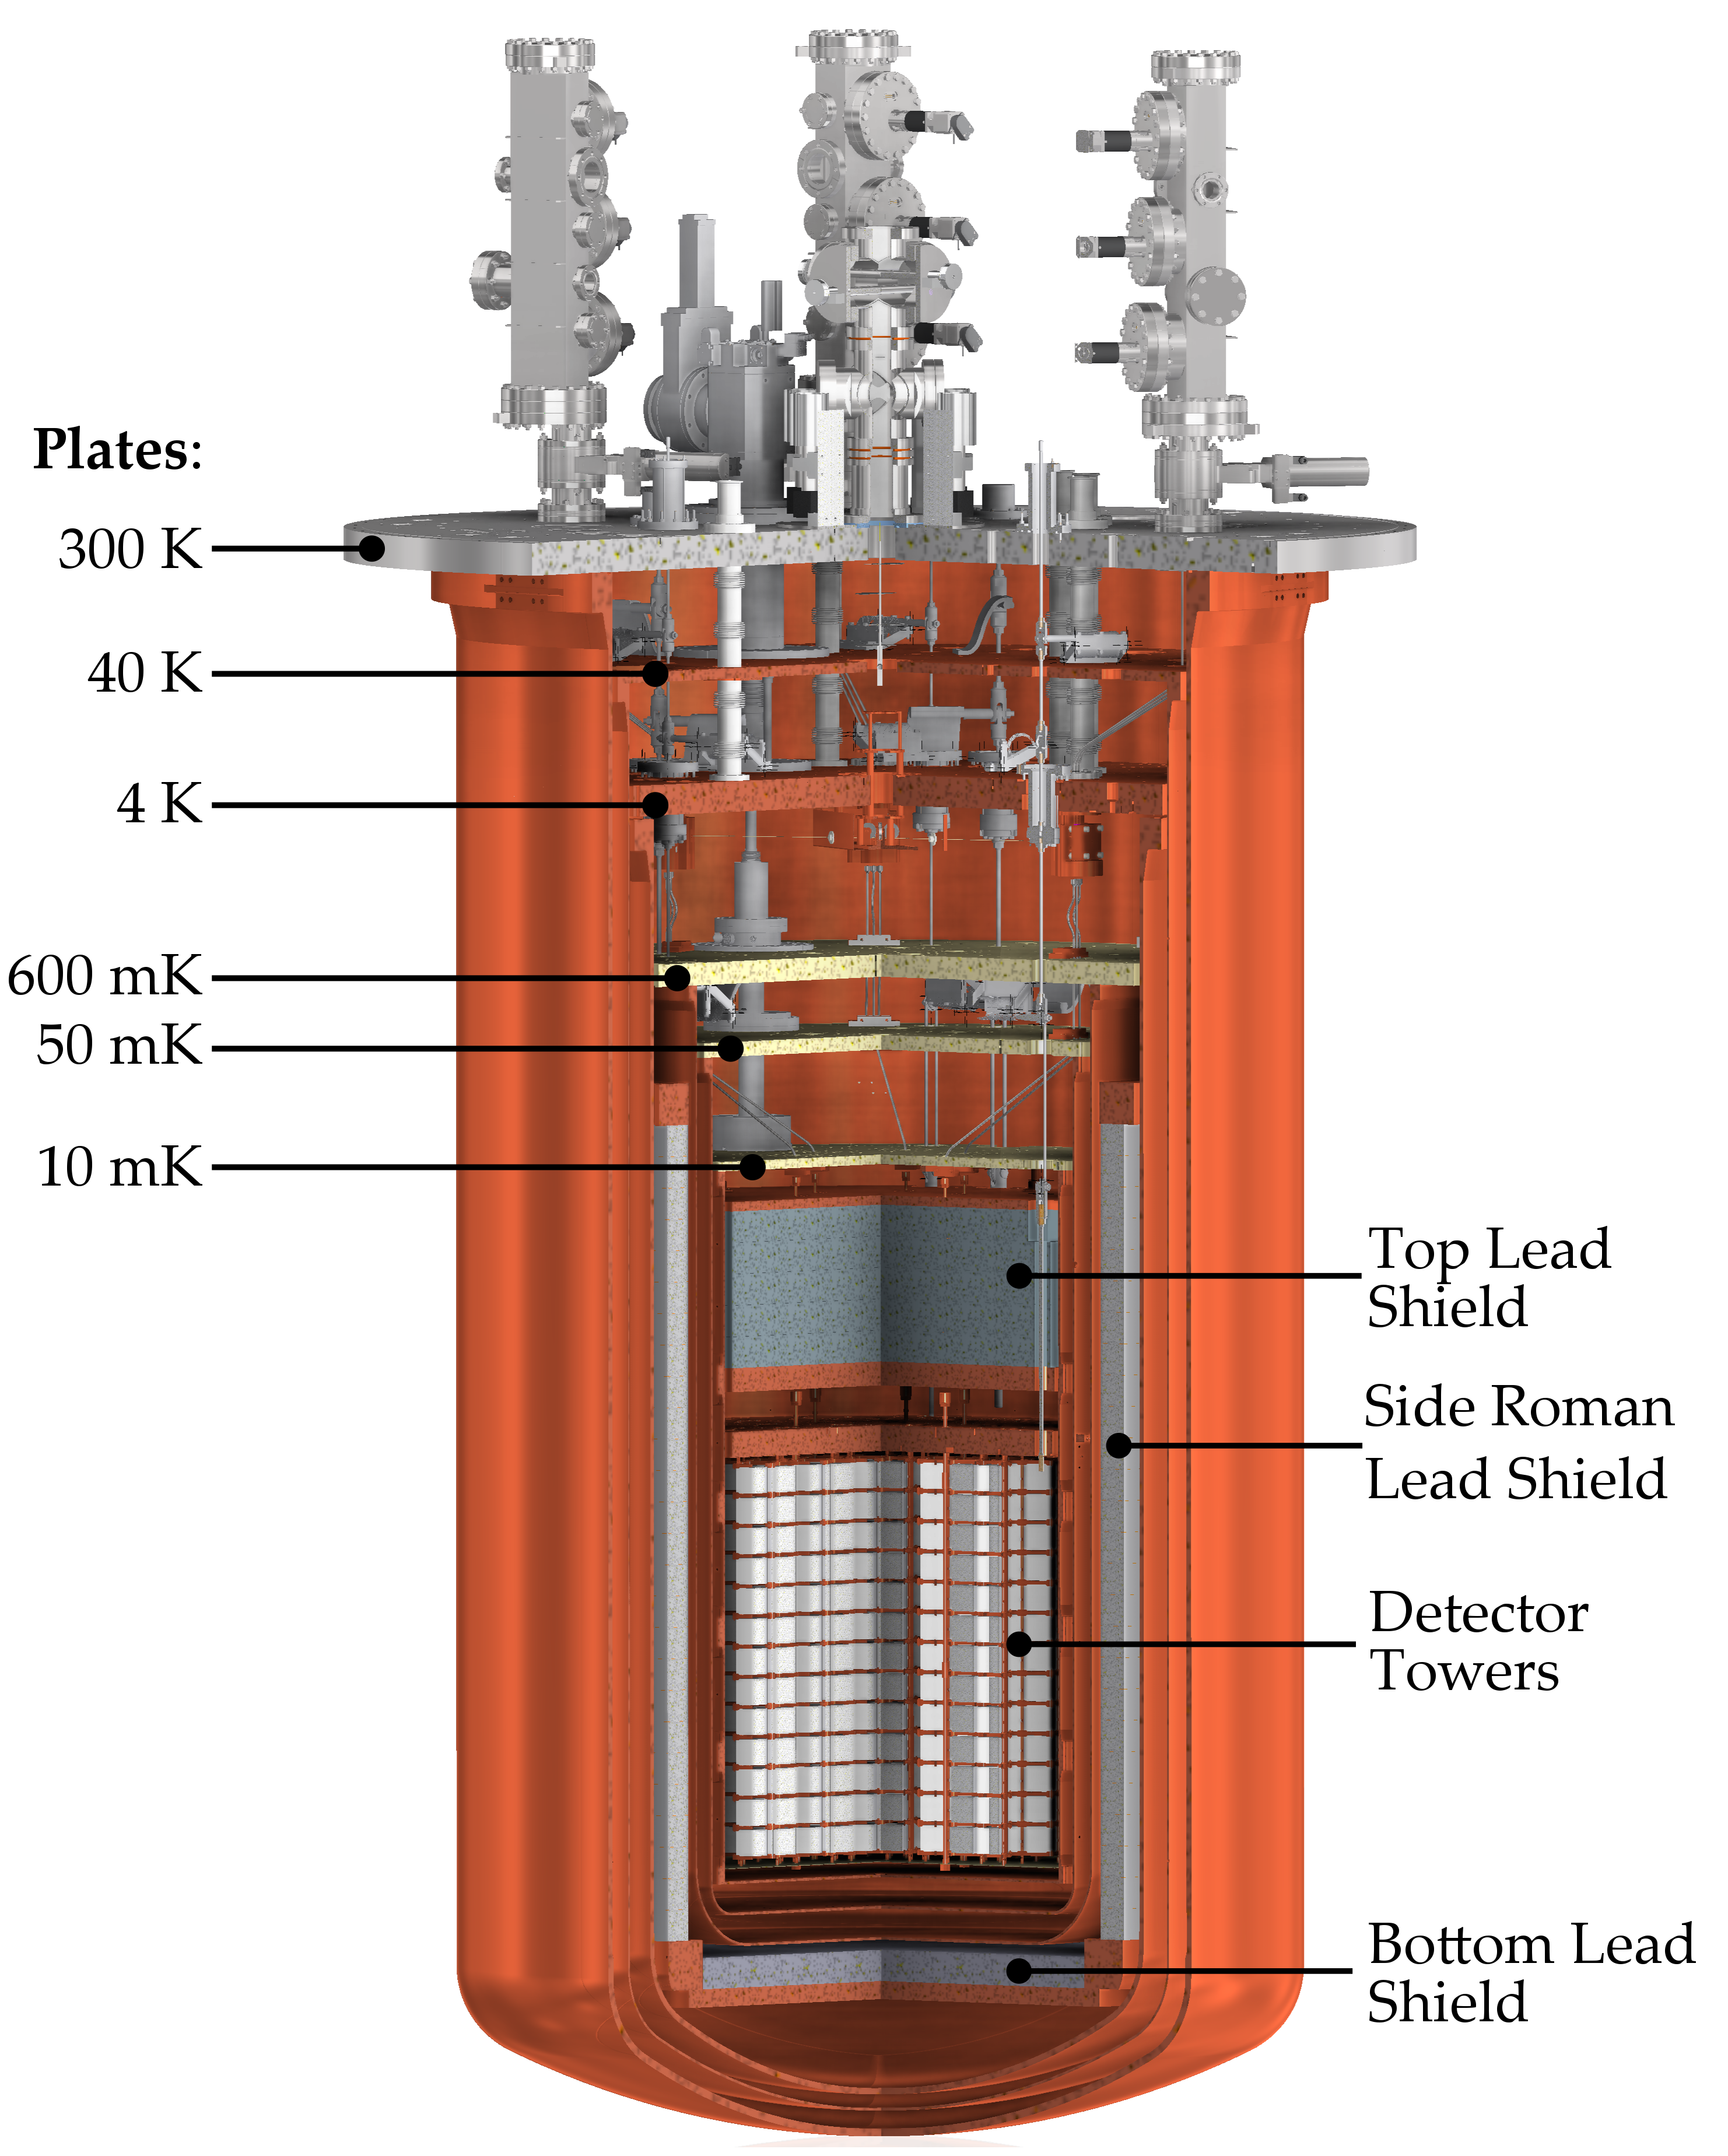
\includegraphics[width=\linewidth]{Figures/cryostat_Adjusted.png}
\caption[CAD cutaway of the CUORE cryostat.]
{A CAD drawing of a cutaway the CUORE cryostat showing the internal shielding of the cryostat.
The temperature stages of the cryostat are also shown.
Not included are the external shields which extend around the sides of the cryostat, shown in \autoref{fig:external_shielding}.
Figure courtesy of the CUORE collaboration.}
\label{fig:cryostat_cad_cutout}
\end{figure}

\subsubsection*{Detector Shielding and Vibration Isolation}
As noted above, the detectors need to be shielded from the environment and even from radioactivity in the shielding itself.
Starting from the outside of the experiment, shown in \autoref{fig:external_shielding}, there is an external lead shield with a layer of polyethylene and boric acid that surrounds the cryostat.
This $\sim70$ ton, 25 cm thick lead shielding acts to shield from the environmental gammas from LNGS, and the 18 cm thick polyethlene and 2 cm thick boric acid (H$_3$BO$_3$ powder) thermalize and absorb environmental neutrons.
This external shielding can be raised and lowered as needed, and remains lowered while working on the cryostat, and raised during physics data-taking.
Inside this external shielding is the cryostat, suspended from the main support plate above by three steel ropes.
This plate is supported by sand-filled columns, resting on rubber dampeners which act to seismically isolate the main support plate, and thus the cryostat) from the ground.
This is a particularly important component given the seismic nature of the area around LNGS as vibrations contribute to low-frequency noise in CUORE, as, at the low temperatures of CUORE, the frictive heating from motion of the cryostat affects the sensitivity of the CUORE bolometers.
In fact, even despite all these components, we set bad intervals, \color{red} discussed later in subsubsection bad intervals \color{black} during particularly intense seismic events around the globe.
At the top of the cryostat, the 300-K plate supports the 40-K, 4-K, and 600-mK plates by segmented steel rods.
Each of these plates also holds a corresponding cylindrical vessel that surrounds the inner vessels.
In addition, these vessels act as a radiation shield, both for thermal and particle radiation \color{red} better wording here? \color{black}.
In order to minimize the radioactivity of these components, with over 7 tonnes of mass, these plates and vessels are made of Oxygen-Free Electronic (OFE) copper (99.99\% Cu), with the exception of the 300-K plate and the top of the 300-K vessel which is made of the stronger austenitic stainless steel due to the load it carries. This radioactivity constraint carries over to the superinsulation used to cover the 40-K and 4-K stages of the cryostat, which is needed to reduce the thermal radiation heat load on the vessels, and was optimized for a choice of 17 kg in 30 and 10 layers of aluminized mylar and polyester foil for the 40-K and 4-K stages, respectively.

\begin{figure}
    \centering
    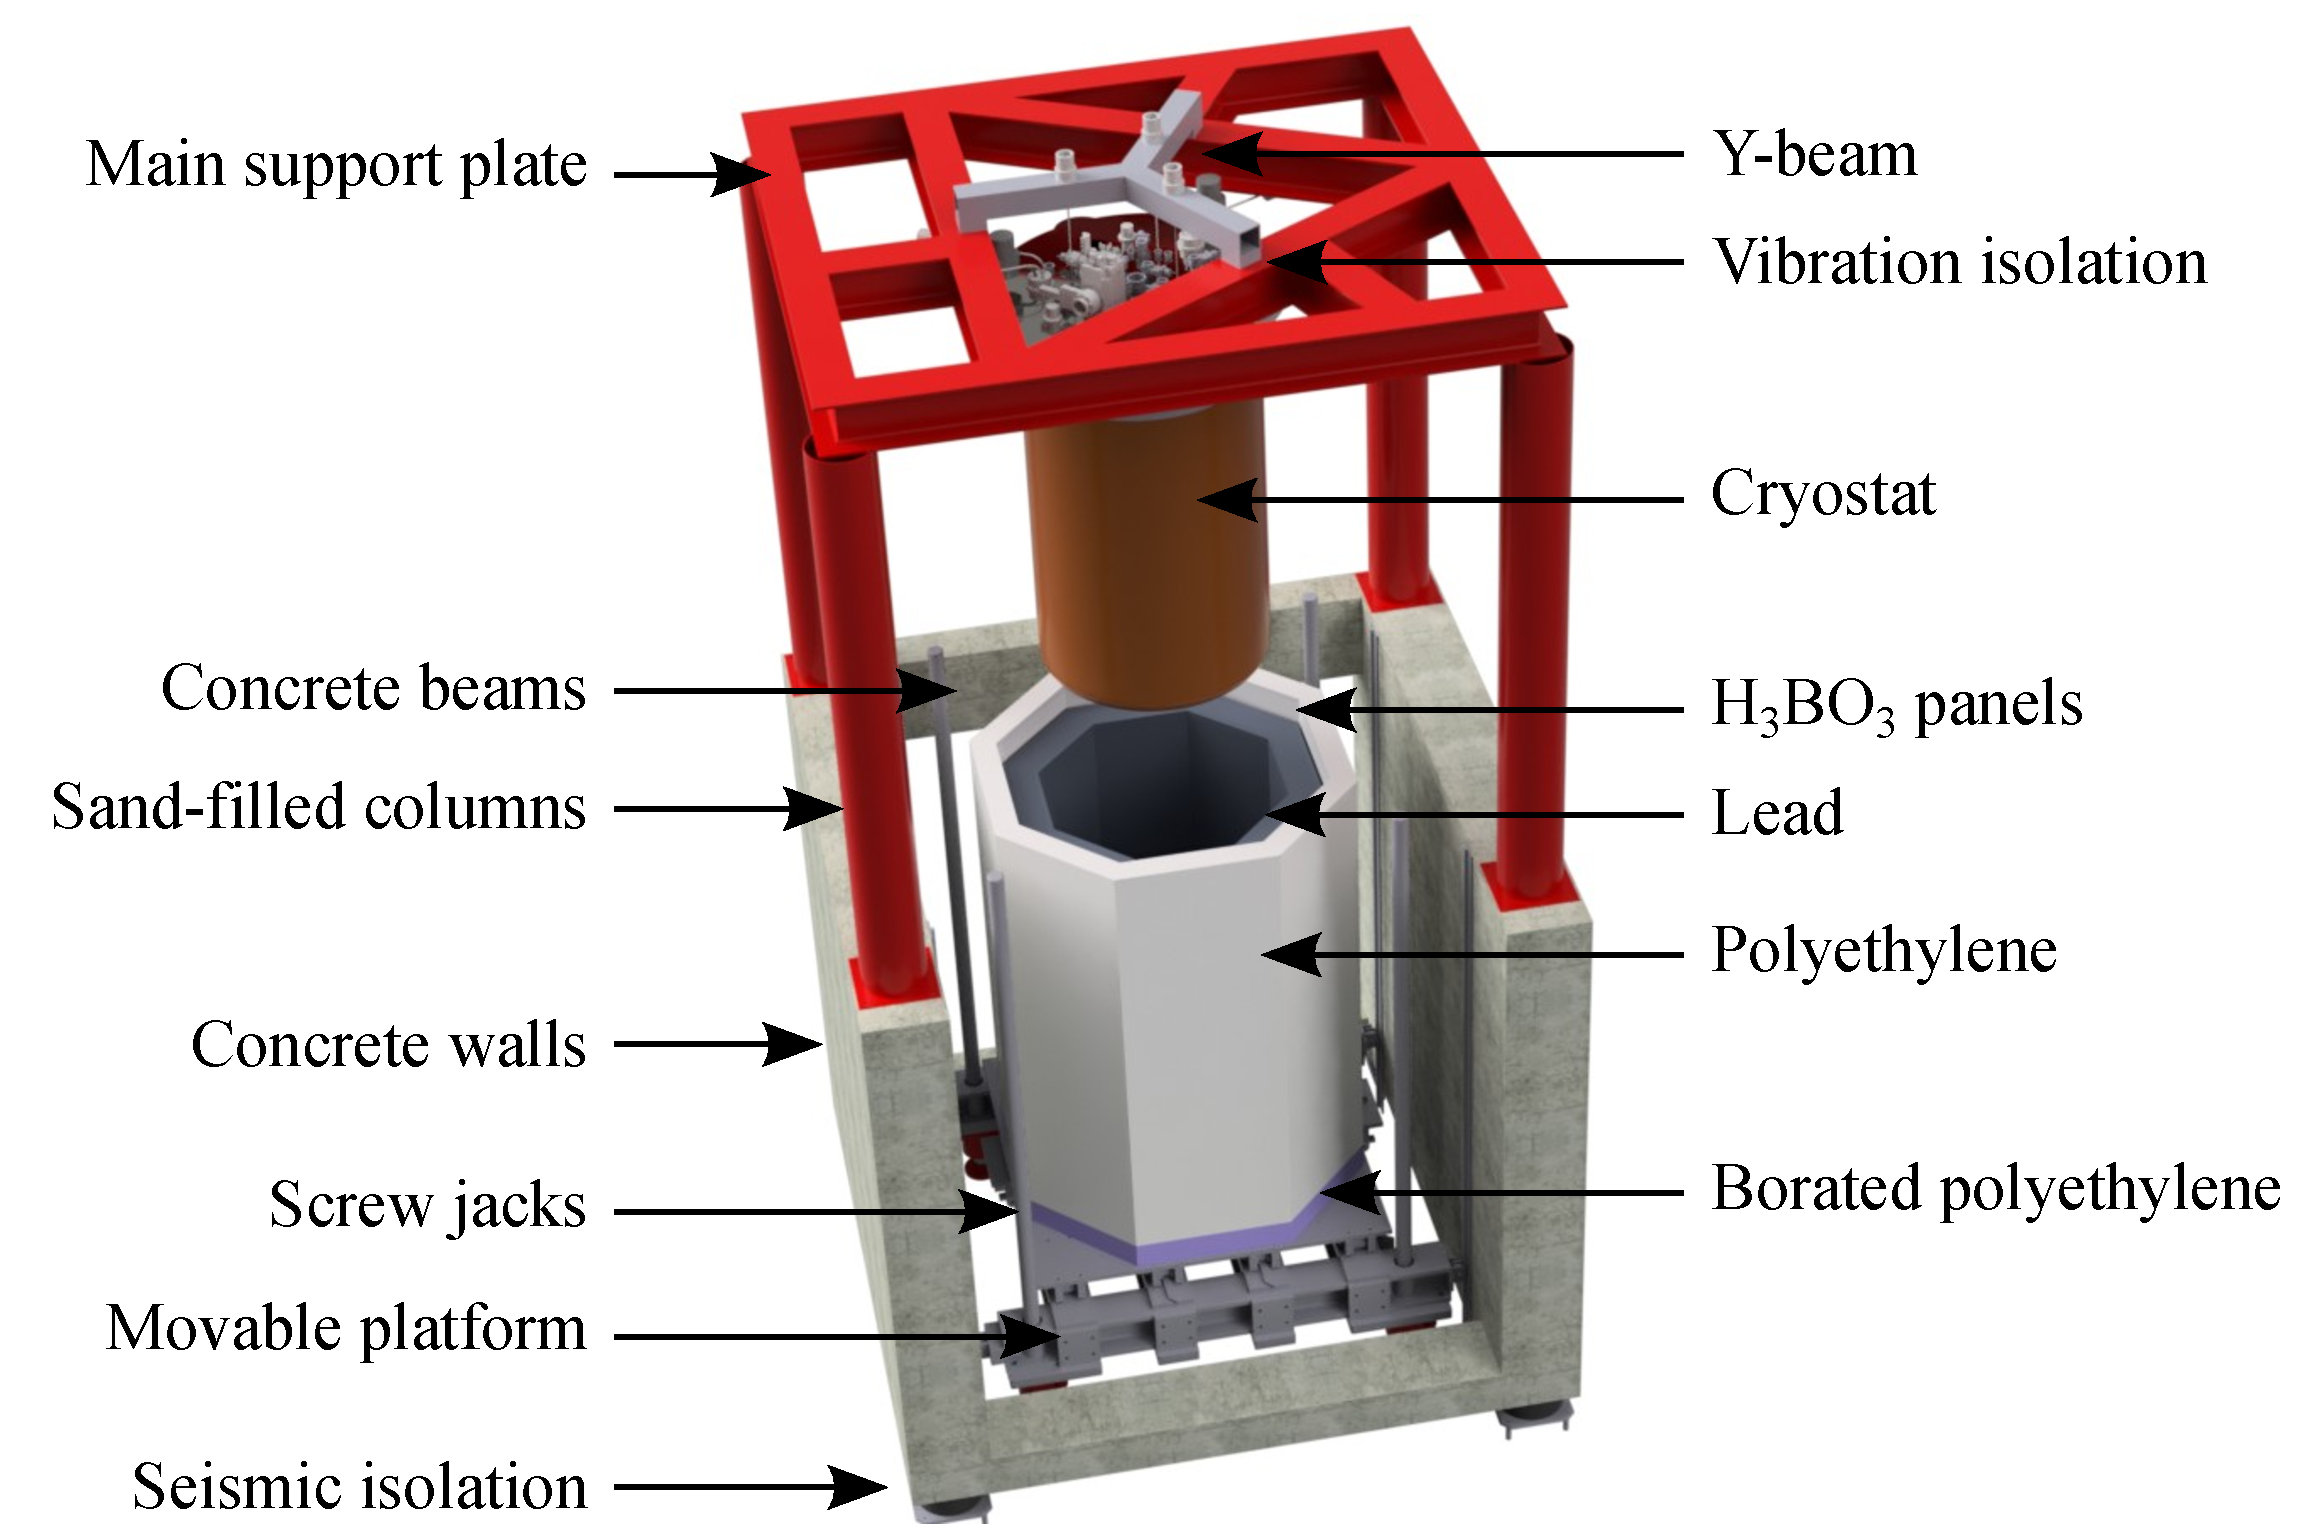
\includegraphics[width=\linewidth]{Figures/Hut_ShieldingDown_02.pdf}
    \caption[The external shielding and supports of the CUORE cryostat.]
    {The external shielding and supports of the CUORE cryostat.
    The external lead shields, with polyethylene and borated polyethlyene, is shown lowered down below the cryostat and is raised up around the cryostat during operation.
    The crystat is suspended above, and the support structure is designed to minimize the mechanical coupling of the cryostat to the outside world and the resultant vibrational noise.}
    \label{fig:external_shielding}
\end{figure}
Inside the 4-K stage of the cryostat, additional 6 cm thick lead shielding is used to further reduce radioactive backgrounds. This shielding comprises over 4 tonnes of ancient shipwrecked lead \cite{roman_lead} and covers the sides and bottom of the cryostat.
As lead when extracted from the ground contains $^{210}$Pb from the $^{238}U$ decay chain with a half-life of 22 years, we use this lead that was shipwrecked between 80 and 50 B.C.E. to line this inner shield of our detectors, shown in \autoref{fig:roman_lead_shield}.
This lead has a contamination of $^{210}$Po less than 10 mBq/kg\footnote{$^{210}$Po in modern lead can reach values of 2500 Bq/kg.} and is thus more suitable for use in the most sensitive regions of our cryostat \cite{ALESSANDRELLO1998163}.  
\begin{figure}
    \centering
    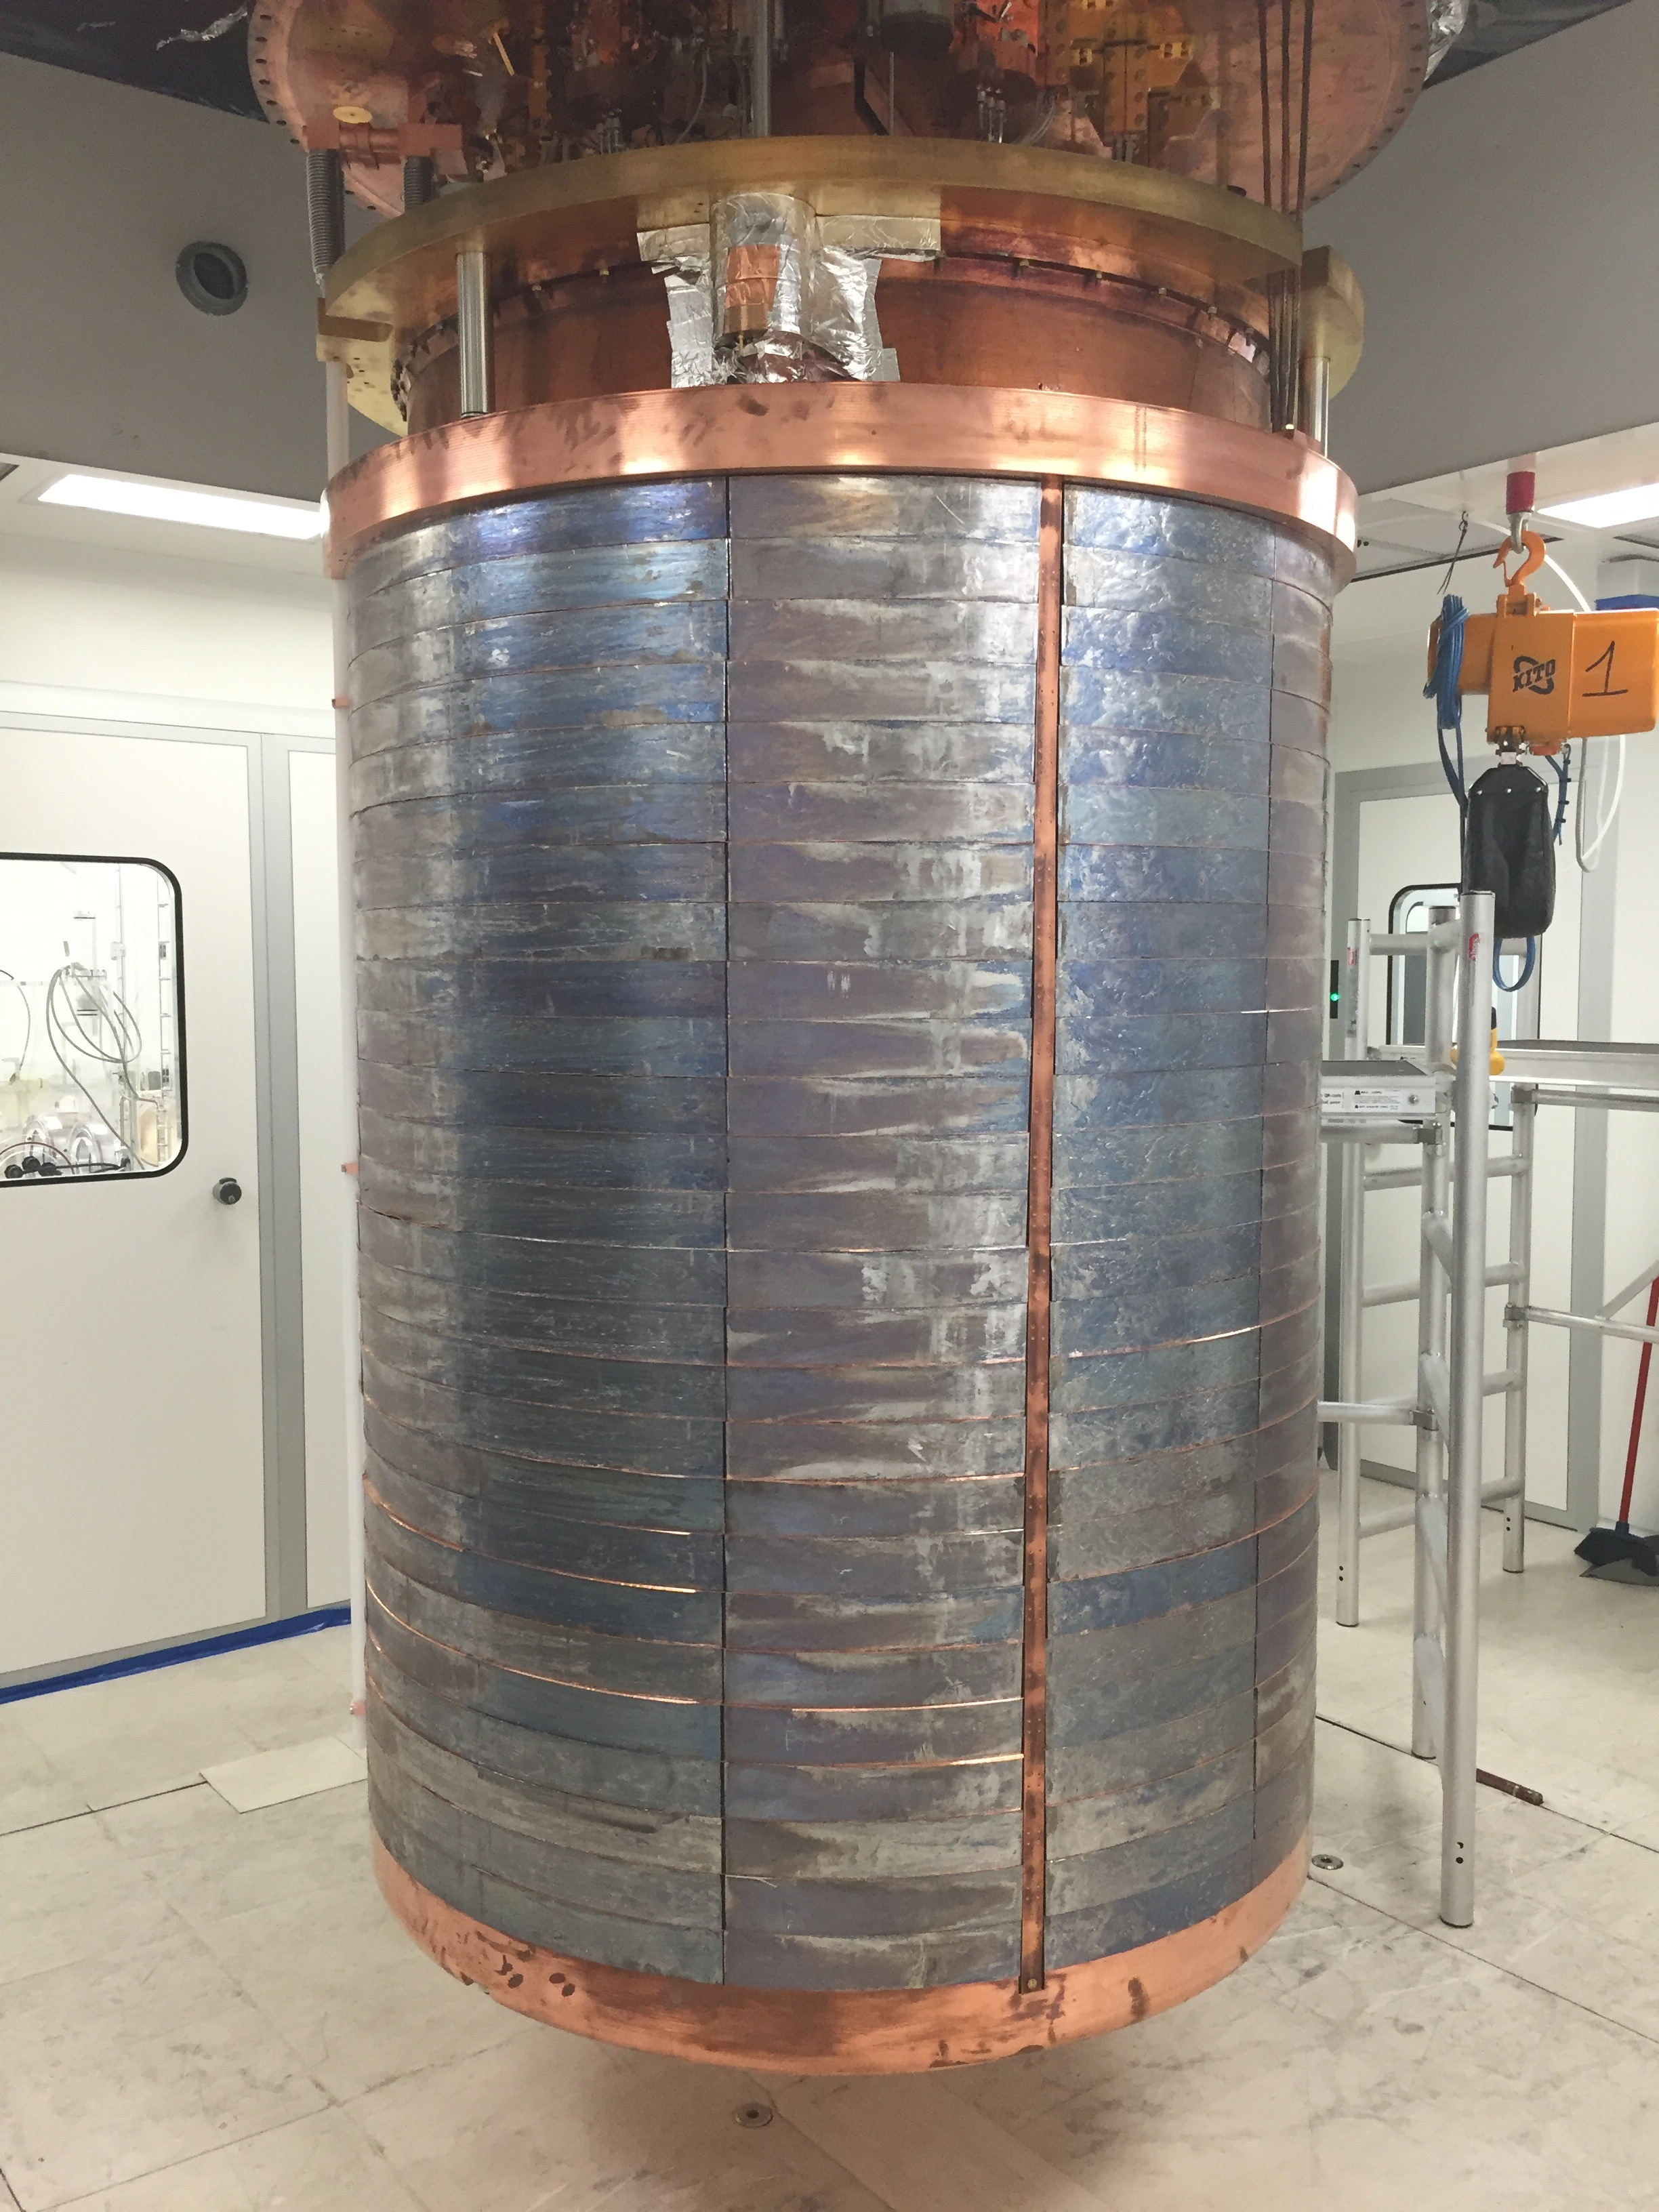
\includegraphics[width=0.4\linewidth, height=0.4\pageheight, keepaspectratio]{Figures/roman_lead_shield.jpg}
    \caption[The roman lead shield installed inside the 4-K vessel.]
    {The roman lead shield installed inside the 4-K vessel. The shield extends laterally around the detector region and a separate piece is below (not visible).}
    \label{fig:roman_lead_shield}
\end{figure}
The 600-mK plate holds the 50-mK plate, which in turn holds up the 10-mK plate, with a double Kevlar rope and a copper rod, respectively.
This rope is used to minimize the heat load at these coldest stages with the least cooling power, see \autoref{tab:cryostat_cooling_power}, and the copper rod is used due to background constraints near the detector region.
Below the 10-mK plate but thermally connected with the 50-mK stage, there is an additional lead shield, consisting of 2 tonnes of modern lead in five 6 cm disks between two copper plates, above the detectors.
This is the final main shield for gammas produced in components of the cryostat, although the copper plate that holds the crystals, called the tower support plate (TSP) also shields the detectors which are mounted to the bottom of the plate.
The TSP hangs separately from the rest of the cryostat and is suspended from the steel Y-beam on three Minus K\footnote{\RaggedRight\url{https://www.minusk.com/}} vibration isolators on the MSP.
Part of the suspension is Kevlar rope that connects the TSP to the copper and steel suspension rods above, which, in addition to reducing the thermal load of the detector array, also serves to protect the crystals in case of a seismic event. 
This assembly acts to cause the detectors to essentially hang freely and avoids pendulum-like low frequency oscillations of the tower array which would cause frictive heating.
While the 50-mK plate and vessel are composed of OFC copper like the warmer stages, the 10-mK plate and vessel, the copper holding the top lead, and the TSP are all comprised of NOSV copper due to the strict background requirements of parts in the detector region.
In addition, the side of the 10-mK plate facing the detector is covered by thin NOSV copper tiles that had been cleaned with the same procedure as for copper in the tower frames.
    
\subsubsection*{Cryostat Cooling Systems}
\label{sssec:Cooling Systems}
Not only does the cryostat shield the detectors from radiation, but it also needs to cool the detectors to temperatures of $\sim$10 mK.
Therefore, a dilution refrigerator is used as the main cooling mechanism of the cryostat.
A dilution refrigerator works by taking advantage of the phase boundary between dilute and concentrated phases of a $^3$He and $^4$He mixture, shown in \autoref{fig:He_phase_diagram}.
In the mixing chamber of the dilution refrigerator on the 10~mK stage of the CUORE cryostat, $^3$He flows from the concentrated phase to the dilute phase.
This process extracts energy from the environment of the mixing chamber, and, by extension, the coldest stages of the cryostat, as energy is required to move the $^3$He across the phase boundary\footnote{Of course, the Universe's entropy is not reduced by this exchange and additional energy is used to induce this endothermic cooling.}.
As noted in \autoref{ssec:CUORE-0}, one of the main cryostat changes between the previous experiments of CUORE-0 and CUORE was the change to a cryogen-free cryostat that uses pulse tubes instead of an external supply of liquid nitrogen, helium, and a 1~K bath.
This change allows for increased livetime of the experiment as data-taking does not need to be interrupted by the need to refill the bath, especially as this would become even more disruptive given the tonnes of material that would need to be cooled.
However, this does come at a cost of increased mechanical noise as the five pulse tubes in CUORE input mechanical vibrations onto the cryostat.
Worsening this issue, the five pulse tubes\footnote{PT415-RM from Cryomech \url{https://www.cryomech.com/products/pt415/}} on CUORE are not symmetrically aligned due to space constraints, and it is nontrivial to find a phase configuration that minimizes the noise, requiring an in-depth scan of varying pulse tube phases to determine when the mechanical noise induced by the pulse tubes is minimized over the detectors.

\begin{figure}[htbp]
    \centering
    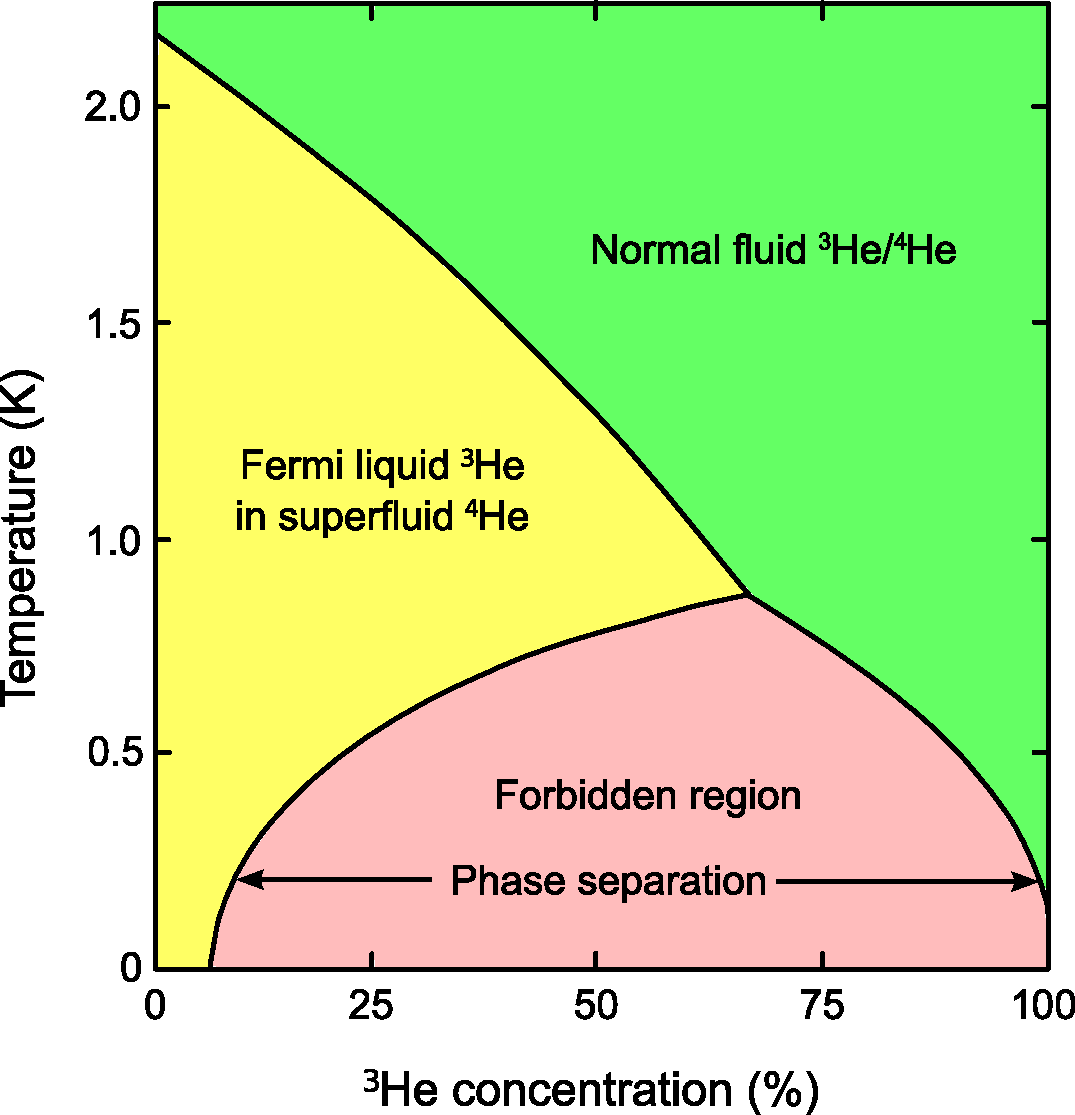
\includegraphics[width=0.6\linewidth]{Figures/Helium_phase_diagram.pdf}
    \caption[Phase diagram for $^{3}$He and superfluid $^{4}$He.]
    {Phase diagram for $^{3}$He and superfluid $^{4}$He.
    The separation between the dilute and concentrated phases provides the power that cools the cryostat down to mK-scale temperatures.}
    \label{fig:He_phase_diagram}
\end{figure}

Inside the cryostat, the components necessary for the operation of the dilution refrigerator are the mixing chamber on the 10-mK plate, the heat exchanger on the 50-mK plate, and the still on the 600-mK plate.
Outside the cryostat, the pulse tubes are responsible for pumping the $^3$He out of the still and back down into the mixing chamber.

In addition to the dilution refrigerator and pulse tubes, an additional system called the Fast Cooling System is also used to cool down the CUORE cryostat from room temperature.
This system is needed since pulse tubes are not designed for sustained operations at warm temperatures and the tonnes of material that is needed to be cooled down.
With the Fast Cooling System, a helium exchange gas is pumped into the IVC at a pressure of $\sim1$bar, which cools the cryostat down to 200 K.
Once this occurs, the pulse tubes are turned on, and later, once the cryostat reaches 50 K, the Fast Cooling System is turned off and and nearly all of the exchange gas is removed, with only a few mbar left to assist with the cooldown of the coldest stages down to 10 K.
The cooldown is finally completed by the DU, which cools the detectors down to 10 mK.
With these systems, the cooldown of the CUORE cryostat can be effected in $\sim20$ days.

\begin{table}[htbp]
    \centering
    \begin{tabular}{c|c}
    \hline
    \hline
    Thermal Stage     & Cooling Power \\
    \hline
    40-K     & 40~W \\
    4-K      & 1.5~W \\
    Dilution unit*    & 10~$\mu$W at 12~mK \\
    \hline
    \hline
    \end{tabular}
    \caption[The cooling power of the cryostat at varying thermal stages.]
    {The cooling power of the cryostat at varying thermal stages.
    The power is maximized in warmer stages, but decreases significantly towards the coldest stages.
    Note: the thermal power of the dilution unit was determined in a test cryostat, but should be consistent with the cooling power in CUORE*.}
    \label{tab:cryostat_cooling_power}
\end{table}
\subsubsection*{Cryostat Radiopurity}
As mentioned above, the cryostat also needs to both shield the detectors from outside radioactive sources and simultaneously not contribute to the radioactive backgrounds in the detectors.
It is for this reason, for example that high-purity NOSV copper is chosen for the cryostat components closest to the detectors and that the 4.5 tons of side and bottom lead shielding was chosen to be low-radioactivity ancient Roman lead.
In addition, in order to minimize the effect of cosmogenic activation on the background, the entire CUORE cryostat was assembled and stored underground, although the process of machining and cleaning the components needed to be undertaken aboveground.
The background contamination of these ``far" components, as opposed to the ``near" components in \autoref{tab:NearDetectorSources_Bulk}, is shown in \autoref{tab:FarDetectorSources_Bulk}. 

\begin{table}[htbp]
\centering
\caption[90\% upper limits of $^{232}$Th and $^{238}$U bulk contamination of sources in the cryostat and external shielding.]
{90\% upper limits of $^{232}$Th and $^{238}$U bulk contamination of sources in the cryostat and external shielding.
Table from \cite{Alduino:2017qet}.}
\label{tab:FarDetectorSources_Bulk}
\begin{tabular}{lll}
\hline
\hline
Material         & $^{232}$Th [Bq/kg]         & $^{238}$U [Bq/kg]    \\
\hline
Cu OFE             & $<6.4\times10^{-5}$ & $<5.4\times10^{-4}$      \\
Roman Pb            & $<4.5\times10^{-5}$ & $<4.6\times10^{-5}$      \\
Modern Pb            & $<1.4\times10^{-4}$ & $<1.4\times10^{-4}$      \\
Super-insulation  & $(11\pm2)\times10^{-3}$ & $<2.4\times10^{-3}$      \\
Rods  & $(4\pm2)\times10^{-4}$ & $(8\pm2)\times10^{-4}$      \\
300-K Plate & $(4.5\pm0.5)\times10^{-3}$ & $(1.6\pm0.5)\times10^{-3}$      \\
\hline
\hline
\end{tabular}
\end{table}

As shown in \autoref{eq:sensitivity_short}, the sensitivity of CUORE to \zeronubb~depends on the inverse square root of the background near the decay Q-value.
As such, the background goal of CUORE is to have no greater than 0.01 counts/keV/kg/yr in the region of interest (ROI) defined to be a 100 keV interval from 2470 keV to 2570 keV.
The simulated effect of all the sources, including from cryostat components and shielding, is shown in \autoref{fig:cuore_background_budget}.

\begin{figure}[htbp]
\centering
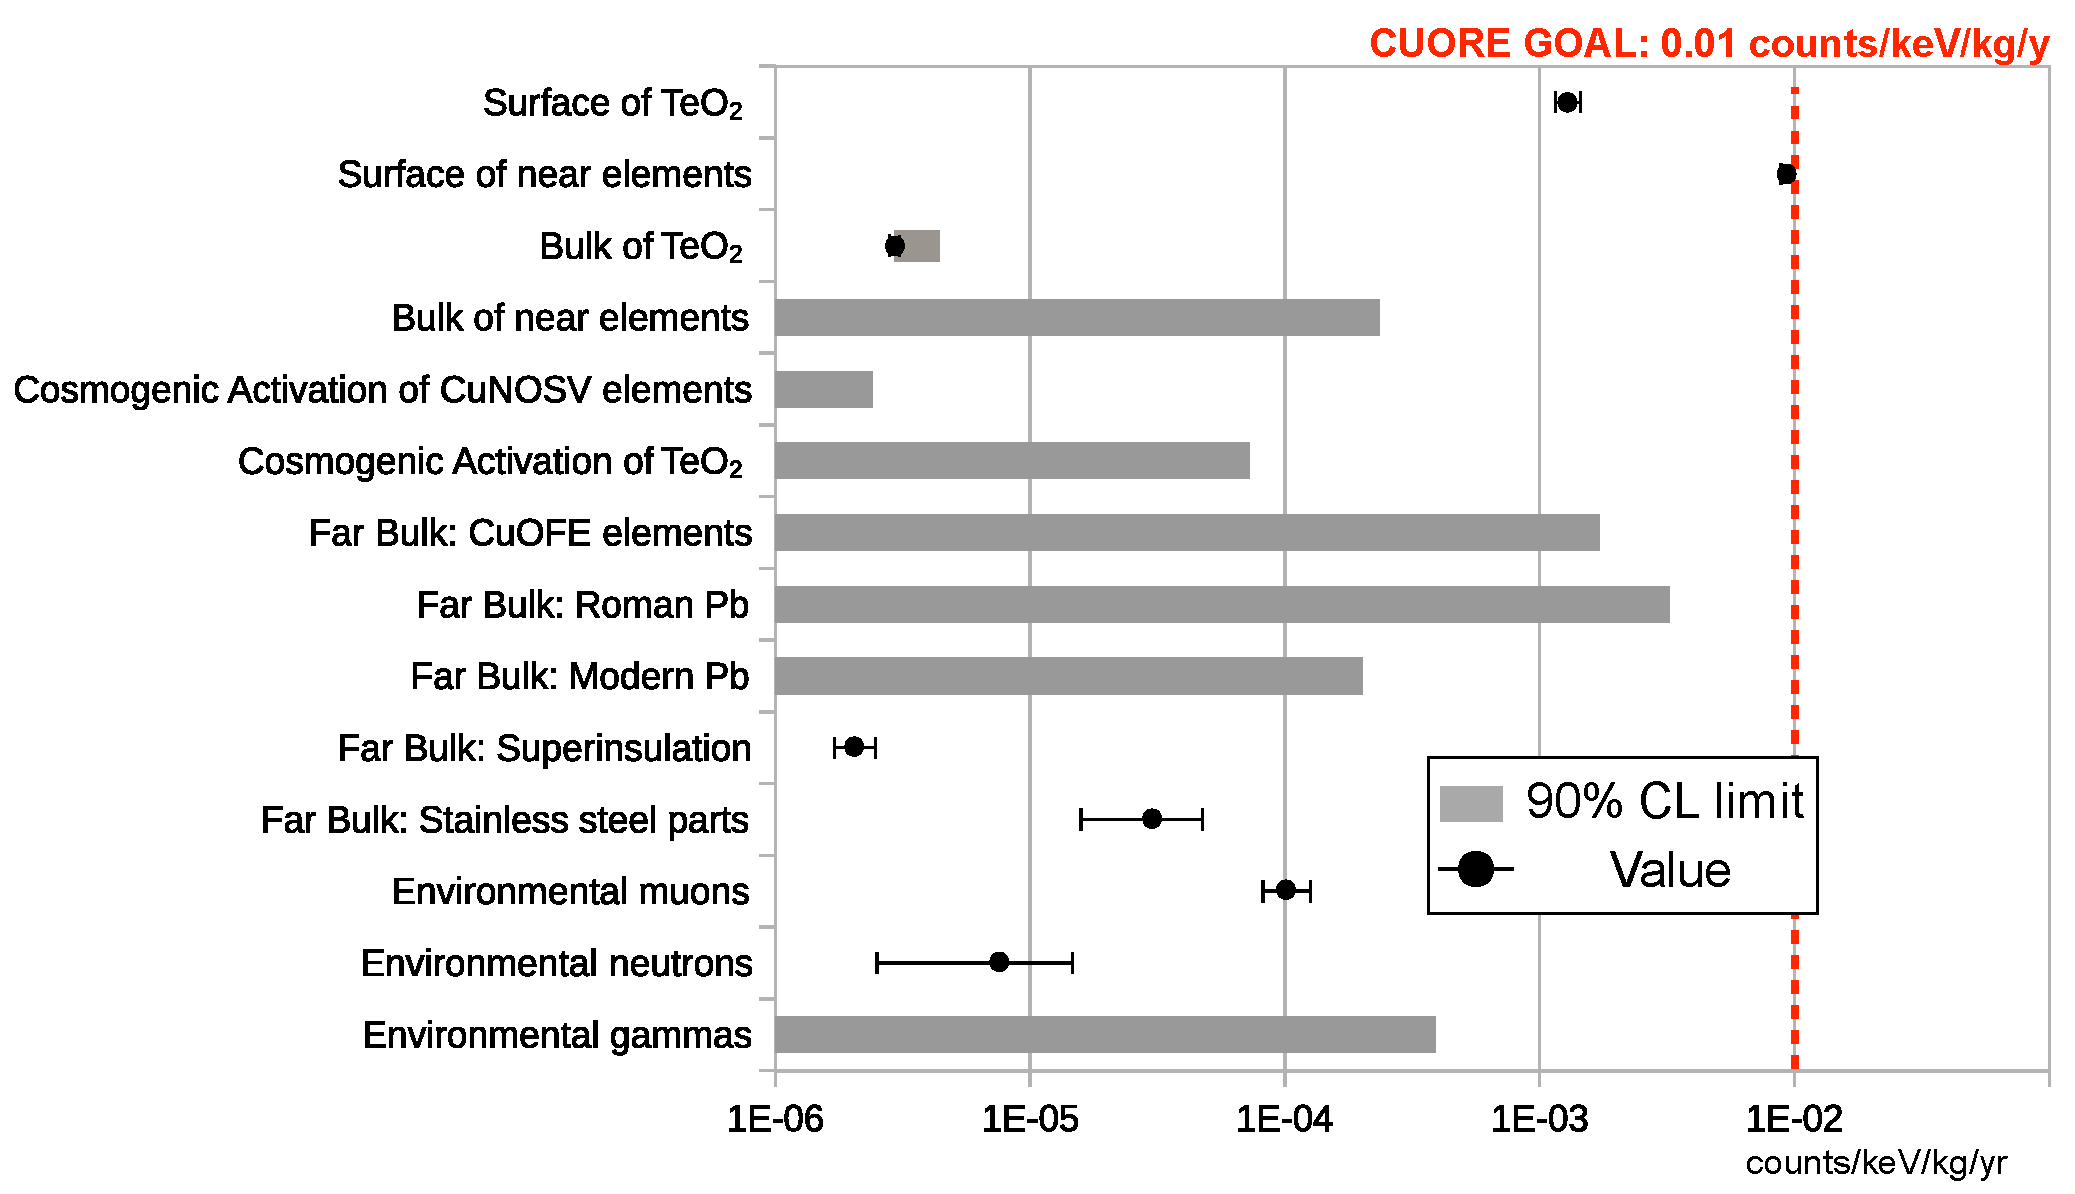
\includegraphics[width=0.8\linewidth]{Figures/CUORE_background_budget}
\caption[CUORE background budget.]
{CUORE background budget.
The CUORE goal is 0.01 counts/keV/kg/y with most of the background due to the surfaces of cryostat elements nearest to the crystal and the bulk of the Roman lead.}
\label{fig:cuore_background_budget}
\end{figure}